\documentclass[11pt,twoside]{article}
\usepackage{fancyhdr}
\usepackage[colorlinks,citecolor=blue,urlcolor=blue,linkcolor=blue,bookmarks=false]{hyperref}
\usepackage{amsfonts,epsfig,graphicx}
\usepackage{afterpage}
\usepackage{amsmath,amssymb,amsthm} 
\usepackage{fullpage}
\usepackage{epsf} 
\usepackage{graphics} 
\usepackage{amsfonts,amsmath}
\usepackage[sort,numbers]{natbib} 
\usepackage{psfrag,xspace}
\usepackage{color,etoolbox}

\setlength{\textwidth}{\paperwidth}
\addtolength{\textwidth}{-6cm}
\setlength{\textheight}{\paperheight}
\addtolength{\textheight}{-4cm}
\addtolength{\textheight}{-1.1\headheight}
\addtolength{\textheight}{-\headsep}
\addtolength{\textheight}{-\footskip}
\setlength{\oddsidemargin}{0.5cm}
\setlength{\evensidemargin}{0.5cm}
\renewcommand{\floatpagefraction}{.8}%

\newtheorem{theorem}{Theorem} 
\newtheorem{lemma}{Lemma}
\newtheorem{proposition}{Proposition}
\newtheorem{corollary}{Corollary}
\newtheorem{definition}{Definition}
\newtheorem*{remark}{Remark}

\usepackage[utf8]{inputenc} % allow utf-8 input
\usepackage[T1]{fontenc}    % use 8-bit T1 fonts
\usepackage{hyperref}       % hyperlinks
\usepackage{url}            % simple URL typesetting
\usepackage{booktabs}       % professional-quality tables
\usepackage{amsfonts}       % blackboard math symbols
\usepackage{nicefrac}       % compact symbols for 1/2, etc.
\usepackage{microtype}      % microtypography

\usepackage{microtype}
\usepackage{graphicx}
\usepackage{float}
\usepackage[export]{adjustbox}
\usepackage{subcaption}
\usepackage{booktabs}
\usepackage{xcolor}
%\usepackage{xr-hyper}
%\usepackage{hyperref}
%\usepackage[reqno]{amsmath}
%\usepackage{amsfonts, amsthm, amssymb}
\usepackage{algorithm}
\usepackage{algorithmic}
%\usepackage[parfill]{parskip}
\usepackage{enumerate}
\usepackage[shortlabels]{enumitem}
\usepackage{bm}
\usepackage{mathtools}

%%%%%% Begin Alden


\newcommand{\diam}{\rho}
\newcommand{\set}[1]{\left\{#1\right\}}
\newcommand{\seq}[1]{\left\{#1\right\}_{n \in \mathbb{N}}}
\newcommand{\defeq}{\overset{\mathrm{def}}{=}}
\newcommand{\vol}{\mathrm{vol}}
\newcommand{\cut}{\mathrm{cut}}
\newcommand{\abs}[1]{\left \lvert #1 \right \rvert}
\newcommand{\N}{\mathbb{N}}
\newcommand{\Reals}{\mathbb{R}}
\newcommand{\Rd}{\Reals^d}
\newcommand{\norm}[1]{\left\lVert#1\right\rVert}
\newcommand{\1}{\mathbf{1}}
\newcommand{\Phibf}{\Phi_{u}}
\newcommand{\Psibf}{\Psi_{u}}
\newcommand{\taubf}{\tau_{u}}
\newcommand{\dist}{\mathrm{dist}}
\newcommand{\Err}{\mathrm{Err}}
\newcommand{\TV}{\mathrm{TV}}

%%% Vectors
\newcommand{\pbf}{p}        % removed bold font
\newcommand{\qbf}{\mathbf{q}}
\newcommand{\ebf}[1]{{e}_{#1}}
\newcommand{\pibf}{\pi}

%%% Matrices (no bold font)
\newcommand{\Abf}{A}
\newcommand{\Xbf}{X}             % removed bold font 
\newcommand{\Wbf}{W}
\newcommand{\Lbf}{L}
\newcommand{\Dbf}{D}
\newcommand{\Ibf}[1]{I_{#1}}

%%% Probability distributions (and related items)
\newcommand{\Pbb}{\mathbb{P}}
\newcommand{\Cbb}{\mathbb{C}}
\newcommand{\Ebb}{\mathbb{E}}

%%% Sets
\newcommand{\Sset}{\mathcal{S}}
\newcommand{\Cset}{\mathcal{C}}
\newcommand{\Aset}{\mathcal{A}}
\newcommand{\Asig}{\Aset_{\sigma}}
\newcommand{\Csig}{\Cset_{\sigma}}
\newcommand{\Asigr}{\Aset_{\sigma,\sigma + r}}
\newcommand{\Csigr}{\Cset_{\sigma,\sigma + r}}

%%% Graph quantities
\newcommand{\Cest}{\widehat{C}}
\newcommand{\degminpr}{d_{\min}'}
\newcommand{\degminwt}{\widetilde{d}_{\min}}
\newcommand{\degmaxwt}{\widetilde{d}_{\max}}
\newcommand{\degmax}{d_{\max}}
\newcommand{\piminwt}{\widetilde{\pi}_{\min}}
\newcommand{\piminpr}{\pibf_{\min}'}
\newcommand{\degmin}{d_{\min}}

%%% Operators
\DeclareMathOperator*{\argmin}{arg\,min}
\newcommand{\dx}{\,dx}
\newcommand{\dy}{\,dy}
\newcommand{\dt}{\,dt}

%%% Algorithm notation
\newcommand{\ppr}{{\sc PPR}}
\newcommand{\pprspace}{{\sc PPR~}}

%%% Tilde notation for quantities over the expansion set 
\newcommand{\wn}{\widetilde{n}}
\newcommand{\wX}{\widetilde{\Xbf}}
\newcommand{\wx}{\widetilde{x}}
\newcommand{\wz}{\widetilde{z}}
\newcommand{\wbz}{\widetilde{\bf{z}}}
\newcommand{\wu}{\widetilde{u}}
\newcommand{\wPbb}{\widetilde{\Pbb}}
\newcommand{\wf}{\widetilde{f}}
\newcommand{\wDbf}{\widetilde{\Dbf}}
\newcommand{\piwt}{\widetilde{\pi}}

\newcommand{\sbcomment}[1]{{\color{red} \bf{{{{SB --- #1}}}}}}

%\newtheoremstyle{aldenthm}
%{6pt} % Space above
%{6pt} % Space below
%{\itshape} % Body font
%{} % Indent amount
%{\bfseries} % Theorem head font
%{.} % Punctuation after theorem head
%{.5em} % Space after theorem head
%{} % Theorem head spec (can be left empty, meaning `normal')

%\theoremstyle{aldenthm}
%\newtheorem{theorem}{Theorem}
%\newtheorem{definition}{Definition}
%\newtheorem{lemma}{Lemma}
%\newtheorem{proposition}{Proposition}
%\newtheorem{corollary}{Corollary}

%\newtheoremstyle{aldenrmrk}
%{6pt} % Space above
%{6pt} % Space below
%{} % Body font
%{} % Indent amount
%{\itshape} % Theorem head font
%{.} % Punctuation after theorem head
%{.5em} % Space after theorem head
%{} % Theorem head spec (can be left empty, meaning `normal')
%
%\theoremstyle{aldenrmrk}
%\newtheorem{remark}{Remark}
%%%%%% End Alden

%\title{Local Spectral Clustering of Density Upper Level Sets}

% The \author macro works with any number of authors. There are two commands
% used to separate the names and addresses of multiple authors: \And and \AND.
%
% Using \And between authors leaves it to LaTeX to determine where to break the
% lines. Using \AND forces a line break at that point. So, if LaTeX puts 3 of 4
% authors names on the first line, and the last on the second line, try using
% \AND instead of \And before the third author name.
%
%\author{
%Alden Green \And
%Sivaraman Balakrishnan \And
%Ryan J. Tibshirani}
%
%\begin{document}
%\maketitle
%
%\vspace{0.1in}
%\begin{abstract}


\newcommand{\widgraph}[2]{\includegraphics[keepaspectratio,width=#1]{#2}}
\newcommand{\Like}{\ensuremath{\mathcal{L}}}
\newcommand{\Ball}[2]{\mathbb{B}_{#1}(#2)}
\newcommand{\Complement}[1]{\overline{#1}}

\newcommand{\xsam}{\ensuremath{x}}
\newcommand{\samind}{\ensuremath{\ell}}
\newcommand{\Xrv}{\ensuremath{X}}
\newcommand{\Event}{\ensuremath{\mathcal{E}}}
\newcommand{\Fevent}{\ensuremath{\mathcal{F}}}

\newcommand{\usedim}{\ensuremath{d}}
\newcommand{\mubold}{\ensuremath{\boldsymbol{\mu}}}
\newcommand{\lambold}{\ensuremath{\boldsymbol{\lambda}}}
\newcommand{\sep}{\ensuremath{\xi}}
\newcommand{\mixind}{\ensuremath{i}}
\newcommand{\mixtwo}{\ensuremath{j}}
\newcommand{\nummix}{\ensuremath{M}}
\newcommand{\mustar}{\ensuremath{\mu^*}}
\newcommand{\muboldstar}{\ensuremath{\mubold^*}}
\newcommand{\muboldt}{\ensuremath{\mubold^t}}

\newcommand{\numobs}{\ensuremath{n}}
\newcommand{\SamLike}{\ensuremath{\Like_\numobs}}
\newcommand{\PopLike}{\ensuremath{\Like}}
\newcommand{\Exs}{\E}
\newcommand{\thetanew}{\ensuremath{\theta^{\text{\small{new}} }}}

\newcommand{\stepsize}{\ensuremath{s}}


\newcommand{\QMAT}{\ensuremath{\mathbf{Q}}} 
\newcommand{\DMAT}{\ensuremath{\mathbf{D}}} 

\newcommand{\defn}{\ensuremath{: \, =}}
\newcommand{\muboldtilde}{\ensuremath{\tilde{\mubold}}}

%%% New version of \caption puts things in smaller type, single-spaced 
%%% and indents them to set them off more from the text.
\makeatletter
\long\def\@makecaption#1#2{
        \vskip 0.8ex
        \setbox\@tempboxa\hbox{\small {\bf #1:} #2}
        \parindent 1.5em  %% How can we use the global value of this???
        \dimen0=\hsize
        \advance\dimen0 by -3em
        \ifdim \wd\@tempboxa >\dimen0
                \hbox to \hsize{
                        \parindent 0em
                        \hfil 
                        \parbox{\dimen0}{\def\baselinestretch{0.96}\small
                                {\bf #1.} #2
                                %%\unhbox\@tempboxa
                                } 
                        \hfil}
        \else \hbox to \hsize{\hfil \box\@tempboxa \hfil}
        \fi
        }
\makeatother



%%%%%%%%%%%%%%%%%%%%%%%%%%%%%%%%%%%%%%%%%%%%%%%%%%%%%%%%%%%%%%%%%%%%%%%%%%%%%%

\begin{document}



\begin{center} {\Large{\bf{Local Spectral Clustering of Density Upper Level Sets}}}

\vspace*{.3cm}

{\large{
\begin{center}
Alden Green ~~~~~ Sivaraman Balakrishnan~~~~~ Ryan Tibshirani\\
\vspace{.2cm}
\end{center}


\begin{tabular}{c}
Department of Statistics and Data Science \\
Carnegie Mellon University
\end{tabular}

\vspace*{.2in}

\begin{tabular}{c}
\texttt{\{ajgreen,sbalakri,ryantibs\}@andrew.cmu.edu}
\end{tabular}
}}

\vspace*{.2in}

\today
\vspace*{.2in}

\begin{abstract}
\noindent We analyze the Personalized PageRank (PPR) algorithm, a local spectral method for clustering,
which extracts clusters using locally-biased random walks around a user-specified
seed node.  In contrast to previous work, we adopt a traditional statistical
learning setup, where we obtain samples from an unknown distribution, and aim to
identify connected regions of high-density (density clusters).  We prove that
PPR, run on a neighborhood graph, extracts sufficiently salient density
clusters, and conversely fails to recover geometrically poorly conditioned density clusters. We also provide empirical support to illustrate our theoretical results.
\end{abstract}
\end{center}
\section{Introduction}
\label{sec: introduction}
In this paper, we consider the problem of clustering: splitting a given data set
into groups that satisfy some notion of within-group similarity and
between-group difference.  Our particular focus is on
spectral clustering methods, a family of powerful
nonparametric clustering algorithms. Roughly speaking, a spectral algorithm
first constructs a geometric graph $G$, where vertices correspond to samples,
and edges correspond to proximities between samples. The algorithm 
then estimates a feature
embedding based on (an appropriate) Laplacian matrix of the graph 
$G$, and applies a simple clustering
technique (like $k$-means clustering) in the embedded feature space.

% Spectral clustering and density clustering
%Spectral clustering algorithms, which
%originated in the early work of Fiedler \cite{fiedler73}, have seen a recent revival 
%(see for instance the recent review~\cite{XX}) focused mainly on understanding the performance of spectral clustering on the Stochastic Block Model (SBM) and closely related problems.
%A parallel line of work \cite{shi09,schiebinger15}, has considered spectral partitioning applied to a non-parametric mixture model
%where once again the clustering goal is to recover the latent labels of a sample $X_1,\ldots,X_n \sim P$. These works proceed by relating the eigenvectors of the graph Laplacian to eigenfunctions of an appropriately defined integral operator, and then using assumptions about the (non-)overlap of the mixture components to show that these eigenfunctions elucidate the latent labels. 

When applied to geometric graphs built from a large number of samples,
global spectral clustering methods can be computationally cumbersome and   
insensitive to the local geometry of the underlying distribution
\citep{leskovec2010,mahoney2012}.  This has led to increased interest in
local spectral clustering algorithms, which leverage locally-biased spectra
computed using random walks around some user-specified seed node.  A popular 
local clustering algorithm is the Personalized PageRank (PPR) algorithm, first introduced by 
\citet{haveliwala2003}, then further developed by
several others~\citep{spielman2011,spielman2014,andersen2006,mahoney2012,zhu2013}.

Local spectral clustering techniques have been practically very successful
\citep{leskovec2010,andersen2012,gleich2012,mahoney2012,wu2012}, leading 
many authors to develop supporting theory
\citep{spielman2013,andersen2009,gharan2012,zhu2013} that gives worst-case
guarantees on traditional graph-theoretic notions of cluster quality (such as
conductance).  In this paper, we adopt a classical statistical viewpoint,
and examine what the output of local clustering on a data set reveals about the
underlying density of the samples 
$f$.  In particular, we examine the ability of PPR to recover
\emph{density clusters} of $f$, defined as the connected components of
the upper level set $\{x \in \Rd : f(x) \geq \lambda\}$ for some $\lambda > 0$
(a central object of interest in the statistical clustering literature, dating
back to the work of \citet{hartigan1981}).   

\section{Background and Related Work}
We begin by providing some standard background on the PPR algorithm
and the density clustering setup, before turning our attention to related work
and a
detailed summary of our contributions.

\subsection{PPR on a neighborhood graph} 
We now describe the clustering
algorithm that will be our focus for the rest of the paper. Let $\Xbf = \{x_1,
\ldots, x_n\}$ be a sample drawn i.i.d.\ from a distribution $\Pbb$ on $\Rd$,
with density~$f$.  For a radius $r > 0$, we define $G_{n,r}=(V,E)$ to be the
\emph{$r$-neighborhood graph} of $\Xbf$, an unweighted, undirected graph with
vertices $V=\Xbf$, and an edge $(x_i,x_j) \in E$ if and only if $\norm{x_i -
x_j} \leq r$, where $\norm{\cdot}$ is the Euclidean norm. We denote by $\Abf \in
\Reals^{n \times n}$ the adjacency matrix, with entries $\Abf_{uv} = 1$ if
$(u,v) \in E$ and $0$ otherwise.  We also denote by $\Dbf$ the diagonal degree
matrix, with entries $\Dbf_{uu} := \sum_{v \in V} \Abf_{uv}$, and by $\Ibf{}$ the $n
\times n$ identity matrix.

Next, we define the PPR vector $\pbf_v = \pbf(v,\alpha;G_{n,r})$, based on
a seed node $v \in V$ and a teleportation parameter $\alpha \in [0,1]$, to be 
the solution of the following linear system:
\begin{equation}
\label{eqn: ppr_vector}
\pbf_v = \alpha \ebf{v} + (1 - \alpha) \pbf \Wbf,
\end{equation}
where $\Wbf = (\Ibf{} + \Dbf^{-1}\Abf)/2$ is the lazy random walk matrix over
$G_{n,r}$ and $e_{v}$ is the indicator vector for node $v$ (that has a 1 in the
$v$-th position and 0 elsewhere). 

\subsection{Sweep cut.}
\label{subsection: sweep_cut}

We employ the sweep cut method to obtain a local cluster from the PPR embedding $\pbf_v$. For a level $\beta > 0$, we define a \emph{$\beta$-sweep cut} of $\pbf_v = (\pbf_v(u))_{u \in V}$
as   
\begin{equation}
\label{eqn: sweep_cuts}
S_{\beta,v} := \set{u \in V: \frac{\pbf_v(u)}{\Dbf_{uu}} > \beta}.
\end{equation}
We will use the normalized cut metric to determine which sweep cut $S_{\beta}$
is the best cluster estimate. For a set $S \subseteq V$ with complement $S^c = V
\setminus S$, we define \smash{$\cut(S;G_{n,r}) := \sum_{u \in S, v \in S^c}
\Abf_{uv}$}, and \smash{$\vol(S; G_{n,r}) := \sum_{u \in S} \Dbf_{uu}$}.  We
define the \emph{normalized cut} of $S$ as
\begin{equation}
\label{eqn: normalized_cut}
\Phi(S; G_{n,r}) := \frac{\cut(S;G_{n,r})}{\min \set{\vol(S; G_{n,r}), \vol(S^c; G_{n,r})}}.
\end{equation}
Having computed sweep cuts $S_{\beta}$ over a range \smash{$\beta \in  
(L, U)$} (where the range $(L,U)$ is also a user-specified parameter), we output the cluster estimate
\smash{$\Cest = S_{\beta^*}$} that has minimum normalized cut.
%\smash{$\Phi(S_{\beta^*}; G_{n,r})$}. 
For concreteness, the PPR algorithm is summarized in Algorithm~\ref{alg: ppr}. 

\begin{algorithm}
\caption{PPR on a neighborhood graph}
\label{alg: ppr}	
{\bfseries Input:} data $\Xbf=\{x_1,\ldots,x_n\}$, radius $r > 0$, teleportation
parameter $\alpha \in [0,1]$, seed $v \in \Xbf$, sweep cut range $(L,U)$. \\     
{\bfseries Output:} cluster $\Cest \subseteq V$.
\begin{algorithmic}[1]
  \STATE Form the neighborhood graph $G_{n,r}$.
  \STATE Compute the PPR vector $\pbf_v=\pbf(v, \alpha; G_{n,r})$ as in \eqref{eqn: 
    ppr_vector}. 
  \STATE For \smash{$\beta \in (L,U)$} compute sweep cuts 
  $S_{\beta}$ as in \eqref{eqn: sweep_cuts}.
  \STATE Return the cluster \smash{$\Cest = S_{\beta^*}$}, where  
  $$
  \beta^* = \argmin_{\beta \in (L,U)}~ \Phi(S_{\beta}; G_{n,r}).
  $$
\end{algorithmic}
\end{algorithm}

\subsection{Estimation of density clusters} 
Let \smash{$\Cbb_f(\lambda)$} denote 
the connected components of the density upper level set $\{x \in \Rd: f(x) >
\lambda\}$.  For a given density cluster \smash{$\Cset \in \Cbb_f(\lambda)$}, we
call $\Cset[\Xbf] = \Cset \cap \Xbf$ the \emph{empirical density cluster}. The size of the symmetric set difference between estimated and empirical cluster is 
a commonly used metric to quantify cluster estimation error
\citep{korostelev1993,polonik1995,rigollet2009}. We will consider a related metric, the volume of the symmetric set difference, which weights points according to their degree in $G_{n,r}$. 
\begin{definition}
	\label{def:volume_symmetric_set_difference}
	For an estimator $\widehat{C} \subseteq \Xbf$ and a set $\mathcal{S} \subseteq \Rd$, the symmetric set difference is 
	\begin{equation*}
	\widehat{C} \vartriangle \mathcal{S}[\Xbf] := \bigl(\widehat{C} \cap \setminus \mathcal{S}[\Xbf]\bigr) \cup \bigl(\Xbf\setminus\widehat{C} \cap \mathcal{S}[\Xbf]\bigr).
	\end{equation*}
	We will measure the discrepancy of $\widehat{C}$ to the set $\mathcal{S}[\Xbf]$ by the volume of the symmetric set difference,
	\begin{equation*}
	\Delta(\widehat{C}, \mathcal{S}[\Xbf]) := \vol(\widehat{C} \vartriangle \mathcal{S}[\Xbf]; G_{n,r})
	\end{equation*}
\end{definition}
However, the symmetric set difference does not measure whether \smash{$\Cest$} 
can distinguish any two distinct clusters \smash{$\Cset,\Cset' \in
\Cbb_f(\lambda)$}. We therefore also study a second notion of cluster
estimation, first introduced by \citet{hartigan1981}, and defined
asymptotically. 

\begin{definition}[Consistent density cluster estimation]
  \label{def: consistent_density_cluster_estimation}
  For an estimator \smash{$\Cest \subseteq \Xbf$} and cluster 
  \smash{$\Cset \in \Cbb_f(\lambda)$}, we say \smash{$\Cest$} is a consistent 
  estimator of $\Cset$ if for all \smash{$\Cset' \in \Cbb_f(\lambda)$} with
  $\Cset \not= \Cset'$, the following holds as $n \to \infty$: 
  \begin{equation}
    \label{eqn: consistent_density_cluster_recovery}
    \Cset[\Xbf] \subseteq \Cest \quad \text{and} \quad
    \Cest \cap \Cset'[\Xbf] = \emptyset,
  \end{equation}
  with probability tending to 1.
\end{definition}
\noindent Consistent cluster recovery roughly ensures that, for a given density threshold $\lambda$, the estimated cluster $\Cest$ contains all
points in a true
density cluster $\Cset \in \Cbb_f(\lambda)$, and simultaneously does not contain any points in any other density cluster $\Cset' \in \Cbb_f(\lambda)$. 

With these definitions in place, our broad goal will be to understand the extent to which the PPR algorithm is able to
recover a cluster which either guarantees low symmetric set difference to a true density cluster, or which consistently estimates
a true density cluster.

%\subsection{Our Contributions} 


\subsection{Related Work and Our Contributions}
In addition to the background on local spectral
clustering given previously, a few related lines of work are worth
highlighting. In the stochastic block model (SBM), arguably one of the simplest models of network formation, edges between nodes independently occur with probability based on a latent community membership. The ability of spectral algorithms to perform clustering -- community detection-- in this context is well-understood. In particular, \citet{rohe2011} upper bound the fraction of nodes misclassified by a spectral algorithm for the high-dimensional (large number of blocks) SBM,  \citet{lei2015} extend these results to the sparse (low average degree) regime, and \citet{balakrishnan2011} analyze the misclassification rate when the block model exhibits some hierarchical structure. The framework we consider, where nodes correspond to data points sampled from an underlying density, and edges between nodes are formed based on geometric proximity, is quite different than the SBM, and therefore so is our analysis.

The study of spectral algorithms on neighborhood graphs has focused on establishing consistency results-- that is, asymptotic convergence of eigenvalues and eigenvectors of matrices to eigenvalues and eigenfunctions of limiting operators. \citet{koltchinskii2000} establish convergence of spectral projections of the adjacency matrix to a limiting integral operator, with similar results obtained using simplified proofs in \citet{rosasco10}. \citet{vonluxburg2008} studies convergence of eigenvectors of the Laplacian matrix for a neighborhood of fixed radius. \citet{belkin07} and \citet{garciatrillos18} extend these results to the regime where the radius $r \to 0$ as $n \to \infty$.


These results are of fundamental importance; however, the behavior of the spectra of these continuum operators can in general be hard to grasp. Therefore, further work relating this spectra to the geometry of the distribution $\Pbb$ is of interest. In this spirit, \citet{shi2009,schiebinger2015,garciatrillos19} examine the ability of  
spectral algorithms to recover the latent labels in certain geometrically well-conditioned nonparametric mixture models. Their results focus on global rather than local 
methods, and thus impose global rather than local conditions on the nature
of the density. Moreover, they do not in general guarantee recovery of density 
clusters, which is the focus in our work. Perhaps most importantly, these works
rely on general cluster saliency conditions, which implicitly depend on many
distinct geometric aspects of the cluster $\Cset$ under consideration. We make
this dependence more explicit, and in doing so expose the role each geometric
condition plays in the clustering problem. 

A substantial portion of our technical effort involves estimating graph-theoretic connectivity properties of empirical density clusters in the neighborhood graph $G_{n,r}$. In particular, we prove an upper bound on the mixing time of a random walk run only over the subset of nodes in $G_{n,r}$ which fall within a density cluster $\Cset$. To do so, we rely on a series of seminal works upper bounding the mixing time of \emph{geometric random walks} (see \citet{vempala2005} for a comprehensive review.)  This study was initiated by \citet{dyer1991}, who used geometric random walks as a fundamental subroutine to efficiently compute volumes of high-dimensional convex bodies. These results are improved in \citet{lovasz1990,kannan97,kannan06}, who show \textit{inter alia} that the bounds on mixing time can be sharpened by avoiding so-called ``start-penalties''.(These improvements are crucial to our work, for they allow us to avoid factors of $\log n$ which would imply divergence as $n \to \infty$.) Following the lead of \citet{abbasi-yadkori2016,abbasi-yadkori2016a}, we extend these results to hold for Lipschitz deformations of convex sets. Additionally, we relate the mixing time of these (continuous-space) geometric random walks to the mixing time of random walks over (discrete) neighborhood graphs.

Finally, it is worth mentioning that density clustering and level set estimation are well-studied problems. \citet{polonik1995, rigollet2009} study density clustering under the 
symmetric set difference metric, \citet{tsybakov1997, singh2009} describe
minimax optimal level-set estimators under Hausdorff loss and
\citet{hartigan1981, chaudhuri2010, balakrishnan2013} consider consistent estimation of the
cluster tree.
%, to note but a few works. 
We emphasize that our goal is not to improve on these
results, nor to offer a better algorithm for level set estimation; indeed, seen as
a density clustering algorithm, PPR has none of the optimality guarantees 
found in the aforementioned works. Instead, our motivation is to start with a 
widely-used local spectral method, PPR, and to better understand and
characterize the distinctions between those density clusters which are
well-conditioned for PPR, and those which are not. 


Specifically, a summary of our results (and an outline for this
paper) is as follows.

\begin{enumerate}
\item In Section \ref{sec: consistent_cluster_estimation_with_ppr}, we introduce
  a set of natural geometric conditions on the density cluster $\Cset$
  %formalize a measure of difficulty based on these geometric conditions, 
  and show that when Algorithm \ref{alg: ppr} is properly initialized, the size of
  the symmetric set difference of \smash{$\Cest$} and a thickened version of the
  density cluster $\Csig$ can be bounded in a meaningful way.
  % this difficulty measure.  
	
\item We further show in Section \ref{sec:
    consistent_cluster_estimation_with_ppr} that if the density cluster 
  $\Cset$ is particularly well-conditioned, Algorithm \ref{alg: ppr}
  will consistently estimate a density cluster in the sense of
  \eqref{eqn: consistent_density_cluster_recovery}. 
	
\item In Section \ref{sec: analysis}, we detail some of the analysis required to
  prove our main results, and expose the parts various geometric quantities play 
  in the difficulty of the clustering problem. 
  
\item In Section \ref{sec:lower_bound}, we provide an accompanying lower bound, demonstrating that when the cluster $\Cset$ is sufficiently poorly conditioned, it will not be recovered by Algorithm~\ref{alg: ppr}.
	
\item In Section \ref{sec: experiments}, we empirically investigate the
  tightness of our analysis, and provide examples showing how violations of our
  geometric conditions impact density cluster recovery by PPR.
\end{enumerate}

\noindent At this point we summarize one of our main takeaways: 
PPR, run on a neighborhood graph, recovers only \emph{geometrically
compact} high-density clusters. Our main theoretical results, make this takeaway 
precise, and provide concrete ways of quantifying the geometric
compactness of a density cluster. 

\section{Main Results}
\label{sec: consistent_cluster_estimation_with_ppr}
In this section we present our main results on the accuracy of the PPR algorithm 
for recovering density clusters. 
We begin by formally introducing a variety of geometric conditions, 
and use these to define a condition
number $\kappa(\Cset)$, which measures the difficulty PPR will have in  
estimating a density cluster $\Cset$.
With this condition in place 
our first main result (Theorem~\ref{thm:volume_ssd}) provides a bound
on the symmetric set difference between the estimated cluster $\Cest$,
obtained by an appropriately initialized version of the PPR algorithm,
and
the target cluster $\Cset$.
Our next main result (Theorem~\ref{thm: consistent_recovery_of_density_clusters})
shows that for sufficiently well-conditioned target clusters $\Cset$, the output 
of the PPR algorithm $\Cest$
is consistent in the sense defined in Definition~\ref{def: consistent_density_cluster_estimation}.

\subsection{Preliminaries}%: Geometric Conditions and the Condition Number of a Density Cluster}
%We formalize some geometric conditions, and use these to define a condition
%number $\kappa(\Cset)$, which measures the difficulty PPR will have in  
%estimating $\Cset$. (Our theoretical guarantees for PPR will be framed in terms 
%of $\kappa(\Cset)$.)
%\paragraph{Geometric conditions on density clusters.} 
At a high level, for PPR
to be successful, the underlying density cluster must be geometrically
well-conditioned.  A basic requirement is that we need to avoid clusters which contain arbitrarily
thin bridges or spikes. As in the work of \citet{chaudhuri2010}, we consider a
thickened version of \smash{$\Cset \in \Cbb_f(\lambda)$} defined as 
$\Csig := \set{x \in \Reals^d: \dist(x,\Cset) \leq \sigma}$, which 
we call the \emph{$\sigma$-expansion} of $\Cset$. Here 
\smash{$\dist(x,\Cset) := \inf_{y \in \Cset} \norm{y - x}$}.  We now list our
conditions on $\Csig$.

\begin{enumerate}[label=(A\arabic*)]
\item
  \label{asmp: bounded_density}
  \emph{Bounded density within cluster:} There exist constants
  $0<\lambda_{\sigma}< \Lambda_{\sigma}<\infty$ such that 
  $\lambda_{\sigma} \leq \inf_{x \in \Csig} f(x) \leq \sup_{x \in \Csig} f(x)
  \leq \Lambda_{\sigma}$. 

    
\item 
  \label{asmp: low_noise_density}
  \emph{Low noise density:} There exists $c_0 > 0$ and $\gamma \in [0,1]$ such that for any $x \in \Rd$ with $0 < \dist(x, \Csig) \leq \sigma$,   
  \begin{align*}
  \inf_{x' \in \Csig} f(x') - f(x) \geq  c_0 \dist(x, \Csig)^{\gamma}. 
  \end{align*}
  Roughly, 
  this assumption ensures that the density decays sufficiently quickly as we move away from
  the target cluster $\Csig$, and is a standard assumption in the level-set estimation literature
  (see for instance~\cite{singh2009}).
  
\item
  \label{asmp: embedding}
  \emph{Lipschitz embedding:}
  There exists $g: \Reals^d \to \Reals^d$ with the following properties: 
  \begin{enumerate}
  \item we have $\Csig = g(\mathcal{K})$, for a convex set $\mathcal{K} \subseteq \Rd$
  with $\mathrm{diam}(\mathcal{K}) = \sup_{x,y \in \mathcal{K}}\norm{x - y} =:
  \diam < \infty$
  \item $\det(\nabla g (x)) = 1$ for all $x \in \Csig$, where
  $\nabla g(x)$ is the Jacobian of $g$ evaluated at $x$ and
  \item for some $L
  \geq 1$,   
  \begin{equation*}
    \norm{g(x) - g(y)} \leq L \norm{x - y} ~
    \text{for all $x,y \in \mathcal{K}$}. 
  \end{equation*}
  \end{enumerate}
  Succinctly, we assume that $\Csig$ is the image of a convex set with finite diameter 
  under a  measure preserving, Lipschitz transformation. 

\item
  \label{asmp: bounded_volume}
  \emph{Bounded volume:}
  For a set $\mathcal{S} \subseteq \Reals^d$, define the $\Pbb$-weighted volume of $\mathcal{S}$ to be
  \begin{equation}
  \label{eqn:volume}
  \vol_{\Pbb,r}(\mathcal{S}) := \int_{\mathcal{S}} \Pbb(B(x,r)) \,d\Pbb(x).
  \end{equation}
  where $B(x,r)$ is the closed ball of radius $r$ centered at $x$.
  
  We assume that neighborhood graph radius $0 < r \leq \sigma/2d$ is chosen such that
  \begin{equation*}
  \vol_{\Pbb,r}(\mathcal{S}) \leq \frac{1}{2}\vol_{\Pbb,r}(\Reals^d).
  \end{equation*}
 
\end{enumerate}

To motivate these conditions, we provide a brief high-level sketch
of our analysis (we return to this more formally in Section~\ref{sec: analysis}). 
\citet{zhu2013} show for an arbitrary graph $G =
(V,E)$ and subset of vertices $S \subseteq V$, the PPR estimate \smash{$\Cest$}
of subset $S$ satisfies, for a constant $c>0$,
\begin{equation}
\label{eqn: graph_symmetric_set_difference_1}
\vol(\Cest \vartriangle S; G) \leq c \bigl( \Phi(S,G)
\cdot \tau_{\infty}(G[S])\bigr),
\end{equation}
where $\Phi(S;G)$ is the normalized cut of $S$ (as defined in \eqref{eqn:
  normalized_cut}), and \smash{$\tau_{\infty}(G[S])$} is  the \emph{mixing
  time} of a random walk over the induced subgraph $G[S]$ (to be defined
precisely later, in \eqref{eqn: mixing_time}).  The left-hand side in
\eqref{eqn: graph_symmetric_set_difference_1} is precisely
the volume of the symmetric set difference, and our main goal is therefore to upper bound the graph functionals $\Phi$ and $\tau_{\infty}$.
  Towards this goal, as we will show in Section \ref{sec:
  analysis}, the conditions \ref{asmp: bounded_density}--\ref{asmp:
  bounded_volume} allow us to upper bound the normalized cut 
\smash{$\Phi(\Csig[\Xbf]; G_{n,r})$}, and the mixing time 
\smash{$\tau_{\infty}(G_{n,r}[\Csig[\Xbf]])$}. In more detail, assumption 
\ref{asmp: low_noise_density} yields an upper
bound on \smash{$\cut(\Csig[\Xbf]; G_{n,r})$}, and \ref{asmp: bounded_density}
yields a lower bound on \smash{$\vol(\Csig[\Xbf]; G_{n,r})$}; together with 
\ref{asmp: bounded_volume}, this gives an upper bound on the normalized cut.  On 
the other hand, \ref{asmp: bounded_density} and \ref{asmp: embedding} preclude
bottlenecks in the induced subgraph \smash{$G_{n,r}[\Csig[\Xbf]]$}, and combined
with the upper bound on diameter in \ref{asmp: embedding}, this leads to an upper bound on
the mixing time over this subgraph.

\subsubsection{Condition number} 
Motivated by \eqref{eqn:
  graph_symmetric_set_difference_1}, we will define $\kappa(\Cset)$ to be an
upper bound on the product \smash{$\Phi(\Csig[\Xbf]; G_{n,r}) \cdot
  \tau_{\infty}(G_{n,r}[\Csig[\Xbf]])$}. Following, the analysis of \citet{zhu2013}
  we see that the smaller $\kappa(\Cset)$ is, the
more success PPR will have in recovering the target cluster $\Cset$.

\begin{definition}[Well-conditioned density clusters]
  \label{def:well_conditioned_density_cluster}
  For $\lambda > 0$ and \smash{$\Cset \in \Cbb_f(\lambda)$}, let $\Cset$ satisfy 
  \ref{asmp: bounded_density}--\ref{asmp: bounded_volume} for some $\sigma > 0$. Then, for universal constants $c_1, c_2, c_3 > 0$ to be specified
  later, we set 
  \begin{equation}
    \label{eqn: condition_number_1}
    \Phibf(\Cset) 
    := c_1 r \frac{d}{\sigma} \frac{\lambda}{\lambda_{\sigma}}
    \frac{(\lambda_{\sigma} - c_0 \frac{r^{\gamma}}{\gamma +
        1})}{\lambda_{\sigma}},~  
    \taubf(\Cset) := c_2 \frac{\Lambda_{\sigma}^4 d^3 \rho^2
      L^2}{\lambda_{\sigma}^4 r^2} \log^2\left(\frac{\Lambda_{\sigma}}{\lambda_{\sigma}^2r}\right) + c_3,
  \end{equation}
  and letting \smash{$\kappa(\Cset) := \Phi_{u}(\Cset) \cdot
    \tau_{u}(\Cset)$}, we call $\Cset$ a 
  \emph{$\kappa$-well-conditioned density cluster}.  
\end{definition}
\noindent The condition number 
$\kappa(\Cset)$ succinctly captures the role of the various
geometric parameters. 
We note in passing that $\Phibf(\Cset)$ and $\taubf(\Cset)$ are exactly the upper bounds 
on \smash{$\Phi(\Csig[\Xbf]; G_{n,r})$} and
\smash{$\tau_{\infty}(G_{n,r}[\Csig[\Xbf]])$} that we derive in our analysis
later, in Section \ref{sec: analysis}. 

\subsubsection{Well-initialized algorithm} As is typical in the local clustering
literature, our algorithmic results will be stated with respect to specific
ranges of each of the user-specified parameters. In particular, for a
well-conditioned density cluster $\Cset$, we require that some of the tuning parameters of Algorithm~\ref{alg: ppr} are chosen to fall within specific ranges,
\begin{equation}
\begin{gathered}
\label{eqn: initialization}
0 < r \leq \frac{\sigma}{2d}, \quad 
\alpha \in [1/10, 1/9) \cdot \frac{1}{\taubf(\theta)}, \\
(L,U) \subseteq (1/50,1/5) \cdot \frac{1}{2{n \choose 2}\vol_{\Pbb,r}(\Csig)}.
\end{gathered}
\end{equation}

\begin{definition}
If the input parameters to Algorithm \ref{alg: ppr} satisfy \eqref{eqn:
  initialization} for some well-conditioned density cluster $\Cset$, we
say the algorithm is \emph{well-initialized}. 
\end{definition}
\noindent In practice it is  not feasible to set hyperparameters based on the
underlying (unknown) density $f$. Typically, one tunes PPR over a range of
hyperparameters and selects the cluster which has the smallest normalized cut. 

\subsection{Cluster Recovery in Symmetric Set Difference}
We now present our first main result: a bound on the volume of the symmetric set difference between the estimated cluster $\widehat{C}$ and empirical cluster $\Csig[\Xbf]$. 
\begin{theorem}
  \label{thm:volume_ssd}
  Fix $\lambda > 0$ and let \smash{$\Cset \in \Cbb_f(\lambda)$} be a
  $\kappa$-well-conditioned density cluster for some $\sigma > 0$. If Algorithm \ref{alg: ppr} is \emph{well-initialized} with respect to $\Cset$, then there exists a universal constant $c > 0$, constants in sample size $c_1(\Pbb,r)$ - $c_6(\Pbb,r)$, and a set $\Csig[\Xbf]^g \subseteq \Csig[\Xbf]$ with $\vol(\Csig[\Xbf]^g; G_{n,r}) \geq \frac{1}{2}\vol(\Csig[\Xbf];G_{n,r})$ such that the following statement holds: let Algorithm~\ref{alg: ppr} be run with any seed node $v \in \Csig[\Xbf]^g$. Then, for any $n$ large enough so that
  \begin{equation*}
  n \geq \max\left\{(\log n)^{\max\{\frac{3}{d},1\}}\left(\frac{1}{c_2(\Pbb,r)}\right)^d, c_3(\Pbb,r)\right\},
  \end{equation*}
  the volume of the symmetric set difference is upper bounded
  \begin{equation}
    \label{eqn:volume_ssd}
    \Delta(\Csig[\Xbf], \Cest) \leq c \cdot \kappa(\Cset) \cdot \vol_{n,r}(\Csig[\Xbf]),
  \end{equation}
  with probability at least $1 - \frac{c_4(\Pbb,r)}{n} - 2n\exp\set{-c_5(\Pbb,r)n} - 2\exp\set{-(c_1(\Pbb,r) + c_6(\Pbb,r))n}$. 
\end{theorem}
The proof of Theorem \ref{thm:volume_ssd} is deferred to Appendix~\ref{sec:proof_of_volume_ssd}. In this theorem, and hereafter, we let $c, c_i > 0$ represent universal constants, and $c_i(\Pbb,r)$ represent constants which depend only on $\Pbb$ and $r$ but not on the sample size $n$; where possible, we keep track of all constants in our proofs. 
This result shows that the volume of the symmetric set difference \smash{$\Delta(\Csig[\Xbf],
  \Cest)$} is upper-bounded by a quantity proportional to the difficulty of the clustering problem, as
measured by the condition number $\kappa(\Cset)$.

\subsection{Consistent Cluster Recovery}
The bound on symmetric set difference \eqref{eqn:volume_ssd} does not imply consistent density cluster estimation in the sense of \eqref{eqn: consistent_density_cluster_recovery}. This notion of consistency requires a uniform bound over $\pbf$: as an example, for all \smash{$\Cset'
  \in \Cbb_f(\lambda), \Cset' \neq \Cset$}, and each $u \in \Cset, w \in
\Cset'$,  
\begin{equation}
\label{eqn: ppr_gap}
\frac{\pbf_v(w)}{D_{ww}} \leq \frac{1}{100 {n \choose 2} \vol_{\Pbb,r}(\Csig)} < \frac{1}{10 {n \choose 2} \vol_{\Pbb,r}(\Csig)} \leq \frac{\pbf_v(u)}{D_{uu}}.
\end{equation}
Then, any $(L,U)$ satisfying~\eqref{eqn: initialization} and any sweep cut $S_{\beta}$ for $\beta \in (L,U)$ will fulfill both conditions
laid out in \eqref{eqn: consistent_density_cluster_recovery}. In Theorem
\ref{thm: consistent_recovery_of_density_clusters}, we show that a sufficiently
small upper bound on $\kappa(\Cset)$ ensures that with high probability the uniform bound~\eqref{eqn: ppr_gap} is satisfied, and hence implies \smash{$\Cest$} will be a consistent  
estimator. We will need one additional regularity condition, to preclude arbitrarily low degree
vertices for points $x \in \Cset'[\Xbf]$. 
\begin{enumerate}[label=(A\arabic*)]
  \setcounter{enumi}{6}
\item 
  \label{asmp: C'_bounded_density}
  \emph{Bounded density in other clusters:} Letting $\sigma,\lambda_{\sigma}$ be 
  as in \ref{asmp: bounded_density}, for each $\Cset' \in \Cbb_f(\lambda)$ and
  for all $x \in \Csig'$, $\lambda_{\sigma} \leq f(x)$. 
\end{enumerate}

Next we give our main result on consistent cluster recovery by PPR.

\begin{theorem}
  \label{thm: consistent_recovery_of_density_clusters}
  Fix $\lambda > 0$, let $\Cset \in \Cbb_f(\lambda)$ be a
  $\kappa$-well-conditioned density cluster for some $\sigma > 0$, and
  additionally assume $f$ satisfies \ref{asmp: C'_bounded_density}. If Algorithm
  \ref{alg: ppr} is well-initialized, there exists a universal constant $c >  0$ and constants in sample size $c_1(\Pbb,r)$-$c_6(\Pbb,r)$ such that if  
  \begin{equation}
    \label{eqn: kappa_ub}
    \kappa(\Cset) \leq c \frac{(\lambda_{\sigma} r^d
      \nu_d)^2}{\vol_{\Pbb,r}(\Csig)}, 
  \end{equation}
  then $\Cest$ satisfies~\eqref{eqn: consistent_density_cluster_recovery} with respect to $\Cset$ with probability at least $1 - \frac{c_4(\Pbb,r)}{n} - 2n\exp\set{-c_5(\Pbb,r)n} - 2\exp\set{-(c_1(\Pbb,r) + c_6(\Pbb,r))n}$. Therefore, $\Cest$ is a consistent estimator of $\Cset$ in the sense of Definition \ref{def: consistent_density_cluster_estimation}. 
\end{theorem}
\noindent Some remarks are in order: 
 \begin{enumerate}  
 \item We note that the restriction on $\kappa(\Cset)$ imposed by \eqref{eqn:
    kappa_ub} results in an upper bound on the symmetric set difference metric \smash{$\Delta(\Csig[\Xbf],
    \Cest)$} on the order of $r^d$. In plain terms, we are able to recover a
  density cluster $\Cset$ in the sense of \eqref{eqn:
    consistent_density_cluster_recovery} only when we can guarantee a very small
  fraction of points will be misclassified. This strong condition is the price
  we pay in order to obtain the uniform bound in~\eqref{eqn: ppr_gap}. 
 \item While taking the radius of the neighborhood graph $r \to 0$ as $n \to
  \infty$ (thereby ensuring that the graph $G_{n,r}$ is sparse) is computationally
  attractive, the presence of a factor of \smash{$\log^2(1/r)/r$} in
  $\kappa(\Cset)$ prevents us from making claims about the
  behavior of PPR in this regime. Although the restriction to a kernel
  function fixed in $n$ is common in spectral clustering theory
  \citep{schiebinger2015,vonluxburg2008}, it is an interesting question whether
  PPR exhibits some degeneracy over $r$-neighborhood graphs as $r \to 0$, or if
  this is merely looseness in our upper bounds.  
\end{enumerate}

\subsection{Approximate PPR vector} 
In practice, exactly solving the system of equations~\eqref{eqn:
  ppr_vector} to compute the PPR vector 
  may be too computationally expensive. To address this limitation,
\citet{andersen2006} introduced the \emph{$\varepsilon$-approximate} PPR vector
(aPPR), which we will denote by \smash{$\pbf^{(\varepsilon)}$}. We refer the
curious reader to \citet{andersen2006} for a formal algorithmic definition of
the aPPR vector, and limit ourselves to highlighting a few salient points: the
aPPR vector can be computed in order $\mathcal{O}(1/(\varepsilon\alpha))$ time,
while satisfying the following uniform error bound: 
\begin{equation}
\label{eqn: appr_error}
\textrm{for all $u \in V$}, \quad \pbf(u) - \varepsilon \Dbf_{uu}\leq
\pbf^{(\varepsilon)}(u) \leq \pbf(u).  
\end{equation}
For a sufficiently small choice of $\varepsilon$, the 
application of \eqref{eqn: appr_error} within the proofs of Theorems \ref{thm:volume_ssd} and \ref{thm: consistent_recovery_of_density_clusters}
leads to analogous results which hold for \smash{$\pbf^{(\varepsilon)}$}. We
formally state and prove this in Corollary~\ref{cor: appr} in 
Appendix~\ref{sec:appr}.

\section{Analysis Overview}
\label{sec: analysis}

One of the primary technical contributions of our work is showing that the geometric
conditions \ref{asmp: bounded_density}--\ref{asmp: bounded_volume} translate to 
meaningful bounds on the normalized cut and mixing time of $\Csig[\Xbf]$ in
$G_{n,r}$. In doing so, we elaborate on how some of the geometric conditions
introduced in Section \ref{sec: consistent_cluster_estimation_with_ppr}
contribute to the difficulty of the clustering problem. 

\subsection{Upper Bound on the Normalized Cut} 
We start with a finite sample upper bound on the
normalized cut \eqref{eqn: normalized_cut} of $\Cset_\sigma[\Xbf]$. For
simplicity, we write $\Phi_{n,r}(\Csig[\Xbf]) := \Phi(\Csig[\Xbf]; G_{n,r})$. 

\begin{theorem}
  \label{thm: conductance_upper_bound}
  Fix $\lambda > 0$, and assume $\Cset \in \Cbb_f(\lambda)$ satisfies
  Assumptions \ref{asmp: bounded_density}--\ref{asmp: low_noise_density}, 
  \ref{asmp: bounded_volume} for some $\sigma > 0$. Then there exists a universal constant $c_1 > 0$ and a constant in sample size $c_1(\Pbb,r)$ such that
  \begin{equation}
    \label{eqn: conductance_additive_error_bound}
    \frac{\Phi_{n,r}(\Csig[\Xbf])}{r} \leq c_1 \frac{d}{\sigma}
    \frac{\lambda}{\lambda_{\sigma}} \frac{(\lambda_{\sigma} -
      c_0\frac{r^{\gamma}}{\gamma+1})}{\lambda_{\sigma}}
  \end{equation}
  with probability at least $1 - 3\exp\{-nc_1(\Pbb,r)\}$. 
\end{theorem}
\noindent {\bf Remark: } 
Observe that the diameter $\rho$ is absent from Theorem \ref{thm:
    conductance_upper_bound}, in contrast to the condition number
  $\kappa(\Cset)$, which worsens (increases) as $\rho$ increases. This
  reflects established wisdom regarding spectral partitioning
  algorithms more generally \citep{guattery1995, hein2010}, albeit newly applied
  to the density clustering setting. It suggests that if the diameter $\rho$ is
  large, PPR may fail to recover $\Csig[\Xbf]$ even when $\Cset$ is
  sufficiently well-conditioned to ensure $\Csig[\Xbf]$ has a small normalized
  cut in $G_{n,r}$. This intuition will be supported by simulations in Section
  \ref{sec: experiments}. 

\subsection{Upper Bounds on the Mixing Time} 
For $S \subseteq V$, denote by $G[S] = (S, E_S)$ the
subgraph induced by $S$ (where the edges are $E_S = E \cap (S \times S)$). Let
$\Wbf_S$ be the (lazy) random walk matrix over $G[S]$, and write  
$$
q_{v}^{(t)}(u) = e_v\Wbf_S^t e_u
$$
for the $t$-step transition probability of the lazy random walk over $G[S]$
originating at $v \in V$. Also write \smash{$\pi = (\pi(u))_{u \in S}$}
for the stationary distribution of this random walk.(As
$\Wbf_S$ is the transition matrix of a lazy random walk, 
it is well-known that a unique stationary distribution exists and is given by 
\smash{$\pi(u) = \deg(u;G[S])/\vol(S; G[S])$}, where we write $\deg(u;G[S]) = \sum_{w \in S} \1((u,w) \in E_S)$ for the degree of $u$ in $G[S]$.) We define the \emph{mixing time} of $G[S]$ as
\begin{equation}
\label{eqn: mixing_time}
\tau_{\infty}(G[S]) = \min\set{ t: \frac{\pi(u) - q_{v}^{(t)}(u)}
  {\pi(u)} \leq \frac{1}{4}, \; \text{for $u,v \in V$}}. 
\end{equation}
Next, we give an asymptotic (in the number of samples $n$) upper bound on
$\tau_{\infty}(G_{n,r}[\Csig[\Xbf]])$.  

\begin{theorem}
  \label{thm: mixing_time_upper_bound}
  Fix $\lambda > 0$, and assume that \smash{$\Cset \in \Cbb_f(\lambda)$}
  satisfies Assumptions \ref{asmp: bounded_density} and \ref{asmp: embedding}
  for some $\sigma > 0$. Additionally assume that the radius $0 < r < \sigma/2\sqrt{d}$. Then there exist universal constants $c_2$ and $c_3$, and constants in sample size $c_2(\Pbb,r)$ - $c_6(\Pbb,r)$ such that the following statement holds: for any
  \begin{equation*}
  n \geq \max\left\{(\log n)^{\max\{\frac{3}{d},1\}}\left(\frac{1}{c_2(\Pbb,r)}\right)^d, c_3(\Pbb,r)\right\}
  \end{equation*}
  the mixing time $\tau_{\infty}(G_{n,r}[\Csig[\Xbf]])$ satisfies
  \begin{equation} 
    \label{eqn: mixing_time_upper_bound}
    \tau_{\infty}(G_{n,r}[\Csig[\Xbf]]) \leq c_2 \frac{\Lambda_{\sigma}^4 d^3 \rho^2 L^2}{\lambda_{\sigma}^4 r^2} \log^2\left(\frac{ \Lambda_{\sigma}}{\lambda_{\sigma}^2 r}\right) + c_3
  \end{equation}
  with probability at least $1 - \frac{c_4(\Pbb,r)}{n} - 2n\exp\set{-c_5(\Pbb,r)n} - 2\exp\set{-c_6(\Pbb,r)n}$.
\end{theorem}

The proof of Theorem \ref{thm: mixing_time_upper_bound} relies heavily on
analogous mixing time bounds developed for the mixing time of a
continuous-space ``ball walk'' over convex sets. To the best of our knowledge, our
result is the first bound on the mixing time of random walks
over neighborhood graphs that is independent of $n$, the number of vertices.   

\vspace{0.2cm}

\noindent {\bf Remark: } 
  The embedding assumption \ref{asmp: embedding} and Lipschitz parameter $L$
  play an important role in proving the upper bound of Theorem \ref{thm:
    mixing_time_upper_bound}. There is some interdependence between $L$ and
  $\sigma,\rho$, which might lead one to hope that \ref{asmp: embedding} is
  non-essential. However, it is not possible to eliminate condition \ref{asmp:
    embedding} without incurring an additional factor of at least
  $(\rho/\sigma)^d$ in \eqref{eqn: mixing_time_upper_bound}, achieved, for
  instance, when $\Csig$ is a dumbbell-like set consisting of two balls of
  diameter $\rho$ linked by a cylinder of radius
  $\sigma$. \citet{abbasi-yadkori2016, abbasi-yadkori2016a}  
  develop theory regarding Lipschitz deformations of convex sets, wherein it
  is observed that star-shaped sets as well as half-moon shapes of the type we
  consider in Section \ref{sec: experiments} both satisfy \ref{asmp: embedding}
  for reasonably small values of $L$. 
  
\section{Lower bound.}
\label{sec:lower_bound}

To show a lower bound for density clustering using PPR, we exhibit a hard case: that is, a distribution $\Pbb$ for which PPR is unlikely to recover a density cluster. Let $\mathcal{C}_{\sigma}^{(0)}$, $\mathcal{C}_{\sigma}^{(1)}$, and $\mathcal{C}_{\sigma}^{(2)}$ be rectangles in $\Reals^2$, 
\begin{equation*}
\mathcal{C}_{\sigma}^{(0)} = \biggl[-\frac{\sigma}{2}, \frac{\sigma}{2}\biggr] \times \biggl[-\frac{\rho}{2}, \frac{\rho}{2}\biggr], \quad \mathcal{C}_{\sigma}^{(1)} = \mathcal{C}_{\sigma}^{(0)} - \set{(\sigma,0)}, \quad \mathcal{C}_{\sigma}^{(2)} = \mathcal{C}_{\sigma}^{(0)} + \set{(\sigma,0)} \tag{$0 < \sigma < \rho$}
\end{equation*}
and let $\mathbb{P}$ be the mixture distribution over $\mathcal{X} = \mathcal{C}_{\sigma}^{(0)} \cup \mathcal{C}_{\sigma}^{(1)} \cup \mathcal{C}_{\sigma}^{(2)}$ given by
\begin{equation*}
\mathbb{P} = \frac{1 - \epsilon}{2} \Psi_1 + \frac{1 - \epsilon}{2} \Psi_2 + \frac{\epsilon}{2} \Psi_0,
\end{equation*}
where $\Psi_m$ is the uniform distribution over $\Csig^{(m)}$ for $m = 0,1,2$. 
The density function $f$ of $\Pbb$ is simply
\begin{equation}
\label{eqn:lb_density}
f(x) = \frac{1}{\rho\sigma}\left(\frac{1 - \epsilon}{2}\1(x \in \mathcal{C}_{\sigma}^{(1)}) + \frac{1 - \epsilon}{2}\1(x \in \mathcal{C}_{\sigma}^{(2)}) + \frac{\epsilon}{2}\1(x \in \mathcal{C}_{\sigma}^{(0)})  \right)
\end{equation}
so that for any $\epsilon < \lambda < (1 - \epsilon)/2$, $\mathbb{C}_{f}(\lambda) = \set{\mathcal{C}_{\sigma}^{(1)}, \mathcal{C}_{\sigma}^{(2)}}$. 

\subsection{Lower bound for PPR.}

As the following theorem demonstrates, even when Algorithm~\ref{alg: ppr} is reasonably initialized, if the density cluster $\mathcal{C}_{\sigma}^{(1)}$ is sufficiently geometrically ill-conditioned the cluster estimator $\widehat{C}$ will fail to recover $\mathcal{C}_{\sigma}^{(1)}$. Let
\begin{equation}
\label{eqn:lower_set}
\mathcal{L} = \set{(x_1,x_2) \in \mathcal{X}: x_2 < 0}.
\end{equation}
\begin{theorem}
	\label{thm:ppr_lb}
	Suppose $r < \frac{1}{40}\rho \wedge \frac{1}{4}\sigma$,  $\alpha = 65 \Phi_{\Pbb}(\mathcal{L})$, and $(L,U) = (0,1)$ are inputs to Algorithm~\ref{alg: ppr}. Then, for any
	\begin{equation}
	\label{eqn:lb_sample_size}
	n \geq \max\set{\frac{64}{\epsilon^2 \rho \sigma \pi r^2}, \frac{8}{\epsilon}}
	\end{equation}
	the following statement holds: there exists a set $C^{g} \subset \Xbf$ with $\vol(C^g \cap \mathcal{C}_{\sigma}^{(1)}[\Xbf]) \geq \frac{1}{10}\vol_{n,r}(\mathcal{C}_{\sigma}^{(1)}[\Xbf])$ such that for any seed node $v \in C^g$, the estimator $\widehat{C}$ computed by Algorithm~\ref{alg: ppr} has symmetric set difference with $\Csig^{(1)}[\Xbf]$ of volume at least
	\begin{equation}
	\label{eqn:ppr_lb}
	\frac{\sigma \rho}{r^2}\frac{\vol_{n,r}(\widehat{C} \vartriangle \mathcal{C}_{\sigma}^{(1)}[\Xbf])}{n^2} \geq \frac{1}{4} -  c \frac{\sqrt{\frac{\sigma}{\rho}}}{\epsilon^2} \sqrt{ \log\left(\frac{\rho \sigma}{\epsilon^2 r^2}\right)\frac{\sigma}{r}}
	\end{equation}
	with probability at least $1 - c_1(\Pbb,r) n \exp\set{-c_2(\Pbb,r)n}$, where $c$ is a universal constant and $c_1(\Pbb,r),c_2(\Pbb,r)$ are constants which do not depend on $n$.
	Consequently, if
	\begin{equation*} 
	\epsilon^2 > \frac{c}{8} \sqrt{\frac{\sigma}{\rho}} \cdot \sqrt{ \log\left(\frac{\rho \sigma}{\epsilon^2 r^2}\right)\frac{\sigma}{r}}
	\end{equation*}
	then with high probability $\frac{\sigma \rho}{r^2}\frac{\vol_{n,r}(\widehat{C} \vartriangle \mathcal{C}_{\sigma}^{(1)}[\Xbf])}{n^2}$ is at least $1/8$. 
\end{theorem}

Note that the factor of $\frac{\sigma\rho}{r^2}$ on the left hand side of \eqref{eqn:ppr_lb} is a constant multiple of $(1/\vol_{\Pbb,r}(\Csig^{(1)}))$; hence the left hand side is directly comparable to $\frac{\vol_{n,r}(\widehat{C} \vartriangle \mathcal{C}_{\sigma}^{(1)}[\Xbf])}{\vol_{n,r}(\Csig^{(1)}[\Xbf])}$, which is the quantity we upper bound in Theorem~\ref{thm:volume_ssd}.

Theorem~\ref{thm:ppr_lb} is stated with respect to a particular hard case, where the density clusters are rectangular subsets of $\Reals^2$. Although we picked this setting to make the theorem statement simple, our results are easily generalized to $\Reals^d$ and to non-rectangular clusters. Additionally, although we state our lower bound with respect to PPR run on neighborhood graph, the conclusion is likely to hold for a much broader class of spectral clustering algorithms. In the proof of Theorem~\ref{thm:ppr_lb}, we rely heavily on the fact that when $\epsilon^2$ is sufficiently greater than $\frac{\sigma}{\rho}$, the normalized cut of $\Cset_1$ will be much larger than that of $\mathcal{L}$. In this case, not merely PPR but any algorithm which approximates the minimum normalized cut is unlikely to recover $\Cset_1$. In particular, local spectral clustering algorithms based on truncated random walks \citet{spielman2013}, global spectral clustering algorithms \citet{shi00}, and $p$-Laplacian based spectral embeddings \citet{hein2010} all have provable upper bounds on the normalized cut of cluster they output, and thus it stands to reason that all the aforementioned approaches should struggle to estimate $\Csig^{(1)}[\Xbf]$.

\subsection{Comparison with upper bound.}

To better digest the implications of Theorem~\ref{thm:ppr_lb}, we apply our upper bound to the density function $f$ given in \eqref{eqn:lb_density}. Observe that $\Csig^{(1)}$ satisfies each of the assumptions~\ref{asmp: bounded_density}-\ref{asmp: bounded_volume}. In particular
\begin{enumerate}[label=(A\arabic*)]
	\item The density $f(x) = \frac{1 - \epsilon}{2 \rho \sigma}$ for all $x \in \Csig^{(1)}$.
	\item The density $f(x) = \frac{\epsilon}{\rho\sigma}$ for all $x$ such that $0 < \dist(x,\Csig^{(1)}) \leq \sigma$. Therefore for all such $x$,
	\begin{equation*}
	\inf_{x' \in \Csig^{(1)}} f(x') - f(x)  > \left\{\frac{1 - \epsilon}{2} - \epsilon \right\} \frac{1}{\rho \sigma}.
	\end{equation*}
	\item The set $\Csig^{(1)}$ is itself convex, and has diameter $\rho$.
	\item By symmetry, $\vol_{\Pbb,r}(\Csig^{(1)}) = \vol_{\Pbb,r}(\Csig^{(2)})$ and therefore $\vol_{\Pbb,r}(\Csig^{(1)}) \leq \frac{1}{2}\vol_{\Pbb,r}(\Reals^d)$. 
\end{enumerate}

%Technically, this density does not fit nicely into the setup of Theorem~\textcolor{red}{1}, because the sets $\Cset_{\sigma}^{(m)}$ ($ m = 1,2$) play the role of both the $\sigma$-expanded sets and the density clusters themselves. However, this truly is only a technical objection. One could modify the distribution $\Pbb$ by adding a small amount of mass to the $\sigma$-interior $\Cset^{(m)} = \set{x \in \Cset_{\sigma}^{(m)}: \dist(x,\partial\Cset_{\sigma}) \geq \sigma}$. Appropriately choosing a threshold $\lambda > \frac{(1 - \epsilon)}{2\rho\sigma}$, the resulting $\lambda$-density clusters would be $\Cbb_f(\lambda) = \set{\Cset^{(1)},\Cset^{(2)}}$, and their $\sigma$-expansions would resemble the rectangles $\Csig^{(1)}, \Csig^{(2)}$ except with slightly rounded corners. 
%Alternatively, one could directly modify Lemma~\textcolor{red}{6} -- an auxiliary Lemma, used in the proof of Theorem~\textcolor{red}{3}, which establishes an upper bound on the Lebesgue measure of $\Csig + B(0,r)$ -- to hold under the assumption $\Csig$ is a rectangle of width $\sigma$ rather than a $\sigma$-expansion. The proof of this Lemma is the only time we use the fact that $\Csig$ is a $\sigma$-expansion of a density cluster. \textcolor{red}{(Ryan and Siva.)}

\begin{remark}Technically, the rectangles $\Csig^{(1)}$ and $\Csig^{(2)}$ are not $\sigma$-expansions due to their sharp corners. To fix this, one can either modify the upper bound (specifically, Lemma~\ref{lem: expansion_volume} in the proof of Theorem~\ref{thm: conductance_upper_bound}) to hold with respect to rectangles of width $\sigma$, or change the sets $\Csig^{(1)}$ and $\Csig^{(2)}$ to be rectangles with rounded corners. As these details do not meaningfully change our conclusions, for simplicity we will keep our upper and lower bounds as is.
\end{remark}

If the user-specified parameters are initialized according to~\eqref{eqn: initialization}, we may apply Theorem~\ref{thm:volume_ssd}. This implies that there exists a set $\Csig^{(1)}[\Xbf] \subset \Csig^{(1)}$ with $\vol_{n,r}(\Csig[\Xbf]^g) \geq \frac{1}{2}\vol_{n,r}(\Csig[\Xbf])$ such that for any seed node $v \in \Csig^{(1)}[\Xbf]$, the estimated cluster $\widehat{C}$ output by Algorithm 1 satisfies the following upper bound:
\begin{equation*}
\vol_{n,r}(\widehat{C} \vartriangle \Csig^{(1)}[\Xbf]) \leq c \cdot \kappa(\Cset^{(1)}) \cdot \vol_{n,r}(\Csig^{(1)}[\Xbf])
\end{equation*}
where the condition number is given by
\begin{equation*}
\kappa(\Cset^{(1)}) = c \frac{\epsilon}{\sigma}\left(\frac{\rho^2}{r}\log^2\left(\frac{\Lambda_{\sigma}}{\lambda_{\sigma}^2r}\right) + c\right).
\end{equation*}

To facilitate comparisons between our upper and lower bounds, assume $\frac{1}{4}\sigma \leq \frac{1}{40}\rho$ and set $r = \frac{1}{4}\sigma$. 
For some universal constant $c > 0$, the following statements each hold with high probability:
\begin{itemize}
	\item If the user-specified parameters satisfy~\eqref{eqn: initialization}, and additionally for some $b > 0$
	\begin{equation*}
	\epsilon < c\frac{b\sigma^2}{\rho^2 \log^2\left(\frac{\Lambda_{\sigma}}{\lambda_{\sigma}^2\sigma}\right)}
	\end{equation*}
	then $\Delta(\widehat{C}, \mathcal{C}^{(1)}[\Xbf]) \leq b \cdot  \vol_{n,r}(\mathcal{C}^{(1)}[\Xbf])$.
	\item If the user-specified parameters are given as in Theorem~\ref{thm:ppr_lb}, and 
	\begin{equation*}
	\epsilon > c\left({\frac{\sigma}{\rho}} \log\left(\frac{\rho \sigma}{\epsilon^2 r^2}\right)\right)^{1/4}
	\end{equation*}
	then $\Delta(\widehat{C}, \mathcal{C}^{(1)}[\Xbf]) \geq \frac{1}{8} \vol_{n,r}(\mathcal{C}^{(1)}[\Xbf])$.
\end{itemize}

Jointly, these upper and lower bounds give a relatively precise characterization of what it means for a density cluster to be well- or poorly-geometrically conditioned for recovery using PPR.

\begin{remark}
	It is worth pointing out that the above conclusions are reliant on specific (albeit reasonable) ranges and choices of input parameters, which in some instances differ between the upper and lower bounds. We suspect that our lower bound continues to hold even when choosing input parameters as dictated by our upper bound; however, proving this is currently beyond our technical grasp, and is a matter for future work. 
\end{remark}

%It is worth pointing out that both our lower and upper bounds are stated with respect to specific choices of the input parameters to Algorithm~\ref{alg: ppr}, and that these choices are in fact different in the case of the teleportation parameter $\alpha$ and sweep cut range $(L,U)$. At a high level, we do not believe this substantially weakens the takeaway messages of our work: if a density cluster $\mathcal{C}$ is geometrically well-conditioned, then a reasonable initialization of PPR will recover $\Csig[\Xbf]$ with low error, whereas if it is geometrically poorly-conditioned, then a different but also reasonable initialization of PPR will fail to recover $\Csig[\Xbf]$. Of course, it would be more satisfying if both our upper and lower bounds could be stated with respect to the same choices of these input parameters. Unfortunately, it is not at all obvious how to prove such a claim, as to the best of our knowledge all existing work on PPR assumes similar initialization conditions to the ones we assume; effectively, that the algorithm is well-initialized with respect to the set $S \subset G$ one is interested in recovering. We suspect that our lower bound continues to hold even when choosing input parameters as dictated by our upper bound; however, proving this is currently beyond our technical grasp, and is a matter for future work. Even so, we reiterate our belief that in tandem our upper and lower bounds represent a substantial step forward in characterizing the behavior of local clustering algorithms in a statistical context \textcolor{red}{(Ryan and Siva)}.

\begin{remark}
	We also note that our lower bound is of course specific to the PPR algorithm. As mentioned previously, density clustering is a well-studied problem, and in particular under our assumptions classical plug-in density cluster estimators can consistently recover the $\sigma$-expansion $\Csig$ of a density cluster $\Cset$, even when $\epsilon$ is large compared to $\frac{\sigma}{\rho}$. That PPR has difficulty recovering density clusters which can be easily estimated by standard plug-in approaches is not surprising, nor is it a knock on PPR. Rather, it simply reflects that while classical density clustering approaches are specifically designed to identify high-density regions regardless of their geometry, PPR considers geometry as well as density when deciding upon the optimal cluster.
\end{remark}

\section{Experiments}
\label{sec: experiments}

We provide numerical experiments to investigate the tightness of our bounds on
the normalized cut and mixing time of $\Csig[\Xbf]$, and examine the performance
of PPR on the ``two moons'' dataset. We defer details of the experimental
settings to the appendix.   

\begin{figure}[tb]
  \centering
  % \begin{adjustbox}{minipage=\linewidth}
  %   \begin{subfigure}{.33\linewidth}
  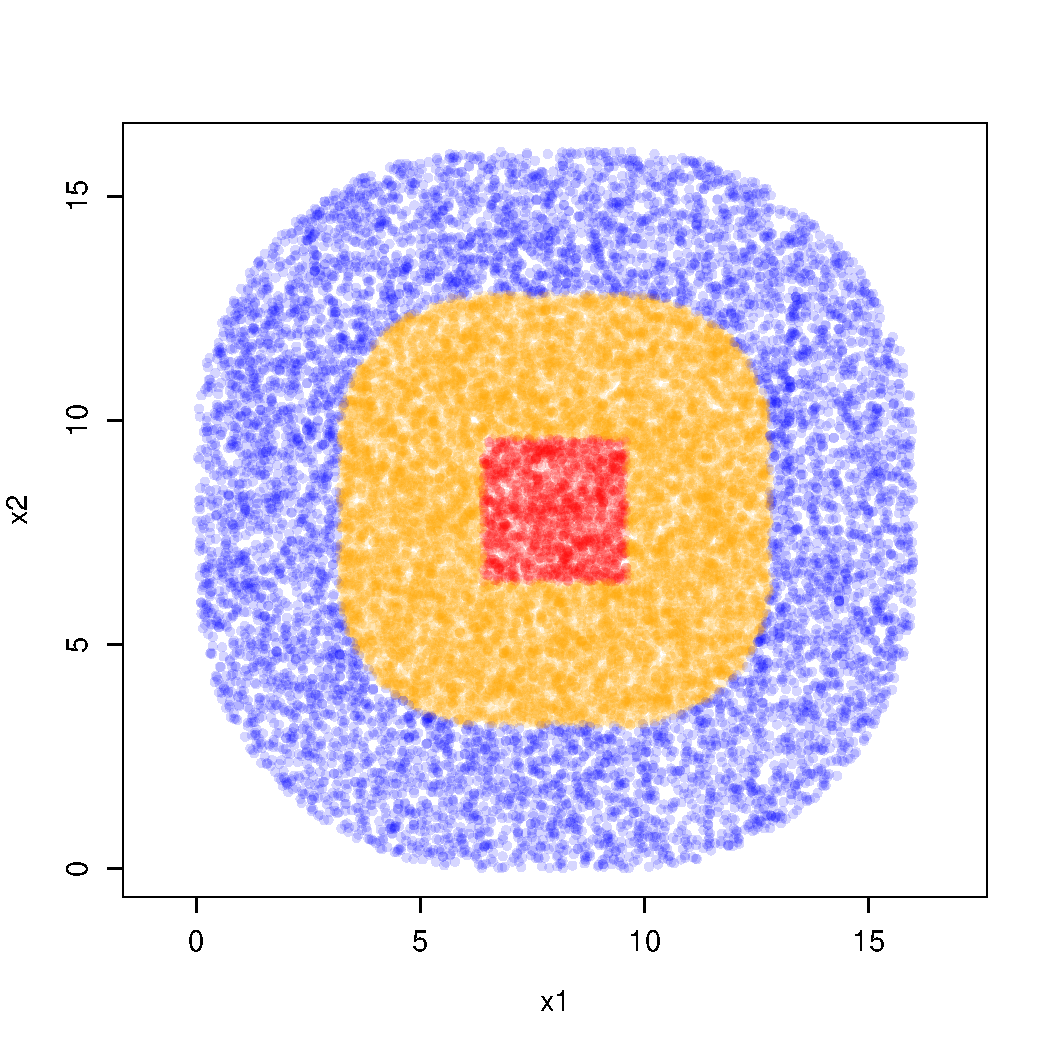
\includegraphics[width=0.32\textwidth]{example1plots/sample2}
  % \caption{}
  % \end{subfigure}
  % \begin{subfigure}{.33\linewidth}
  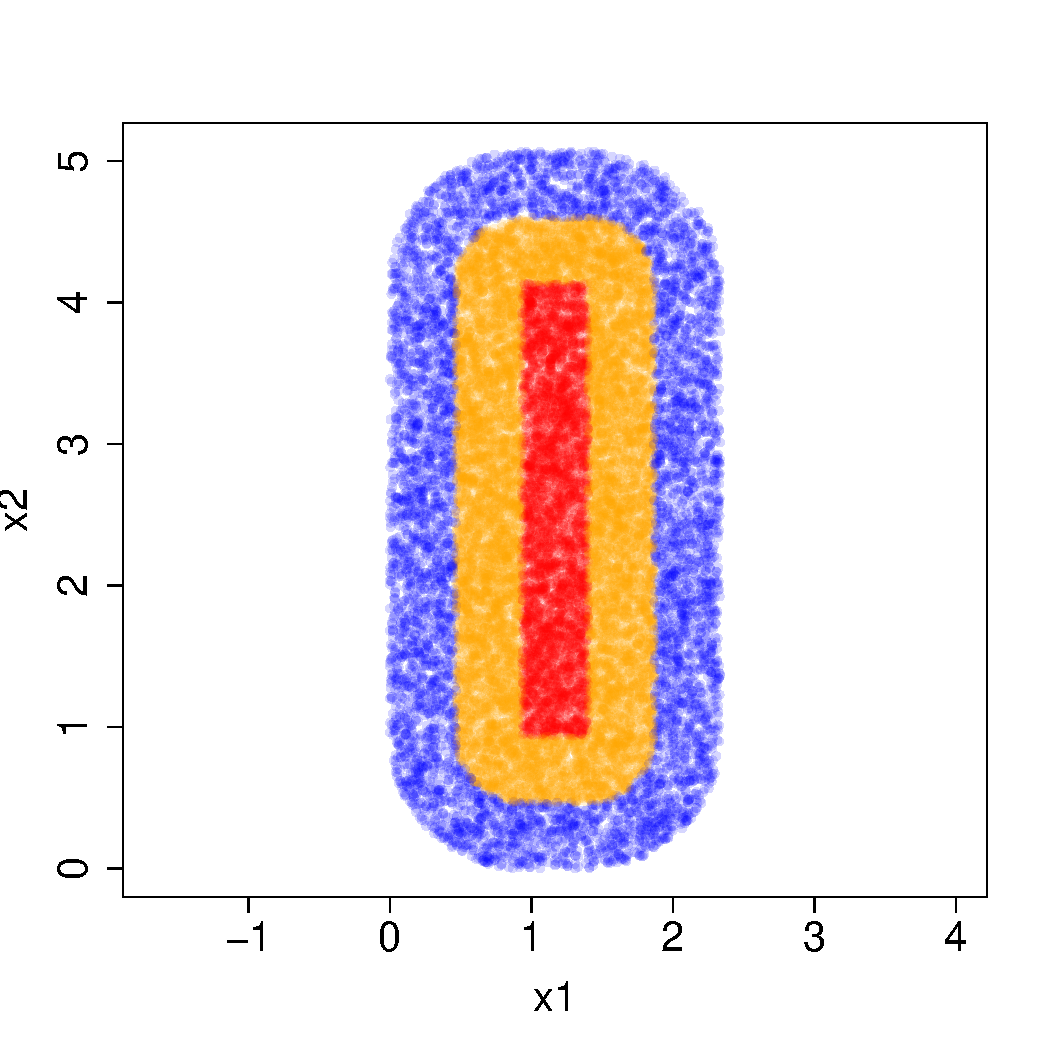
\includegraphics[width=0.32\textwidth]{example1plots/sample1}
  % \caption{}
  % \end{subfigure}
  % \begin{subfigure}{.33\linewidth}
  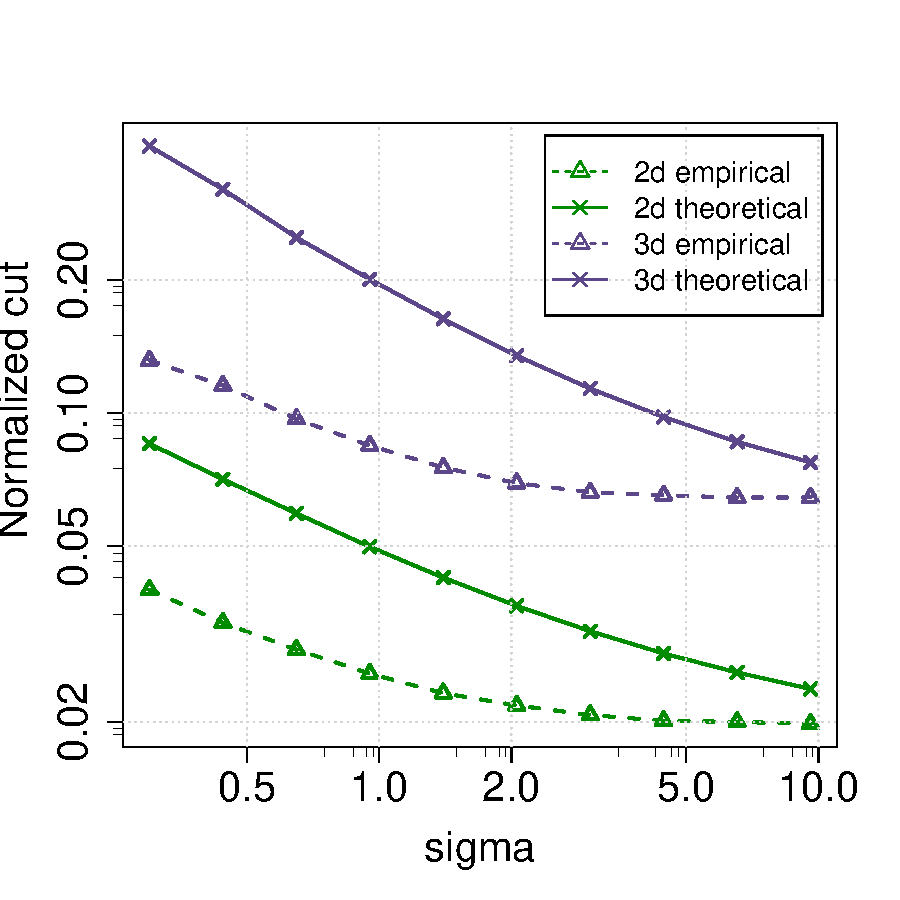
\includegraphics[width=0.32\textwidth]{example1plots/sigma_normalized_cut_plot}
  % \caption{}
  % \end{subfigure}
  
  % \begin{subfigure}{.33\linewidth}
  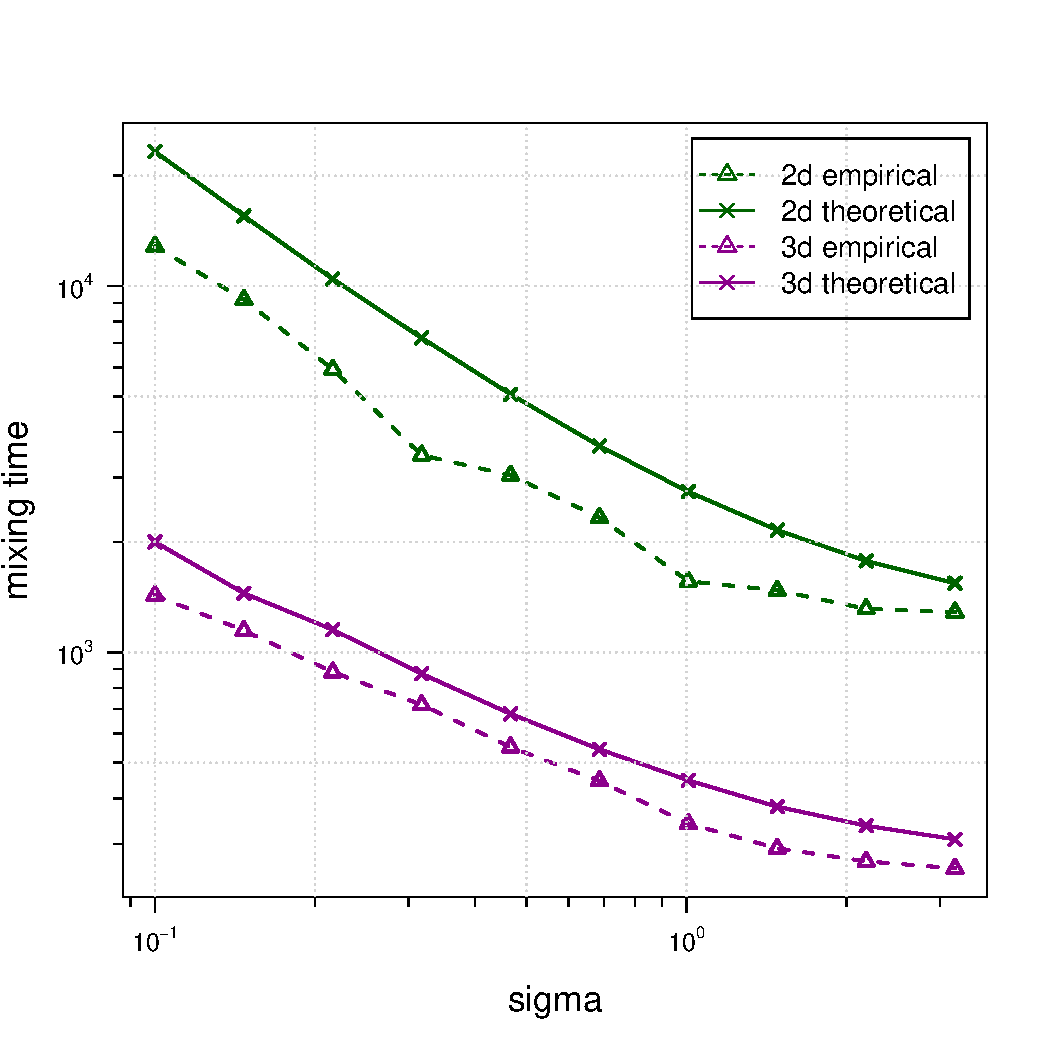
\includegraphics[width=0.32\textwidth]{example1plots/sigma_mixing_time_plot}
  % \caption{}
  % \end{subfigure}
  % \begin{subfigure}{.33\linewidth}
  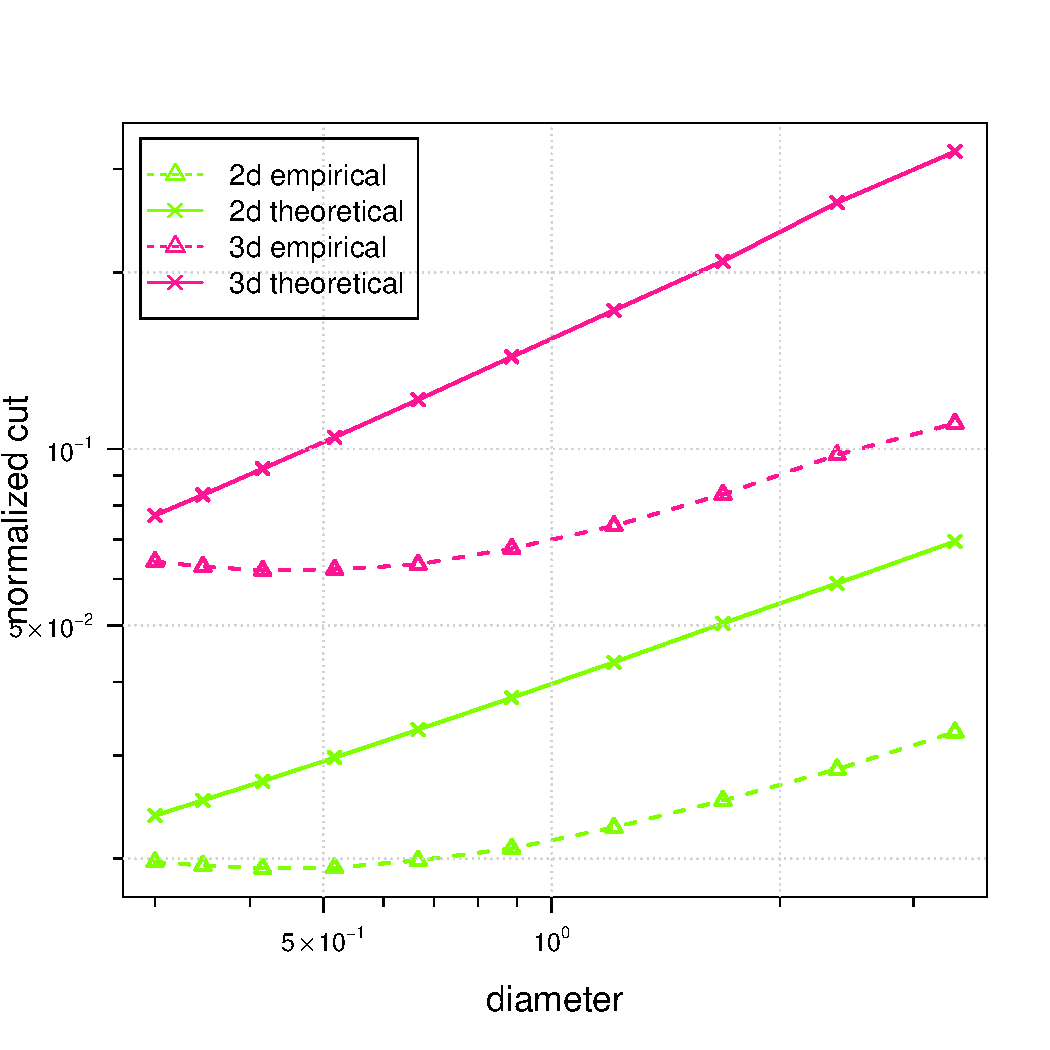
\includegraphics[width=0.32\textwidth]{example1plots/diameter_normalized_cut_plot}
  % \caption{}
  % \end{subfigure}
  % \begin{subfigure}{.33\linewidth}
  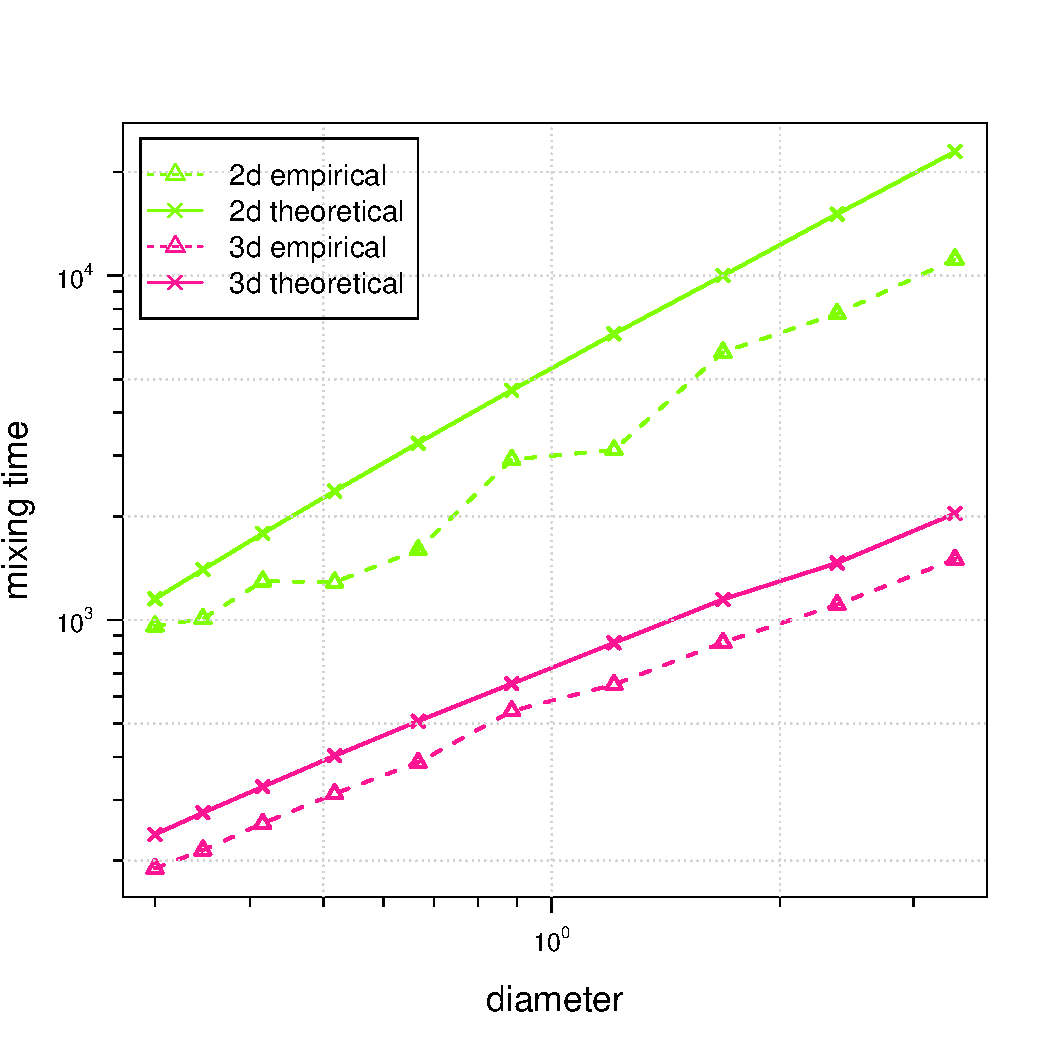
\includegraphics[width=0.32\textwidth]{example1plots/diameter_mixing_time_plot}
  % \caption{}
  % \end{subfigure}
  \caption{\it\small Top left and top middle: samples from a geometrically
    well- and poor-conditioned cluster. The points in $\Cset$ are colored in 
    red, points in $\Csig \setminus \Cset$ are colored in yellow, and the
    remaining points in blue. Other panels: empirical normalized cut and mixing
    time, as a function of $\sigma$ or $\rho$, versus their theoretical upper
    bounds.} 
  \label{fig:fig1}
%  \end{adjustbox}
\end{figure}

\paragraph{Validating theoretical bounds.}  We investigate the tightness of
Theorems \ref{thm: conductance_upper_bound} and \ref{thm:
  mixing_time_upper_bound} via simulation. Figure \ref{fig:fig1} compares our
upper bounds with the actual empirically-computed quantities \eqref{eqn:
  normalized_cut} and \eqref{eqn: mixing_time}, as we vary the diameter $\rho$
and thickness $\sigma$ of a cluster $\Cset$. The top left and top middle panels
display the resulting empirical clusters for two different values of
$\rho,\sigma$. 

The bottom left and bottom right panels assure that our mixing  
time upper bounds track closely the empirical mixing time, in both 2 and 3 
dimensions.\footnote{We rescaled all values of theoretical upper
  bounds by a constant, tto mask the effect of large universal constants
  in these bounds. Therefore only the comparison of slopes, rather than
  intercepts, is meaningful.} This provides empirical evidence that Theorem
\ref{thm: mixing_time_upper_bound} has the right dependency on both expansion
parameter $\sigma$ and diameter $\rho$. The story for the normalized cut panels
is less obvious. We remark that while, broadly speaking, the trends do not
appear to match, this gap between theory and empirical results seems largest
when $\sigma $ and $\rho$ are approximately equal. As the ratio $\rho/\sigma$
grows, the slopes of empirical and theoretical curves become more similar.

\paragraph{Empirical behavior of PPR.} In Figure \ref{fig:fig2}, to drive home
the main implications of Theorems \ref{thm:volume_ssd} and
\ref{thm: consistent_recovery_of_density_clusters}, we show the
behavior of PPR, normalized cut, and the density clustering algorithm of
\citet{chaudhuri2010} on the well known ``two moons'' dataset (with added 2d 
Gaussian noise), considered a prototypical success story for spectral clustering
algorithms. The first column shows the empirical density clusters $\Cset[\Xbf]$
and $\Cset'[\Xbf]$ for a particular threshold $\lambda$ of the density function; the 
second column shows the cluster recovered by PPR; the third column shows the
global minimum normalized cut, computed according to the algorithm of
\citet{szlam2010}; and the last column shows a cut of the density cluster tree
estimator of \citet{chaudhuri2010}.  We can see the degrading ability of PPR to
recover density clusters as the two moons become less well-separated. Of 
particular interest is the fact that PPR fails to recover one of the moons even
when normalized cut still succeeds in doing so. Additionally, we note that the Chaudhuri-Dasgupta algorithm succeeds even when both PPR and normalized cut fail.  While our main message was
that PPR recovers geometrically well-conditioned density clusters, it would be  
interesting to establish that it \emph{only} recovers such clusters, a direction
for future work.   

\begin{figure}
  \centering
  % \begin{adjustbox}{minipage=\linewidth}
  %   \begin{subfigure}{.24\linewidth}
  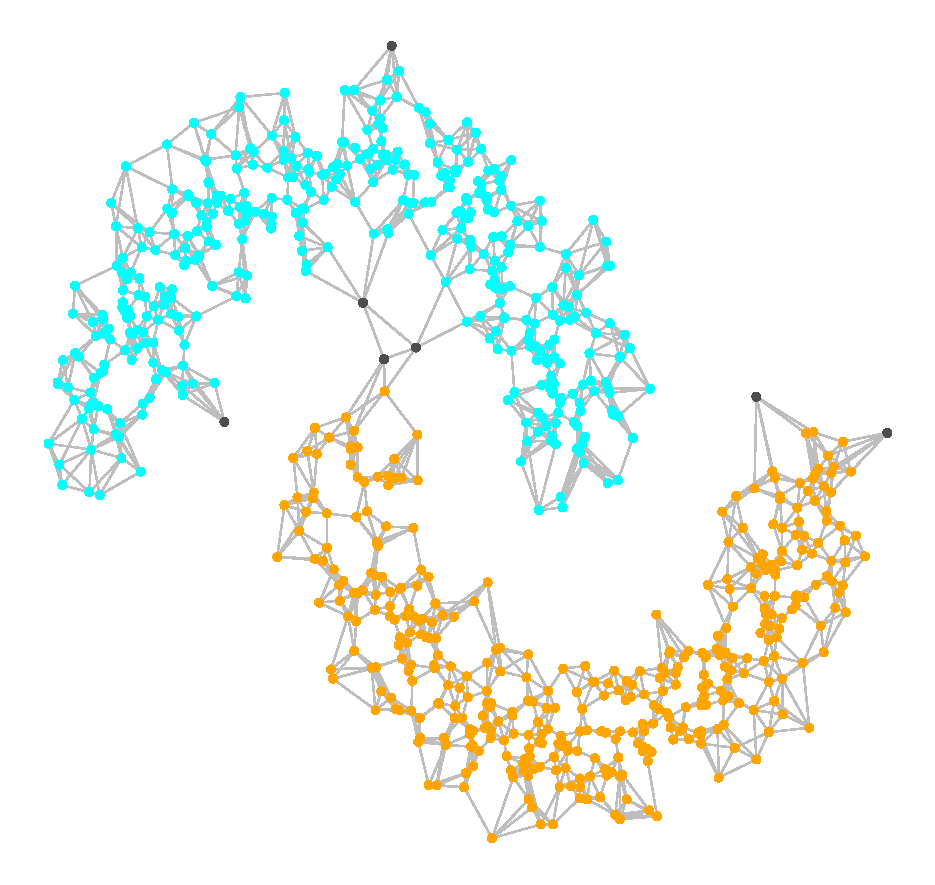
\includegraphics[width=0.24\textwidth,scale = .5]{example2plots/row1_true_density_cluster}
  % \caption{}
  % \end{subfigure}
  % \begin{subfigure}{.24\linewidth}
  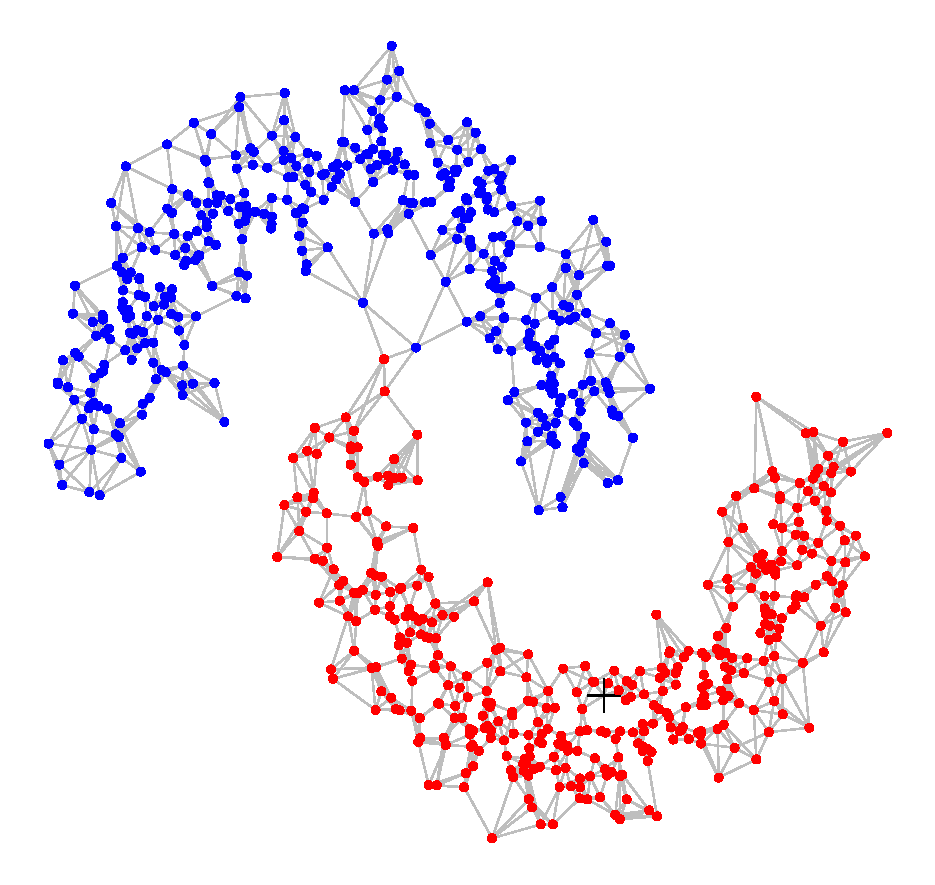
\includegraphics[width=0.24\textwidth]{example2plots/row1_ppr_cluster}
  % \caption{}
  % \end{subfigure}
  % \begin{subfigure}{.24\linewidth}
  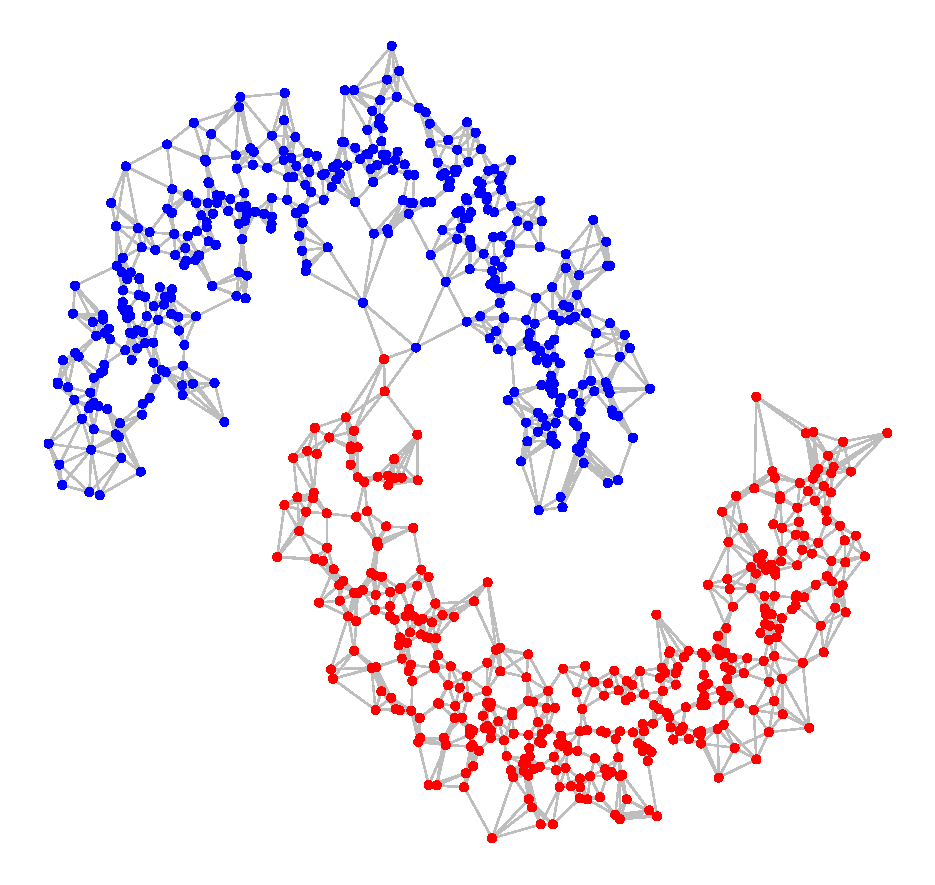
\includegraphics[width=0.24\textwidth]{example2plots/row1_conductance_cluster}
  % \caption{}
  % \end{subfigure}
  % \begin{subfigure}{.24\linewidth}
  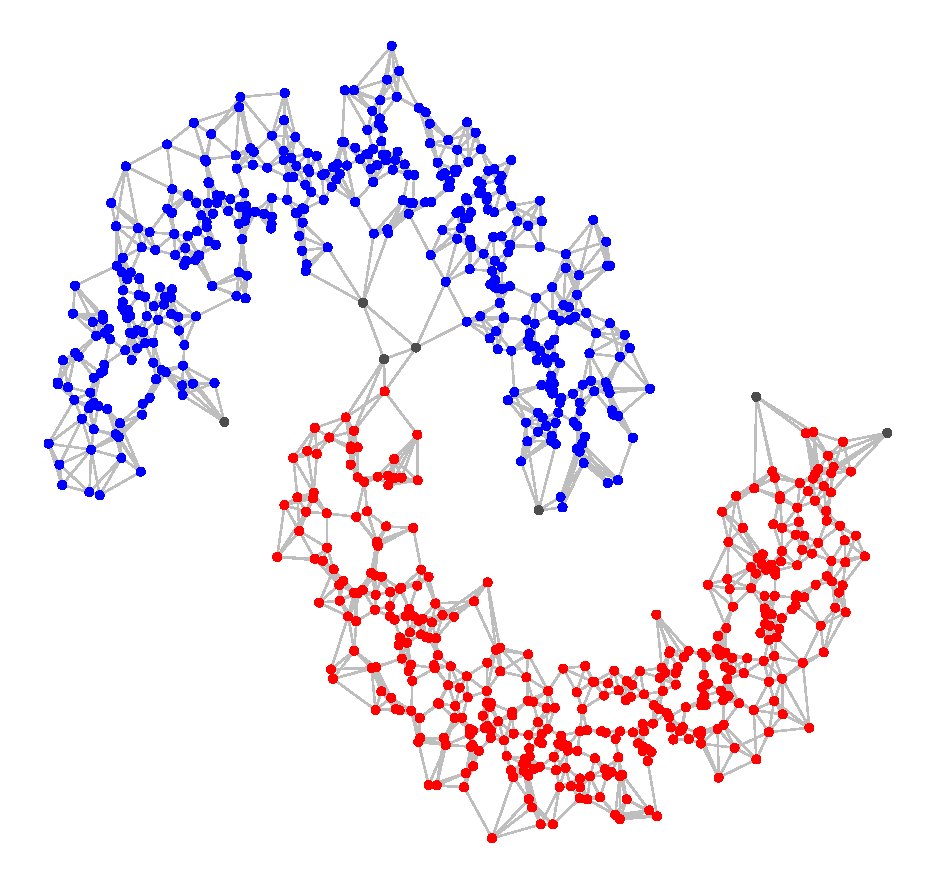
\includegraphics[width=0.24\textwidth]{example2plots/row1_density_cluster}
  % \caption{}
  % \end{subfigure}
  
  % \begin{subfigure}{.24\linewidth}
  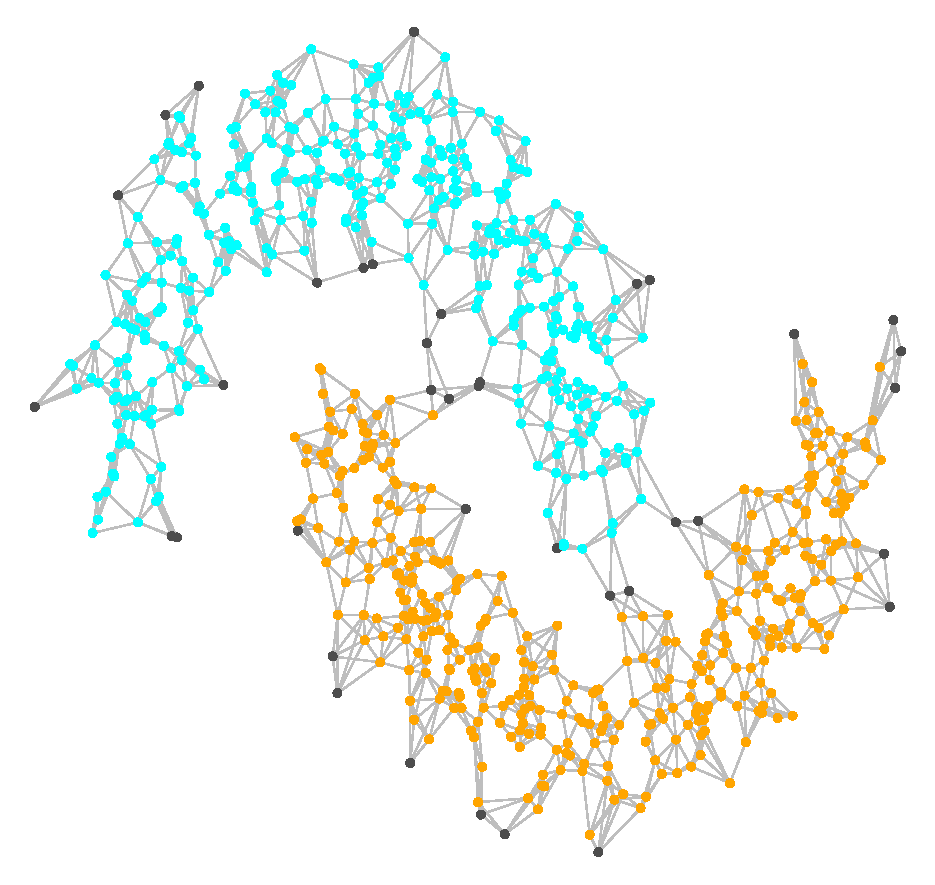
\includegraphics[width=0.24\textwidth]{example2plots/row2_true_density_cluster}
  % \caption{}
  % \end{subfigure}
  % \begin{subfigure}{.24\linewidth}
  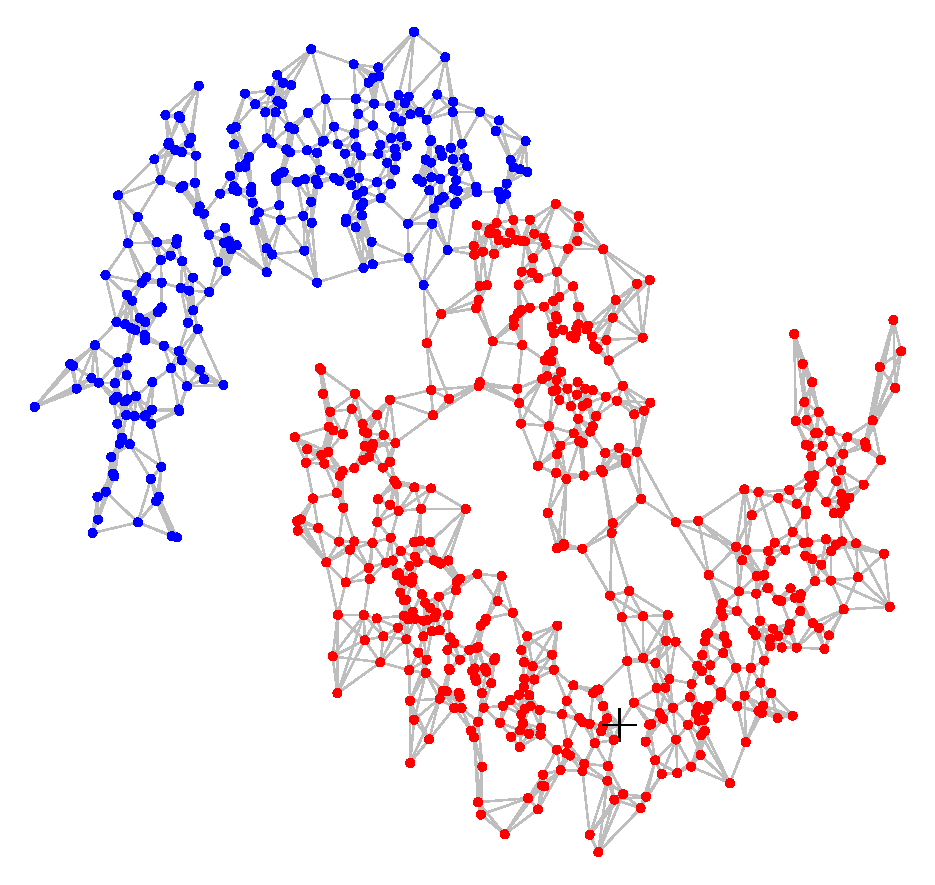
\includegraphics[width=0.24\textwidth]{example2plots/row2_ppr_cluster}
  % \caption{}
  % \end{subfigure}
  % \begin{subfigure}{.24\linewidth}
  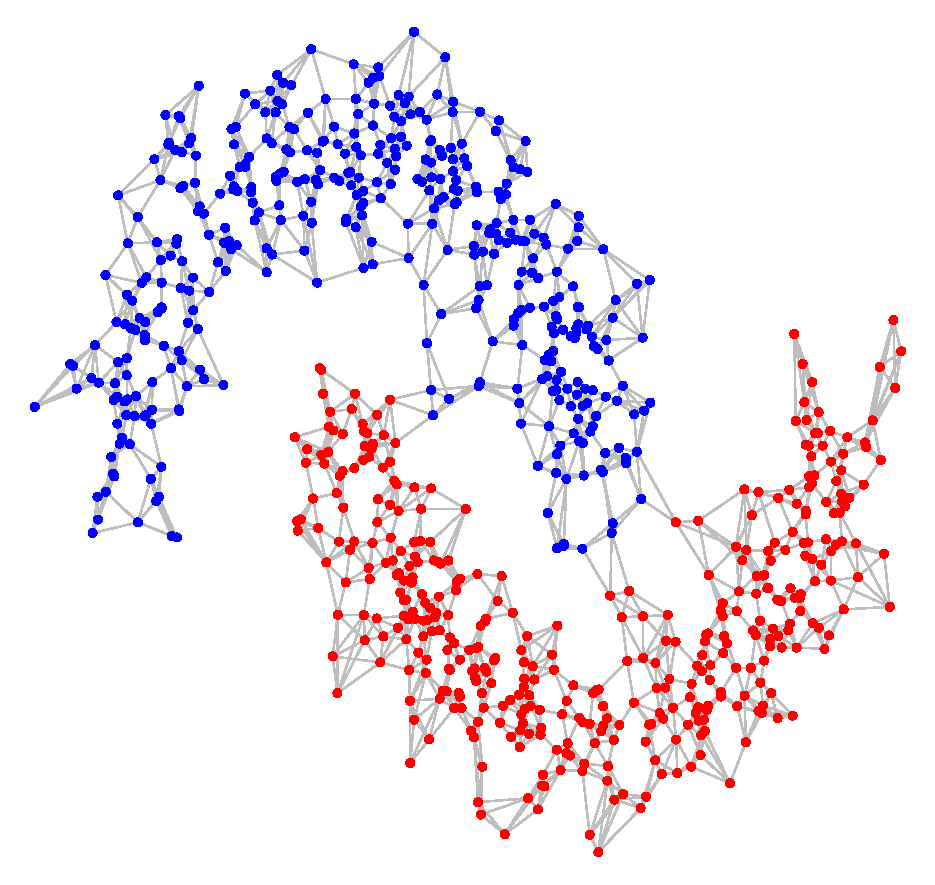
\includegraphics[width=0.24\textwidth]{example2plots/row2_conductance_cluster}
  % \caption{}
  % \end{subfigure}
  % \begin{subfigure}{.24\linewidth}
  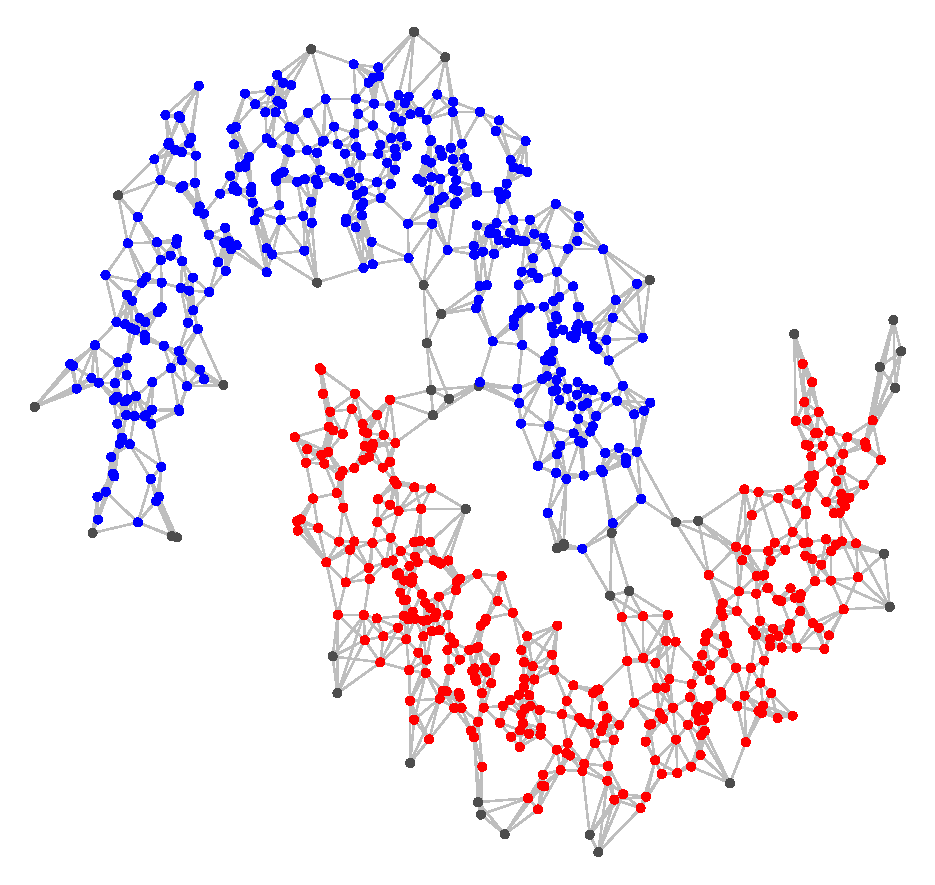
\includegraphics[width=0.24\textwidth]{example2plots/row2_density_cluster}
  % \caption{}
  % \end{subfigure}
  
  % \begin{subfigure}{.24\linewidth}
  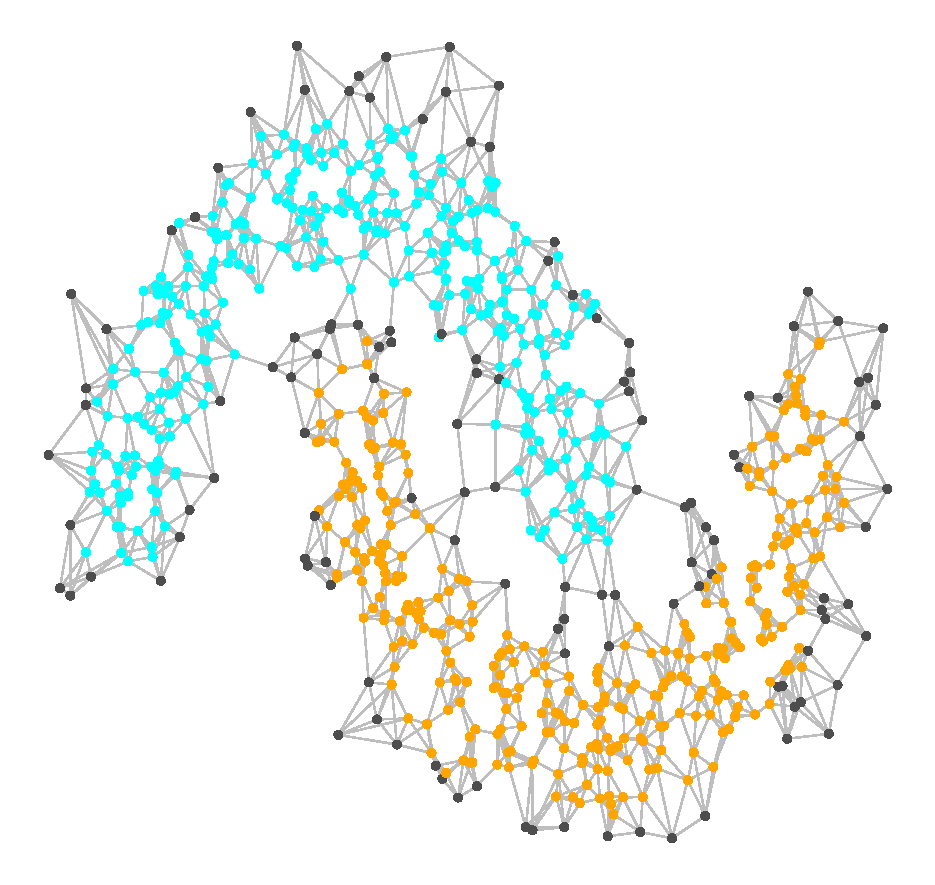
\includegraphics[width=0.24\textwidth]{example2plots/row3_true_density_cluster}
  % \caption{}
  % \end{subfigure}
  % \begin{subfigure}{.24\linewidth}
  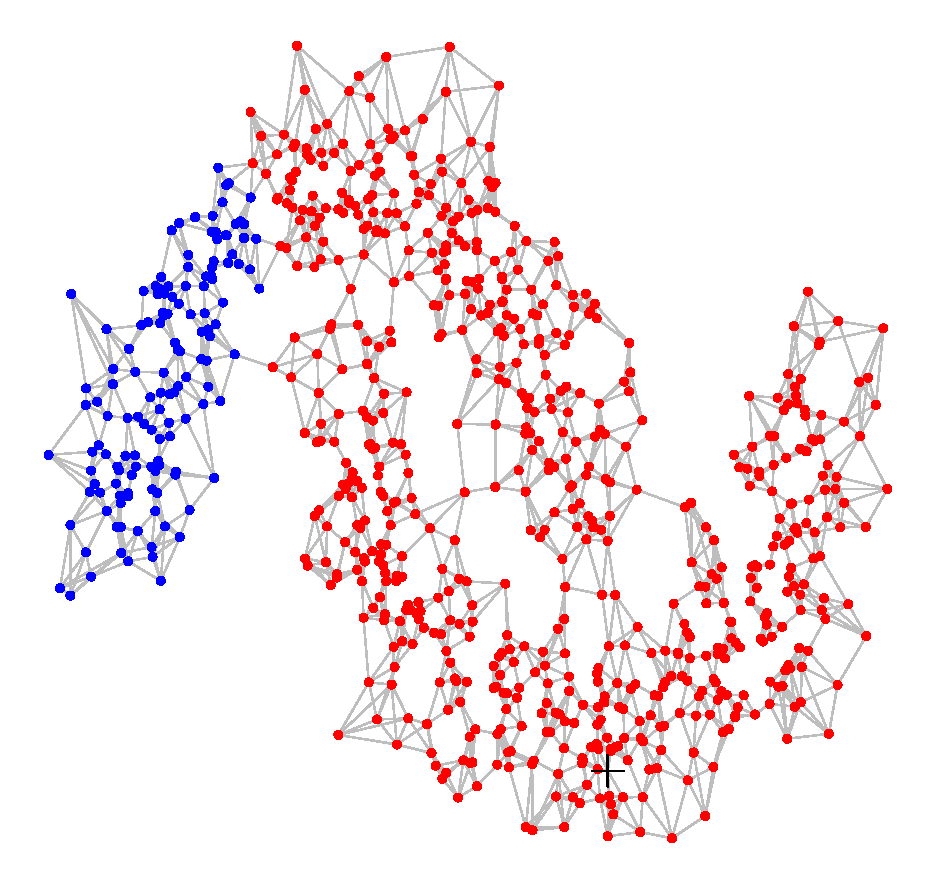
\includegraphics[width=0.24\textwidth]{example2plots/row3_ppr_cluster}
  % \caption{}
  % \end{subfigure}
  % \begin{subfigure}{.24\linewidth}
  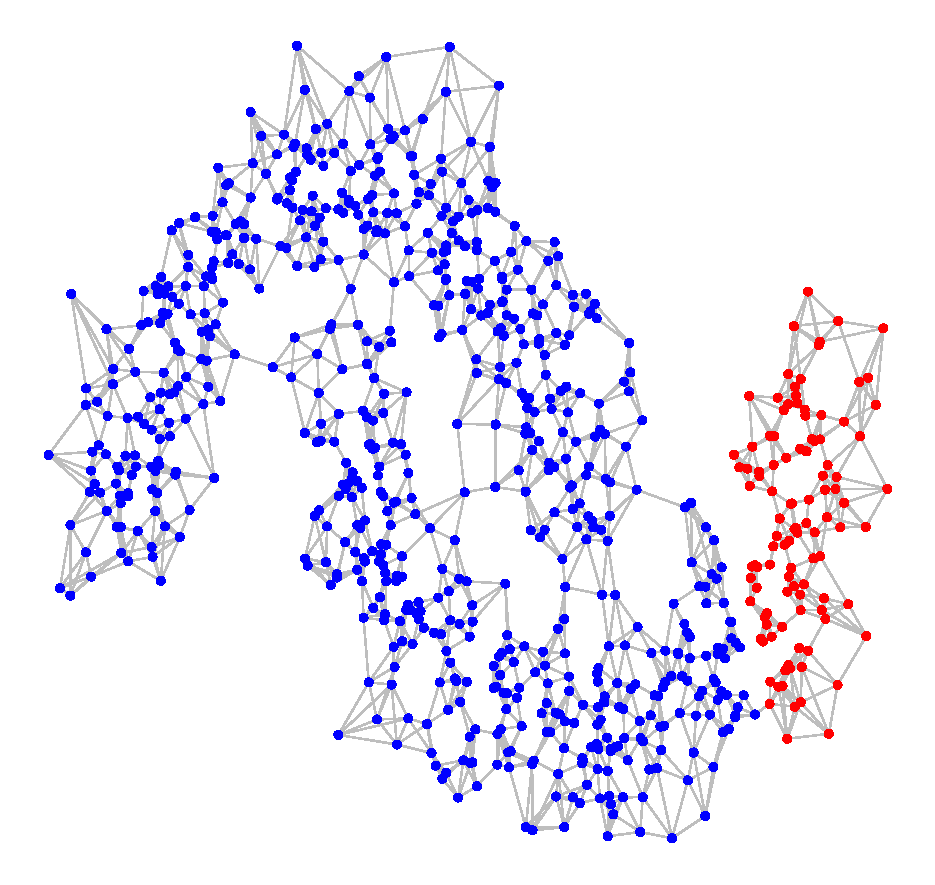
\includegraphics[width=0.24\textwidth]{example2plots/row3_conductance_cluster}
  % \caption{}
  % \end{subfigure}
  % \begin{subfigure}{.24\linewidth}
  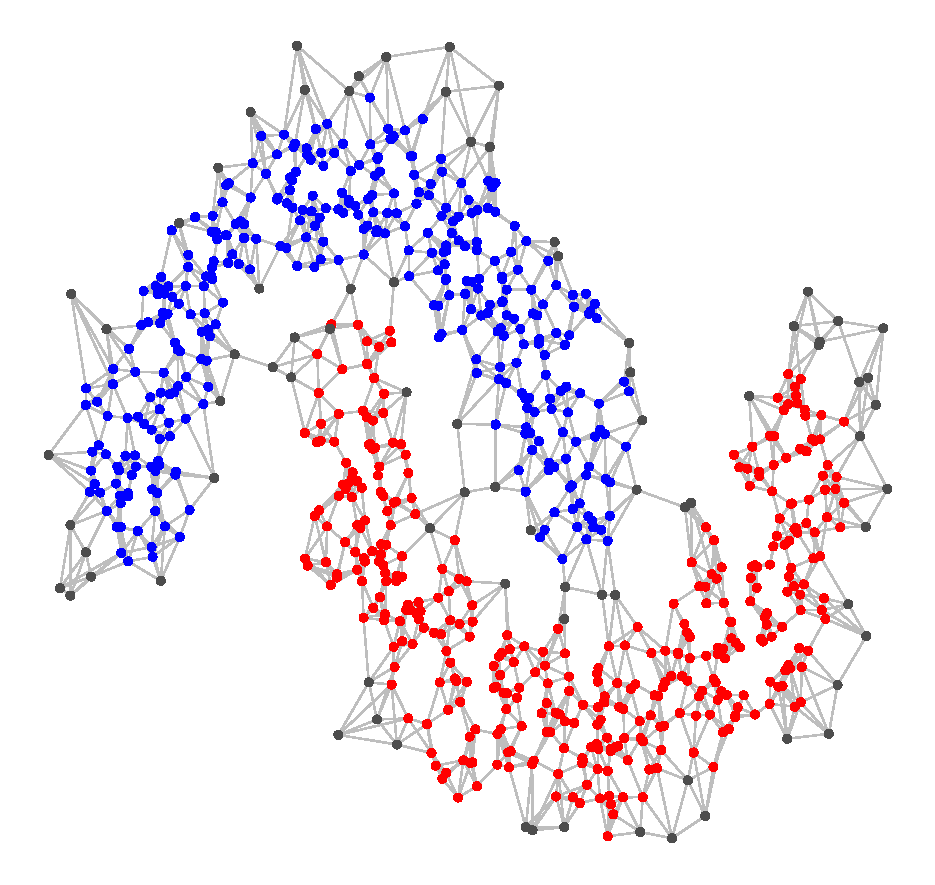
\includegraphics[width=0.24\textwidth]{example2plots/row3_density_cluster}
  % \caption{}
  % \end{subfigure}
  \caption{\it\small True density (column 1), PPR (column 2), normalized
    cut (column 3) and estimated density (column 4) clusters for 3 different 
    simulated data sets. Seed node for PPR denoted by a black cross.} 
  \label{fig:fig2}
  %\end{adjustbox}
\end{figure}

\section{Discussion}
\label{sec: discussion}

There are an almost limitless number of ways to define what the ``right''
clustering is. In this paper, we have considered one such notion---density upper
level sets---and have detailed a set of natural geometric criteria which, when 
appropriately satisfied, translate to provable bounds on estimation of the
cluster by PPR. We have also exhibited a hard case, showing that when a density cluster is sufficiently geometrically ill-conditioned, PPR may fail to recover it. Finally, we have empirically demonstrated the tightness of our analysis for reasonable sample sizes. 

\section{Acknowledgements}
SB is grateful to Peter Bickel, Martin Wainwright and Larry Wasserman for helpful and inspiring conversations. This work was supported in part by the NSF grant DMS-1713003.

\appendix

%In this supplement, we present proofs and experimental details for the article ``Local Spectral Clustering of Density Upper Level Sets''.
\section{Proof of Theorem \ref{thm: conductance_upper_bound}}
\label{sec: proof_of_theorem_1}

For notational ease, we let $\mathcal{S} \subseteq \Rd$ and write
\begin{align*}
\cut_{n,r}(\Csig[\Xbf]) = \cut(\Csig[\Xbf]; G_{n,r}),& ~ \cut_{\Pbb,r}(\Csig)= \frac{\mathbb{E}[\cut_{n,r}(\Csig[\Xbf])]}{2{n \choose 2}} \\
\vol_{n,r}(\Csig[\Xbf]) = \vol(\Csig[\Xbf]; G_{n,r}),& ~ \vol_{\Pbb,r}(\Csig)= \frac{\mathbb{E}[\vol_{n,r}(\Csig[\Xbf])]}{2{n \choose 2}}
\end{align*}
for the random variable and mean of cut size and volume, respectively. (Note that this definition of $\vol_{\Pbb,r}(\Sset)$ agrees with that of~\eqref{eqn:volume}). 

With this notation in place, the goal of Theorem~\ref{thm: conductance_upper_bound} is to show that for a universal constant $c_1 > 0$,
\begin{align*}
\Phi_{n,r}(\Csig[\Xbf]) := \frac{\cut_{n,r}(\Csig[\Xbf])}{\min\{\vol_{n,r}(\Csig[\Xbf]), \vol_{n,r}((\Rd \setminus \Csig)[\Xbf])\}} \leq c_1 \frac{d}{\sigma}
    \frac{\lambda}{\lambda_{\sigma}} \frac{(\lambda_{\sigma} -
      c_0\frac{r^{\gamma}}{\gamma+1})}{\lambda_{\sigma}}
\end{align*}
with probability at least $1 - 3\exp\{-nc_1(\Pbb,r)\}$.

The proof of this theorem follows essentially from two technical Lemmas. 
Lemma~\ref{lem:ball_bounds_in_probability} relates the terms in the numerator and denominator of $\Phi_{n,r}(\Csig[\Xbf])$ to their expected values. We restate the conclusions of this Lemma: for any $\delta > 0$,
\begin{align}
\frac{\cut_{n,r}(\Csig[\Xbf])}{2{n \choose 2}} \leq (1 + \delta)\cut_{\Pbb,r}(\Csig) &, \quad \frac{\vol_{n,r}(\Csig[\Xbf])}{2{n \choose 2}} \geq (1 - \delta)\vol_{\Pbb,r}(\Csig) \nonumber \\ \frac{\vol_{n,r}((\Rd \setminus \Csig)[\Xbf])}{2{n \choose 2}}& \geq (1 - \delta)\vol_{\Pbb,r}(\Rd \setminus \Csig) \label{eqn: conductance_upper_bound_pf1}
\end{align}
with probability at least 
\begin{align*}
1 - & \exp\set{-n \delta^2 (\cut_{\Pbb,r}(\Csig))^2} - \exp\set{-n \delta^2 (\vol_{\Pbb,r}(\Csig))^2} - \exp\set{-n \delta^2 (\vol_{\Pbb,r}(\Rd\setminus \Csig))^2} \\
& \geq 1 - 3\exp\set{-n \delta^2 (\cut_{\Pbb,r}(\Csig))^2}.
\end{align*} 
We note that as a consequence of~\ref{asmp: bounded_volume} we have that $\vol_{\Pbb,r}(\Rd \setminus \Csig)  \geq \vol_{\Pbb,r}(\Csig)$, so it will suffice to lower bound $\vol_{\Pbb,r}(\Csig)$ (since a lower bound for $\vol_{\Pbb,r}(\Rd \setminus \Csig)$ follows).
The following result provides upper and lower bounds on the expected values $\cut_{\Pbb,r}(\Csig)$ and $\vol_{\Pbb,r}(\Csig)$ respectively:
\begin{lemma}
	\label{lem: expected_density_cut}\label{lem: expected_density_volume}
	Under the setup and conditions of Theorem \ref{thm: conductance_upper_bound}, and for any $0 < r \leq \sigma/2d$,
	\begin{align}
	\cut_{\Pbb,r}(\Csig) &\leq \frac{4 d \nu_d r^{d+1} \lambda}{\sigma} \left(\lambda_{\sigma} - c_0\frac{r^{\gamma}}{\gamma + 1}\right) \nu(\Csig), \label{eqn:claim_one} \\
	\vol_{\Pbb,r}(\Csig) &\geq \frac{12}{25} \lambda_{\sigma}^2 \nu_d r^d \nu(\Csig).\label{eqn:claim_two}
	\end{align}
\end{lemma}
Taking Lemma~\ref{lem: expected_density_cut} and \eqref{eqn: conductance_upper_bound_pf1} as given we can now complete the proof of the theorem. We lower bound $\Phi_{n,r}(\Csig[\Xbf])$ as follows:
\begin{equation*}
\Phi_{n,r}(\Csig[\Xbf]) \leq \frac{(1 + \delta)\cut_{\Pbb,r}(\Csig)}{(1 - \delta)\vol_{\Pbb,r}(\Csig)} \leq \frac{25(1 + \delta)d \nu_d r \lambda \left(\lambda_{\sigma} - c_0\frac{r^{\gamma}}{\gamma + 1}\right)}{3(1 - \delta) \sigma \lambda_{\sigma}^2}.
\end{equation*}
Plugging in $\delta = \frac{1}{2}$, the theorem is satisfied by choosing constants $c_1 = 50$ and $c_1(\Pbb,r) = \frac{1}{4}(\cut_{\Pbb,r}(\Csig))^2$. 

\subsection{Proof of Lemma~\ref{lem: expected_density_cut}}
We write $\Pbb(\Aset) = \int_{\Aset} f(x) dx$ for measurable $\Aset \subseteq \Rd$.
We 
let $\Csigr := \set{x: 0 < \dist(x, \Csig) < r}$, where $\Csig$ is as in Theorem \ref{thm: conductance_upper_bound}. 
Our goal will be to upper bound $\cut_{\Pbb,r}(\Csig)$ by a term that depends on the probability mass $\Pbb(\Csigr)$, 
and the bulk of our technical effort will be devoted to showing the following upper bound on $\Pbb(\Csigr)$:
%Lemma \ref{lem: expected_number_boundary_points} involves the bulk of the technical effort required to prove Theorem \ref{thm: conductance_upper_bound}; it will be necessary to bound the expected cut size of $\Csig[\Xbf]$ in $G_{n,r}$. 
\begin{lemma}
	\label{lem: expected_number_boundary_points}
	Under the conditions of Theorem \ref{thm: conductance_upper_bound}, and for any $0 < r \leq \sigma/2d$,
	\begin{equation*}
	\Pbb(\Csigr) \leq \frac{2dr}{\sigma} \left(\lambda_{\sigma} - c_0\frac{r^{\gamma}}{\gamma + 1}\right) \nu(\Csig)
	\end{equation*}	
\end{lemma}
\noindent Define the \emph{uniform local conductance} $\ell_{\nu,r}(u)$ to be
\begin{equation*}
\ell_{\nu,r}(u) = \nu\bigl(\Csig \cap B(u,r)\bigr).
\end{equation*}
In order to lower bound $\vol_{\Pbb,r}(\Csig)$ we will show the following lower bound on the uniform local conductance:
\begin{lemma}
	\label{lem: local_conductance}
	Let $u \in \Csig$. Then, for any $0 < r \leq \frac{\sigma}{2\sqrt{d}}$,
	\begin{equation*}
	\ell_{\nu,r}(u) \geq \frac{6}{25} \nu_d r^d.
	\end{equation*}
\end{lemma}
Taking these two results as given we can now prove each of the two claims~\eqref{eqn:claim_one} and~\eqref{eqn:claim_two} in turn.
\paragraph{Proof of Claim~\eqref{eqn:claim_one}: } For each $i,j$ such that $i \neq j$, we can write 
\begin{equation*}
\cut_{\Pbb,r}(\Csig) =  \Pbb(x_i \not\in \Csig, x_j \in \Csig, \norm{x_i - x_j} \leq r).
\end{equation*}
Writing this as an integral, we have
\begin{align*}
\cut_{\Pbb,r}(\Csig) & = \int_{\Rd \setminus \Csig} f(x) \Pbb\bigl(B(x,r) \cap \Csig\bigr) \dx \\
& = \int_{\Csigr} f(x) \Pbb\bigl(B(x,r) \cap \Csig\bigr) \dx \\
& \leq \nu_d r^d \lambda  \int_{\Csigr} f(x) \dx = \nu_d r^d \lambda \Pbb(\Csigr).
\end{align*}
where the inequality follows from \ref{asmp: low_noise_density}, which implies $f(x) \leq \lambda$ for $x \in \Csig \setminus \Cset$. Then, upper bounding the integral using Lemma \ref{lem: expected_number_boundary_points} gives the final result.


%\subsection{Proof of Lemma~\ref{Z}}
\paragraph{Proof of Claim~\eqref{eqn:claim_two}: }  For each $i,j$ such that $i \neq j$, we can write 
\begin{equation*}
\vol_{\Pbb,r}(\Csig) = \Pbb(x_i \in \Csig, x_j \in B(x_i,r))
\end{equation*}
Writing this as an integral, we have
\begin{align*}
\vol_{\Pbb,r}(\Csig) & = 2 \int_{\Csig} f(x) \Pbb(B(x,r)) \dx \\
& \geq 2 \int_{\Csig} f(x) \Pbb(B(x,r) \cap \Csig) \dx
\end{align*}
whence the claim then follows by Lemma \ref{lem: local_conductance}.
It remains to prove Lemmas~\ref{lem: expected_number_boundary_points} and~\ref{lem: local_conductance}, and we turn our attention to this next.
\subsection{Proof of Lemma~\ref{lem: expected_number_boundary_points}}
The proof of this Lemma relies on certain volume estimates whose statement and proof we defer to Appendix~\ref{sec: volume_estimates}.
	We partition $\Csigr$ into slices based on distance from $\Csig$ as follows: for $k \in \N$,
	\begin{equation*}
	\mathcal{T}_{i,k} = \set{x \in \Csigr: t_{i,k} < \frac{\dist(x, \Csig)}{r} \leq t_{i+1,k}}, ~~ \Csigr = \bigcup_{i = 0}^{k-1} \mathcal{T}_{i,k},
	\end{equation*}
	where $t_{i,k} = i/k$ for $i = 0, \ldots, k - 1$. As a result, for any $k \in \mathbb{N}$,
	\begin{equation}
	\label{eqn: partition_ub}
	\Pbb(\Csigr) = \int_{\Csigr} f(x) \dx = \sum_{i = 0}^{k-1} \int_{\mathcal{T}_{i,k}} f(x) \dx \leq \sum_{i = 0}^{k-1} \nu(\mathcal{T}_{i,k}) \max_{x \in \mathcal{T}_{i,k}} f(x).
	\end{equation}
	Assumptions~\ref{asmp: bounded_density} and \ref{asmp: low_noise_density} imply the upper bound
	\begin{equation*}
	\max_{x \in \mathcal{T}_{i,k}} f(x) \leq \lambda_{\sigma} - c_0(rt_{i,k})^{\gamma},
	\end{equation*}
	and writing
	\begin{equation*}
	\nu(\mathcal{T}_{i,k}) = \nu(\Csig + rt_{i+1,k}B) - \nu(\Csig + rt_{i,k}B) =: \nu_{i+1,k} - \nu_{i,k},
	\end{equation*}
	we have
	\begin{align}
	\label{eqn: telescoping_sum}
	\sum_{i = 0}^{k-1} \nu(\mathcal{T}_{i,k}) \max_{x \in \mathcal{T}_{i,k}} f(x) & \leq \sum_{i = 0}^{k-1} \biggl\{ \nu_{i+1,k} - \nu_{i,k} \biggr\} \biggl( \lambda_{\sigma} - c_0(rt_{i,k})^{\gamma} \biggr) \nonumber \\
	& = \underbrace{\sum_{i = 1}^{k} 
	\nu_{i,k} \biggl( \left[\lambda_{\sigma} - c_0(rt_{i-1,k})^{\gamma}\right] -  \left[\lambda_{\sigma} - c_0(rt_{i,k})^{\gamma}\right]\biggr)}_{:= \Sigma_k} + \underbrace{\biggl(\nu_{k,k}\left[\lambda_{\sigma} - c_0r^{\gamma}\right] - \nu_{1,k}\lambda_{\sigma} \biggr)}_{:= \xi}
	\end{align}
	where the second equality comes from rearranging terms in the sum.
	
	% AJG 5/14/19: This argument makes sense, correct?
	We first consider the term $\Sigma_k$. $\Cset$ has finite diameter by Assumption~\ref{asmp: bounded_density}, as otherwise $\int_{\Csig} f(x) dx = \infty$. Letting $\overline{\Cset}$ be the closure of $\Cset$, we observe that $\overline{\Csig} = \overline{\Cset} + \sigma B$, and moreover for any $\delta > 0$, $\nu(\overline{\Csig} + \delta B) = \nu(\Csig + \delta B)$ (as the boundary $\partial(\Csig + \delta B)$ is Lipschitz and therefore has measure zero). As a result, for each $t_{i,k}, i = 1, \ldots,k$ we may apply Lemma \ref{lem: expansion_volume} to $\overline{\Cset}$ and obtain
	\begin{equation}
	\label{eqn: slice_volume_bound}
	\nu_{i,k} = \nu(\Csig + rt_{i,k}B) \leq \nu(\Csig)\left(1 + \frac{rt_{i,k}}{\sigma}\right)^d
	\end{equation}
	which in turn gives
	\begin{align}
	\Sigma_k & \leq c_0\nu(\Csig) r^\gamma \sum_{i = 1}^{k} \left(1 + \frac{ rt_{i,k}}{\sigma}\right)^d \biggl( (t_{i,k})^{\gamma} - (t_{i-1,k})^{\gamma}\biggr) \nonumber \\
	& = c_0\nu(\Csig) r^\gamma \sum_{i = 1}^{k} \left(1 + \frac{ru_{i,k}^{1/\gamma}}{\sigma}\right)^d ( u_{i,k} - u_{i,k-1}).~~~~~~~~~~~~~~ (\text{substituting}~u_{i,k} := t_{i,k}^{\gamma}) \label{eqn: Sigmak_riemann_sum}
	\end{align}
	The expression in~\eqref{eqn: Sigmak_riemann_sum} is a Riemann sum, and taking the limit as $k \to \infty$ we obtain
	\begin{align}
	\lim_{k \to \infty} c_0\nu(\Csig) r^\gamma \sum_{i = 1}^{k} \left(1 + \frac{ru_{i,k}^{1/\gamma}}{\sigma}\right)^d ( u_{i,k} - u_{i,k-1}) & = c_0\nu(\Csig) r^\gamma \int_{0}^{1} \left(1 + \frac{r u^{1/\gamma}}{\sigma}\right)^{d} du \nonumber \\
	& \overset{\text{(i)}}{\leq} c_0\nu(\Csig) r^\gamma \int_{0}^{1} \left(1 + \frac{2 d r u^{1/\gamma}}{\sigma}\right) du \nonumber \\
	& = c_0\nu(\Csig) r^\gamma \left(1 + \gamma \frac{2 d r}{(\gamma + 1)\sigma}\right). \label{eqn: Sigmak_integral}
	\end{align}
	where $\text{(i)}$ follows from the upper bound in Lemma \ref{lem: Taylor_series} in light of the fact $r \leq \sigma / 2d$. 
	
	An upper bound on $\xi$ follows from largely the same logic, although it does not involve integration:
	\begin{align}
	\xi & \overset{\text{(ii)}}{\leq} \nu(\Csig) \biggl\{ \left(1 + \frac{ r}{\sigma}\right)^d(\lambda_{\sigma} - c_0r^{\gamma}) - \lambda_{\sigma} \biggr\} \nonumber \\
	& \overset{\text{(iii)}}{\leq} \nu(\Csig) \biggl\{ \left(1 + \frac{2d r}{\sigma}\right)(\lambda_{\sigma} - c_0r^{\gamma}) - \lambda_{\sigma} \biggr\} = \nu(\Csig) \biggl\{ \frac{2dr}{\sigma}(\lambda_{\sigma} - c_0r^{\gamma}) - c_0 r^{\gamma} \biggr\}. \label{eqn: xi_ub}
	\end{align}
	where $\text{(ii)}$ follows from \eqref{eqn: slice_volume_bound}, and $\text{(iii)}$ from Lemma \ref{lem: Taylor_series}. As the bounds in \eqref{eqn: partition_ub} and \eqref{eqn: telescoping_sum} hold for all $k$, these along with \eqref{eqn: Sigmak_integral} and \eqref{eqn: xi_ub} imply the desired result.



%\subsection{Proof of Lemma~\ref{lem: expected_number_boundary_points}}



\subsection{Proof of Lemma~\ref{lem: local_conductance}}
The proof of this result relies on estimates of the volume of spherical caps which we defer to Appendix~\ref{sec:caps}.
	Since $u \in \Csig$ there exists $x \in \Cset$ such that $u \in B(x, \sigma)$, and as $B(x,\sigma) \subseteq \Csig$,
	\begin{equation*}
	\nu\bigl(B(u, r) \cap B(x, \sigma)\bigr) \leq \nu\bigl(B(u, r) \cap \Csig \bigr)
	\end{equation*}
	Without loss of generality, let $\norm{u - x} = \sigma$; it is not hard to see that if $\norm{u - x} < \sigma$, the volume of the overlap will only grow. Then, since $\norm{u  - x} = \sigma$, $B(u, r) \cap B(x, \sigma)$ contains a spherical cap of radius $r$ and height
	\begin{equation*}
	h = r - r^2/2\sigma = r \left( 1 - \frac{r}{2 \sigma} \right)
	\end{equation*}	
	which by Lemma \ref{lem: volume_of_spherical_cap} has volume
	\begin{equation*}
	\nu_{\text{cap}} = \frac{1}{2} \nu_d r^d I_{1 - \alpha}\left( \frac{d + 1}{2}  ,\frac{1}{2}\right)
	\end{equation*}
	with $\alpha = 1 - \frac{2rh - h^2}{r^2} = \frac{r^2}{4 \sigma^2} \leq \frac{1}{16d}$. 
	By Lemmas \ref{lem: beta_integral} (applied with $t = 1$) and \ref{lem: beta_function},
	\begin{align*}
	I_{1 - \alpha}\left( \frac{d + 1}{2}  ,\frac{1}{2}\right) & \geq 1 - \frac{\Gamma\bigl(\frac{d}{2}+ 1\bigr)}{\Gamma\bigl(\frac{d + 1}{2}\bigr) \Gamma\bigl(\frac{1}{2}\bigr)} \frac{3}{4\sqrt{d}} \\
	& \geq 1 - \frac{3}{4}\sqrt{\frac{d+2}{\pi d}} \geq 1 - \frac{3}{4}\sqrt{\frac{3}{2 \pi}}.
	\end{align*}


\subsection{Volume Estimates}
\label{sec: volume_estimates}
%\section{Proofs}
%
%Subsections \ref{sec: volume_estimates} - \ref{sec: proof_of_theorem_1} detail the proof for Theorem \ref{thm: conductance_upper_bound}. In subsections \ref{sec: mixing_time_on_graphs} and \ref{sec: proof_of_proposition_tv_mixing_time}, we establish some results regarding mixing time over general graphs. The proof of Theorem \ref{thm: mixing_time_upper_bound} is then provided in subsections \ref{sec: population_conductance_function} - \ref{sec: proof_of_theorem_mixing_time}. Section~\ref{sec: concentration} gives some general concentration results we use throughout, before we finish with the proofs of Theorems \ref{thm: misclassification_rate} and \ref{thm: consistent_recovery_of_density_clusters}, and the statement and proof of our results regarding the a\pprspace vector (Corollary \ref{cor: appr}), in subsections \ref{sec: proof_of_misclassification_rate} - \ref{sec: linalg}.

%\subsection{Volume estimates}


We begin by recalling some notation. We let $\Aset \subseteq \Reals^d$, and for $\sigma \geq 0$, write $\sigma B := B(0,\sigma) = \set{x \in \Rd: \norm{x} \leq \sigma}$ for the closed ball of radius $\sigma$ centered at the origin (and let $B^{\circ}(0,\sigma)$ denote the corresponding open ball). Let $\Asig = \Aset + \sigma B$ be the direct sum of $\Aset$ and $\sigma B$, $\Asig = \set{z = x + y: x \in \Aset, y \in \sigma B}$. Recall that we use $\nu$ for Lebesgue measure, and $\nu_d = \nu(B)$ for $B = (0,1)$. 

Lemma \ref{lem: expansion_volume} provides a bound on the ratio $\nu(\Csig + r B) / \nu(\Csig)$, an important intermediate quantity in bounding the ratio $\cut(\Csig[\Xbf]; G_{n,r})/\vol(\Csig[\Xbf]; G_{n,r})$. 

\begin{lemma}
	\label{lem: expansion_volume}
	If $\Aset$ is closed and bounded, then for any $\delta > 0$,
	\begin{equation}
	\label{eqn: expansion_volume}
	\nu(\Asig + \delta B) \leq \left(1 + \frac{\delta}{\sigma}\right)^d \nu(\Asig).
	\end{equation}
\end{lemma}
\begin{proof}
	We will show that for any $\epsilon > 0$, 
	\begin{equation}
	\label{eqn: ratio_of_volume}
	\frac{\nu(\Asig + \delta B)}{\nu(\Asig)} \leq \frac{(\sigma + \delta + \epsilon)^d}{\sigma^d}
	\end{equation}
	Taking the limit as $\epsilon \to 0$ results in \eqref{eqn: expansion_volume}.
	
	
	Fix $\epsilon > 0$. Our first goal is to find a finite collection $x_1, \ldots, x_N \in \Rd$ (where $N$ is a finite number that may implicitly depend on $\epsilon$) such that
	\begin{equation*}
	\bigcup_{i = 1}^{N} B(x_i, \sigma) \subseteq \Asig \subset \bigcup_{i = 1}^{N} B(x_i, \sigma + \epsilon).
	\end{equation*}
	Note that $\Asig$ is the direct sum of two compact sets, and is therefore itself compact. Moreover, for any $\epsilon > 0$,
	\begin{equation*}
	\Asig \subset \bigcup_{x \in \Aset} B^{\circ}(x,\sigma + \epsilon)
	\end{equation*}
	so by compactness there exists a finite subcover $x_1, \ldots,x_N \in \Aset$ such that
	\begin{equation}
	\label{eqn: finite_subcover}
	\Asig \subset \bigcup_{i = 1}^{N} B^{\circ}(x_i,\sigma + \epsilon).
	\end{equation}
	As a direct consequence of \eqref{eqn: finite_subcover}, $\Asig + \delta B \subset \bigcup_{i = 1}^{N} B^{\circ}(x_i,\sigma + \epsilon + \delta)$, and by definition for every $x_i \in \Aset$, $B(x_i,\sigma) \in \Asig$. Summarizing our findings, we have
	\begin{equation}
	\label{eqn: finite_subcover-1}
	\bigcup_{i = 1}^{N} B(x_i,\sigma) \subseteq \Asig  ,~\Asig + \delta B \subset \bigcup_{i = 1}^{N} B^{\circ}(x_i,\sigma + \delta + \epsilon).
	\end{equation}
\noindent	We next show a lower bound on $\nu(\Asig)$. Partition $\Asig$ using the balls $B(x_i,\sigma)$, meaning let $\Aset_{\sigma}^{(1)} := B(x_1,\sigma)$, $\Aset_{\sigma}^{(2)} := B(x_2,\sigma) \setminus B(x_1,\sigma)$, and so on, so that
	\begin{equation*}
	\Aset_{\sigma}^{\text{(i)}} := B(x_i,\sigma) \setminus \bigcup_{j = 1}^{i - 1} \Aset_{\sigma}^{(j)}. \tag{$i = 1,\ldots,N$}
	\end{equation*}
	Observe that $\bigcup_{i = 1}^{N} \Asig^{\text{(i)}} = \bigcup_{i = 1}^{N} B(x_i,\sigma)$, so by \eqref{eqn: finite_subcover} $\Asig \supseteq \bigcup_{i = 1}^{N} \Asig^{\text{(i)}}$. As $\Asig^{(1)},\ldots, \Asig^{(N)}$ are non-overlapping,
	\begin{align*}
	\nu(\Asig) & \geq \sum_{i = 1}^{N} \nu(\Asig^{\text{(i)}}) \\
	& = \sigma^d \nu_d \sum_{i = 1}^{N}  \frac{\nu(\Asig^{\text{(i)}})}{\nu(B(x_i,\sigma))}
	\end{align*}
	We turn to proving an analogous upper bound on $\nu(\Asig + \delta B)$. Let $\Aset_{\sigma + \epsilon + \delta}^{(1)} := B(x_1,\sigma + \delta + \epsilon)$ and
	\begin{equation*}
	\Aset_{\sigma + \delta + \epsilon}^{\text{(i)}} := B(x_i,\sigma + \delta + \epsilon) \setminus \bigcup_{j = 1}^{i - 1} \Aset_{\sigma + \delta + \epsilon}^{(j)}. \tag{$i = 2,\ldots,N$}
	\end{equation*}
As $\bigcup_{i = 1}^{N} \Aset_{\sigma + \delta + \epsilon}^{\text{(i)}} = \bigcup_{i = 1}^{N} B(x_i,\sigma + \delta + \epsilon)$, by \eqref{eqn: finite_subcover}
	\begin{equation*}
	\Aset_{\sigma} + \delta B \subset \bigcup_{i =1}^{N} \Aset_{\sigma + \delta + \epsilon}^{\text{(i)}}
	\end{equation*}
	and therefore 
	\begin{align*}
	\nu(\Aset_\sigma + \delta B) & \leq \sum_{i = 1}^{N} \nu\bigl(\Aset_{\sigma + \delta + \epsilon}^{\text{(i)}}\bigr) \\
	& = \sum_{i = 1}^{N} \nu_d (\sigma + \delta + \epsilon)^d \frac{\nu(\Aset_{\sigma + \delta + \epsilon}^{\text{(i)}})}{\nu(B(x_i, \sigma + \delta + \epsilon))} \\
	& \leq \nu_d (\sigma + \delta + \epsilon)^d \sum_{i = 1}^{N} \frac{\nu(\Asig^{\text{(i)}})}{\nu(B(x_i,\sigma))}
	\end{align*}
	where the last inequality follows from Lemma \ref{lem: covering}. We have shown \eqref{eqn: ratio_of_volume}, and thus the claim.
\end{proof}
\noindent We require Lemma \ref{lem: covering} to prove Lemma \ref{lem: expansion_volume}.
\begin{lemma}
	\label{lem: covering}
	For $i = 1, \ldots, N$ and  $\Aset_{\sigma}^{\text{(i)}}, \Aset_{\sigma + \delta + \epsilon}^{\text{(i)}}$ as in Lemma \ref{lem: expansion_volume},
	\begin{equation*}
	\frac{\nu(\Aset_{\sigma + \delta + \epsilon}^{\text{(i)}})}{\nu(B(x_i, \sigma + \delta + \epsilon))} \leq \frac{\nu(\Aset_{\sigma}^{\text{(i)}})}{\nu(B(x_i, \sigma))}
	\end{equation*}
\end{lemma}
\begin{proof}
	Let $\delta' := \delta + \epsilon$. It will be sufficient to show that
	\begin{equation*}
	\biggl(\Aset_{\sigma + \delta'}^{\text{(i)}} - \set{x_i}\biggr) \subseteq \left(1 + \frac{\delta'}{\sigma}\right)\cdot\biggl(\Asig^{\text{(i)}} - \set{x_i}\biggr) 
	\end{equation*}
	since then
	\begin{equation*}
	\nu(\Aset_{\sigma + \delta'}^{\text{(i)}}) \leq \left(1 + \frac{\delta'}{\sigma}\right)^d \nu(\Aset_{\sigma}^{\text{(i)}}) = \frac{\nu(B(x_i, \sigma + \delta'))}{\nu(B(x_i, \sigma))} \nu(\Aset_{\sigma}^{\text{(i)}}).
	\end{equation*}
	
	Assume without loss of generality that $x_i = 0$, and let $x \in \Aset_{\sigma + \delta'}^{\text{(i)}}$, meaning
	\begin{equation}
	\norm{x} \leq \sigma + \delta',~ \norm{x - x_j} > \sigma + \delta'~ \textrm{for $j = 1, \ldots, i - 1$}.
	\end{equation}
	Letting $x' = \frac{\sigma}{\sigma + \delta'} x$, since $\norm{x} \leq \sigma + \delta'$, $\norm{x'} \leq \sigma$ and therefore $x' \in B(0,\sigma)$. Additionally observe that for any $j = 1, \ldots, i - 1$, by the triangle inequality
	\begin{equation*}
	\norm{x' - x_j} \geq \norm{x - x_j} - \norm{x - x'} > \sigma + \delta' - \frac{\delta'}{\sigma + \delta'}\norm{x} \geq \sigma
	\end{equation*}
	and therefore $x' \not\in B(x_j,\sigma)$ for any $j = 1,\ldots, i - 1$. So $x' \in \Asig^{\text{(i)}}$.
\end{proof}

We will need to carefully control the volume of expansion sets using the estimate in Lemma~\ref{lem: expansion_volume}; Lemma~\ref{lem: Taylor_series} serves this purpose (see also, Lemma~23 in \cite{balakrishnan2013}). 
\begin{lemma}
	\label{lem: Taylor_series}
	For any $0 \leq x \leq 1/2d$,
	\begin{align*}
	(1 + x)^d & \leq 1 + 2\dx \\
	(1 - x)^d & \geq 1 - 2\dx.
	\end{align*}
\end{lemma}
\begin{proof}
	We take the binomial expansion of $(1 + x)^d$:
	\begin{align*}
	(1 + x)^d & = \sum_{k = 0}^{d} {d \choose k} x^k \\
	& = 1 + \dx + \dx\left(\sum_{k = 2}^d \frac{{d \choose k} x^{k - 1}}{d}\right)\\
	& \leq 1 + \dx + \dx\left(\sum_{k = 2}^d \frac{{d \choose k}}{(2d)^{k-1}d}\right) \tag{since $x \leq \frac{1}{2d}$} \\
	& \leq 1 + \dx + \dx\left(\sum_{k = 2}^d \frac{1}{2^{k - 1}}\right) \leq 1 + 2\dx.
	\end{align*}
The proof for the corresponding lower bound on $(1 - x)^d$ is symmetric.
\end{proof}


\subsection{Spherical Caps and Associated Estimates}
\label{sec:caps}
In this section, we state a result for the volume of a spherical cap and derive some 
useful upper bounds. 
\begin{lemma}
	\label{lem: volume_of_spherical_cap}
	Let $\mathrm{cap}_r(h)$ denote a spherical cap of radius $r$ and height $h$. Then, 
	\begin{equation*}
	\nu\bigl( \mathrm{cap}_r(h)  \bigr) = \frac{1}{2} \nu_d r^d I_{1 - \alpha}\left(\frac{d + 1}{2}; \frac{1}{2}\right)
	\end{equation*}
	where
	\begin{equation*}
	\alpha := 1 - \frac{2 r h - h^2}{r^2}
	\end{equation*}
	and
	\begin{equation*}
	I_{1 - \alpha}(z,w) = \frac{\Gamma(z + w)}{\Gamma(z) \Gamma(w)} \int_{0}^{1 - \alpha} u^{z - 1} (1 - u)^{w - 1} du.
	\end{equation*}
	is the cumulative distribution function of a $\mathrm{Beta}(z,w)$ distribution, evaluated at $1 - \alpha$. 
\end{lemma}

The following result provides a lower bound on the Beta integral, and the result in Lemma~\ref{lem: beta_function} provides
an upper bound on the ratio of Gamma functions. 
\begin{lemma}
	\label{lem: beta_integral}
	For any $0 \leq t \leq 1$ and $\alpha \leq \frac{t^2}{16 d}$,
	\begin{equation*}
	\int_{0}^{1 - \alpha}u^{(d-1)/2}(1 - u)^{-1/2}du \geq \frac{\Gamma\bigl(\frac{d + 1}{2}\bigr)\Gamma\bigl(\frac{1}{2}\bigr)}{ \Gamma\bigl(\frac{d}{2}+ 1\bigr)} - \frac{3t}{4\sqrt{d}}
	\end{equation*}
\end{lemma}
\begin{proof}
	We can write 
	\begin{equation*}
	\int_{0}^{1 - \alpha}u^{(d-1)/2}(1 - u)^{-1/2}du = \int_{0}^{1}u^{(d-1)/2}(1 - u)^{-1/2}du - \int_{1 - \alpha}^{1}u^{(d-1)/2}(1 - u)^{-1/2}du
	\end{equation*}
	The first integral is simply the beta function, with
	\begin{equation*}
	B(\frac{d+1}{2},\frac{1}{2}) := \frac{\Gamma\bigl(\frac{d + 1}{2}\bigr)\Gamma\bigl(\frac{1}{2}\bigr)}{ \Gamma\bigl(\frac{d}{2}+ 1\bigr)}.
	\end{equation*}
	To upper bound the second integral, we expand $(1 - u)^{-1/2}$ around $u = 1 - \alpha$, obtaining
	\begin{equation*}
	(1 - u)^{-1/2} \leq \alpha^{-1/2} + \max_{u \in (1 - \alpha, 1)} \frac{\alpha}{2} (1 - u)^{-3/2} = \frac{3}{2}\alpha^{-1/2}.
	\end{equation*}
	As a result,
	\begin{align*}
	\int_{1 - \alpha}^{1}u^{(d-1)/2}(1 - u)^{-1/2}du & \leq \frac{3}{2}\alpha^{-1/2} \int_{1 - \alpha}^{1}u^{(d-1)/2}du \\
	& = \frac{3}{d+1}\alpha^{-1/2} \left(1 - (1 - \alpha)^{(d + 1)/2}\right) \\
	& \overset{\text{(iv)}}{\leq} \frac{3}{(d+1)}\alpha^{-1/2} (\alpha(d + 1)) \\
	& =  3\alpha^{1/2}.
	\end{align*}
	where $\text{(iv)}$ follows from Lemma \ref{lem: Taylor_series}, and the fact $\alpha \leq \frac{1}{16d}$. The result follows from the condition $\alpha \leq \frac{t^2}{16d}$. 
\end{proof}

\begin{lemma}
	\label{lem: beta_function}
	\begin{equation*}
	\frac{\Gamma\bigl(\frac{d}{2}+ 1\bigr)}{\Gamma\bigl(\frac{d + 1}{2}\bigr) \Gamma\bigl(\frac{1}{2}\bigr)} \leq \sqrt{\frac{d + 2}{2\pi}}
	\end{equation*}
\end{lemma}
\noindent The proof of Lemma \ref{lem: beta_function} is straightforward and follows from the fact that $\Gamma(1/2) = \sqrt{\pi}$ and the upper bound $\Gamma(x + 1)/ \Gamma(x+s) \leq (x + 1)^{1-s}$ for $s \in [0,1]$.

%\subsection{Density-weighted cut and volume estimates}
%\label{sec: density_weighted_cut_and_volume_estimates}
%
%For notational ease, we write
%\begin{align*}
%\cut_{n,r} = \cut(\Csig[\Xbf]; G_{n,r}), ~ \mu_K = \mathbb{E}(\cut_{n,r}), ~ \cut_{\Pbb,r}(\Csig) = \frac{\mu_K}{{n \choose 2}} \\
%\vol_{n,r} = \vol(\Csig[\Xbf]; G_{n,r}), ~ \mu_V = \mathbb{E}(\vol_{n,r}), ~ \vol_{\Pbb,r}(\Csig) = \frac{\mu_V}{{n \choose 2}} \\
%\vol_{n,r}^c = \vol(\Xbf \setminus \Csig[\Xbf]; G_{n,r}), ~ \mu_V^c = \mathbb{E}(\vol_{n,r}^c), ~ \vol_{\Pbb,r}(\Csig)^c = \frac{\mu_V^c}{{n \choose 2}}
%\end{align*}
%for the random variable, mean, and probability of cut size and volume, respectively. 
%
%\begin{lemma}
%	\label{lem: expected_density_cut}
%	Under the setup and conditions of Theorem \ref{thm: conductance_upper_bound}, and for any $0 < r \leq \sigma/2d$,
%	\begin{equation*}
%	\cut_{\Pbb,r}(\Csig) \leq \frac{4 d \nu_d r^{d+1} \lambda}{\sigma} \left(\lambda_{\sigma} - c_0\frac{r^{\gamma}}{\gamma + 1}\right) \nu(\Csig)
%	\end{equation*}
%\end{lemma}
%\begin{proof}
%
%\end{proof}
%
%\begin{lemma}
%	\label{lem: expected_density_volume}
%	Under the setup and conditions of Theorem \ref{thm: conductance_upper_bound}, and for any $0 < r \leq \sigma/2d$,
%	\begin{equation*}
%	\vol_{\Pbb,r}(\Csig) \geq \frac{12}{25} \lambda_{\sigma}^2 \nu_d r^d \nu(\Csig)
%	\end{equation*}
%\end{lemma}
%\begin{proof}
%	The proof will proceed similarly to Lemma \ref{lem: expected_density_cut}. We begin by writing $\vol_{n,r}$ as the sum of indicator functions,
%	\begin{equation}
%	\label{eqn: volume_expansion}
%	\vol_{n,r} = \sum_{i = 1}^{n} \sum_{j \neq i} \1(x_i \in \Csig) \1(x_j \in B(x_i, r))
%	\end{equation}
%	and by linearity of expectation we obtain
%	\begin{equation*}
%	\vol_{\Pbb,r}(\Csig) = \frac{\mu_V}{{n \choose 2}} = 2 \cdot \Pbb(x_i \in \Csig, x_j \in B(x_i,r)). \tag{for any $i,j$, $i \neq j$. }
%	\end{equation*}
%	Writing this with respect to the density function $f$, we have
%	\begin{align*}
%	\vol_{\Pbb,r}(\Csig) & = 2 \int_{\Csig} f(x) \Pbb(B(x,r)) \dx \\
%	& \geq 2 \int_{\Csig} f(x) \Pbb(B(x,r) \cap \Csig) \dx
%	\end{align*}
%	whence the claim then follows by Lemma \ref{lem: local_conductance}.
%\end{proof}
%
%To employ Lemmas \ref{lem: expected_density_cut} and \ref{lem: expected_density_volume} in the proof of Theorem \ref{thm: conductance_upper_bound}, we must relate the random variable
%\begin{equation*}
%\Phi_{n,r}(\Csig[\Xbf]) = \frac{\cut_{n,r}}{\min \set{\vol_{n,r}, \vol_{n,r}^c}}
%\end{equation*}
%to $\cut_{\Pbb,r}(\Csig)$ and $\vol_{\Pbb,r}(\Csig)$. 
%
%In Lemma \ref{lem: prob_bound_cutvol}, we give probabilistic bounds on the $\cut_{n,r}$, $\vol_{n,r}$ and $\vol_{n,r}^c$ in terms of $\cut_{\Pbb,r}(\Csig)$ and $\vol_{\Pbb,r}(\Csig)$. These bounds are a straightforward consequence of Lemma \ref{lem: bounded_difference}, Hoeffding's inequality for U-statistics.
%
%\begin{lemma}
%	\label{lem: prob_bound_cutvol}
%	For any $\delta \in (0,1]$,
%	\begin{equation}
%	\label{eqn: numerator_additive_bound}
%	\frac{\cut_{n,r}}{{n \choose 2}} \leq \cut_{\Pbb,r}(\Csig) + \sqrt{\frac{\log(1/\delta)}{n}},~\text{and}~ \frac{\vol_{n,r}}{{n \choose 2}}, \frac{\vol_{n,r}^c}{{n \choose 2}}  \geq \vol_{\Pbb,r}(\Csig) - \sqrt{\frac{\log(1/\delta)}{n}}.
%	\end{equation}
%	each with probability at least $1 - \delta$. 
%\end{lemma}
%
%\begin{proof}[Proof of Lemma \ref{lem: prob_bound_cutvol}]
%	From \eqref{eqn: density_cut_expansion} and \eqref{eqn: volume_expansion}, we see that $\cut_{n,r}$ and $\vol_{n,r}$, properly scaled, can be expressed as order-$2$ $U$-statistics,
%	\begin{equation*}
%	\frac{\cut_{n,r}}{{n \choose 2}} = \frac{1}{{n \choose 2}} \sum_{1 \leq i < j \leq n} \phi_K(x_i, x_j),~~ \frac{\vol_{n,r}}{{n \choose 2}} = \frac{1}{{n \choose 2}} \sum_{1 \leq i < j \leq n} \phi_V(x_i, x_j)
%	\end{equation*}
%	with kernels
%	\begin{align*}
%	\phi_K(x_i,x_j) & = \1(x_i \in \Csig, x_j \not\in \Csig, \norm{x_i - x_j} \leq r) + \1(x_j \in \Csig, x_i \not\in \Csig, \norm{x_i - x_j} \leq r) \\
%	\phi_V(x_i,x_j) & = \1(x_i \in \Csig, \norm{x_i - x_j} \leq r) + \1(x_j \in \Csig, \norm{x_i - x_j} \leq r). 
%	\end{align*}
%	
%	Similarly,
%	\begin{equation*}
%	\frac{\vol_{n,r}^c}{{n \choose 2}} = \frac{1}{{n \choose 2}} \sum_{1 \leq i < j \leq n} \phi_{V^c}(x_i, x_j)
%	\end{equation*}
%	with kernel,
%	\begin{equation*}
%	\phi_{V^c}(x_i,x_j) = \1(x_i \not\in \Csig, \norm{x_i - x_j} \leq r) + \1(x_j \not\in \Csig, \norm{x_i - x_j} \leq r). 
%	\end{equation*}
%	
%	From Lemma \ref{lem: bounded_difference} we therefore have
%	\begin{equation*}
%	\frac{\cut_{n,r}}{{n \choose 2}} \leq \cut_{\Pbb,r}(\Csig) + \sqrt{\frac{\log(1/\delta)}{n}},~  \frac{\vol_{n,r}}{{n \choose 2}} \geq \vol_{\Pbb,r}(\Csig) - \sqrt{\frac{\log(1/\delta)}{n}}, ~ \frac{\vol_{n,r}^c}{{n \choose 2}} \geq \vol_{\Pbb,r}(\Csig)^c - \sqrt{\frac{\log(1/\delta)}{n}}
%	\end{equation*}
%	each with probability at least $1 - \delta$. The claim follows in light of \ref{asmp: bounded_volume}, which implies $\vol_{\Pbb,r}(\Csig)^c \geq \vol_{\Pbb,r}(\Csig)$. 
%\end{proof}
%
%\subsection{Proof of Theorem \ref{thm: conductance_upper_bound}}
%\label{sec: proof_of_theorem_1}
%
%The proof of Theorem \ref{thm: conductance_upper_bound} is more or less given by Lemmas \ref{lem: expected_density_cut}, \ref{lem: expected_density_volume}, and \ref{lem: prob_bound_cutvol}. All that remains is some algebra, which we take care of below.
%
%Fix $\delta \in (0,1]$ and let $\delta' = \delta/3$. We rewrite
%\begin{equation}
%\label{eqn: conductance_representation_1}
%\Phi_{n,r}(\Csig[\Xbf]) = \frac{\cut_{\Pbb,r}(\Csig) + \left(\frac{\cut_{n,r}}{{n \choose 2}} - \cut_{\Pbb,r}(\Csig)\right)}{\vol_{\Pbb,r}(\Csig) + \left(\frac{\min\set{\vol_{n,r}, \vol_{n,r}^c}}{{n \choose 2}} - \vol_{\Pbb,r}(\Csig)\right)}.
%\end{equation}
%Assume (\ref{eqn: numerator_additive_bound}) holds with respect to $\delta'$, keeping in mind that this will happen with probability at least $1 - \delta$. Along with (\ref{eqn: conductance_representation_1}) this means
%\begin{equation*}
%\Phi_{n,r}(\Csig[\mathbf{X}]) \leq \frac{\cut_{\Pbb,r}(\Csig) + \Err_n}{\vol_{\Pbb,r}(\Csig) - \Err_n}
%\end{equation*}
%for $\Err_n = \sqrt{\frac{\log(1/\delta')}{n}}$.
%Now, some straightforward algebraic manipulations yield
%\begin{align*}
%\frac{\cut_{\Pbb,r}(\Csig) + \Err_n}{\vol_{\Pbb,r}(\Csig) - \Err_n} & = \frac{\cut_{\Pbb,r}(\Csig)}{\vol_{\Pbb,r}(\Csig)} \left(\frac{\vol_{\Pbb,r}(\Csig)}{\vol_{\Pbb,r}(\Csig) - \Err_n}\right) + \frac{\Err_n}{\vol_{\Pbb,r}(\Csig) - \Err_n} \\
%& = \frac{\cut_{\Pbb,r}(\Csig)}{\vol_{\Pbb,r}(\Csig)} + \left(\frac{\cut_{\Pbb,r}(\Csig)}{\vol_{\Pbb,r}(\Csig)} + 1\right)\frac{\Err_n}{\vol_{\Pbb,r}(\Csig) - \Err_n} \\
%& \leq \frac{\cut_{\Pbb,r}(\Csig)}{\vol_{\Pbb,r}(\Csig)} + 2 \frac{\Err_n}{\vol_{\Pbb,r}(\Csig) - \Err_n}.
%\end{align*}
%By Lemmas \ref{lem: expected_density_cut} and \ref{lem: expected_density_volume}, we have
%\begin{equation*}
%\frac{\cut_{\Pbb,r}(\Csig)}{\vol_{\Pbb,r}(\Csig)} \leq \frac{100rd}{12\sigma} \frac{\lambda}{\lambda_{\sigma}} \frac{\left(\lambda_{\sigma} - c_0\frac{r^{\gamma}}{\gamma + 1}\right)}{\lambda_{\sigma}}.
%\end{equation*}
%Then, by the choice of sample size in \eqref{eqn: conductance_sample_complexity}, 
%\begin{equation*}
%n \geq \frac{(2 + \epsilon)^2 \log\left(\frac{3}{\delta}\right)}{\epsilon^2 \vol_{\Pbb,r}(\Csig)^2}
%\end{equation*}
%which implies $2 \frac{\Err_n}{\vol_{\Pbb,r}(\Csig) - \Err_n} \leq \epsilon$. 

\section{Proof of Theorem \ref{thm: mixing_time_upper_bound}}

Let $\widetilde{G}_{n,r} := G_{n,r}[\Csig[\Xbf]]$; in general, we will use tilde notation to refer to quantities computed over $\Csig$ or over the induced subgraph $\widetilde{G}_{n,r}$. The goal of Theorem \ref{thm: mixing_time_upper_bound} is to show that with high probability,
\begin{equation*}
\tau_{\infty}(\widetilde{G}_{n,r}) \leq c_2 \frac{\Lambda_{\sigma}^4 d^3 \rho^2 L^2}{\lambda_{\sigma}^4 r^2} \log^2\left(\frac{ \Lambda_{\sigma}}{\lambda_{\sigma}^2 r}\right) + c_3.
\end{equation*}
We follow a two-step approach typically used to establish upper bounds on the mixing time of Markov chains. 

In the first step, we relate the mixing time $\tau_{\infty}(G)$ of an arbitrary undirected graph $G = (V,E)$ to expansion properties of subsets $U \subseteq V$. We now build to a formal definition of these expansion properties. First, we recall the the \emph{cut} and \emph{volume} functionals over a graph, and introduce the \emph{degree} functional as well. For $u \in V$, $S \subseteq V$, and $S^c = V \setminus S$,
\begin{equation*}
\cut(S;G) = \sum_{u \in S} \sum_{v \in S^c} \1((u,v) \in E), \quad \deg(u;G) = \sum_{v \in V} \1((u,v) \in E), \quad \vol(S;G) = \sum_{u \in S} \deg(u;G).
\end{equation*}
Additionally, we recall the \emph{normalized cut} $\Phi(S;G)$, defined (as in \eqref{eqn: normalized_cut}) as
\begin{equation*}
\Phi(S;G) = \frac{\cut(S; G)}{\min\set{\vol(S; G),\vol(S^c; G)}}.
\end{equation*}
We can now formally define the expansion parameters \emph{local spread} $s(G)$ and \emph{conductance} $\Phi(G)$,
\begin{equation*}
s(G) := \frac{9}{10} \cdot \min_{u \in V} \set{\deg(u; G)} \cdot \min_{u \in V} \set{\pi(v)}, \quad \Phi(G) := \min_{S \subseteq V} \Phi(S;G).
\end{equation*}

The following proposition establishes an upper bound on the mixing time $\tau_{\infty}(G)$ in terms of the local spread $s(G)$ and conductance $\Phi(G)$.
\begin{proposition}
	\label{prop: pointwise_mixing_time}
	Assume $\min_{u \in V} \deg(u; G) \geq 10$. Then,
	\begin{equation*}
	\tau_{\infty}(G) \leq \frac{2}{\Phi^2(G)} \log \left(\frac{1440}{s(G)}\right)\log \left(\frac{14}{s(G)}\right)  + 3 \log \left(\frac{14}{s(G)}\right) + 3
	\end{equation*}
\end{proposition}

The second step in our approach is to lower bound the local spread and conductance over the neighborhood graph $\widetilde{G}_{n,r}$. In the following result we give lower bounds for both quantities. 
\begin{proposition}
	\label{prop: local_spread_conductance}
	Under the setup and conditions of Theorem \ref{thm: mixing_time_upper_bound}, there exist constants $c_2(\Pbb,r)$, $c_3(\Pbb,r)$, and $c_4(\Pbb,r)$ independent of $n$ such that the following statement holds true: for any $n$ such that
	\begin{equation*}
	n \geq \max\left\{(\log n)^{\max\{\frac{3}{d},1\}}\left(\frac{1}{c_2(\Pbb,r)}\right)^d, c_3(\Pbb,r)\right\}
	\end{equation*}
	the following inequalities:
	\begin{equation}
	\label{eqn:min_degree}
	\min_{u \in \Csig[\Xbf]} \deg(u;\widetilde{G}_{n,r}) \geq 10,
	\end{equation}
	and
	\begin{equation}
	\label{eqn: local_spread}
	s(\widetilde{G}_{n,r}) \geq \frac{\lambda_{\sigma}^2 \nu_d r^d}{20\Lambda_{\sigma}},
	\end{equation}
	and
	\begin{equation}
	\label{eqn: conductance}
	\Phi(\widetilde{G}_{n,r}) \geq \frac{\lambda_{\sigma}^2 r}{\Lambda_{\sigma}^2 2^{14} \rho L \sqrt{d}},
	\end{equation}
	hold with probability at least $1 - \frac{c_3(\Pbb,r)}{n} - 2n\exp\set{-\frac{2\lambda_{\sigma} \nu_d r^d n}{1875}} - 2\exp\set{-\frac{2}{25}n(\widetilde{\vol}_{\Pbb,r}(\Csig))^2}$.
\end{proposition}

Taking these results as given, the proof of Theorem \ref{thm: mixing_time_upper_bound} is more or less complete. Since the condition $\min_{u \in \Csig[\Xbf]} \deg(u;\widetilde{G}_{n,r}) \geq 10$ is satisfied, we may apply Proposition \ref{prop: pointwise_mixing_time} and obtain
\begin{align*}
\tau_{\infty}(\widetilde{G}_{n,r}) & \leq  \frac{2}{\Phi^2(\widetilde{G}_{n,r})} \log \left(\frac{1440}{s(\widetilde{G}_{n,r})}\right)\log \left(\frac{14}{s(\widetilde{G}_{n,r})}\right)  + 3 \log \left(\frac{14}{s(\widetilde{G}_{n,r})}\right) + 3
\\
& \leq \frac{2^{29}\Lambda_{\sigma}^4\rho^2L^2 d^3}{\lambda_{\sigma}^4 r^2} \log^2\left(\frac{28800\Lambda_{\sigma}}{\lambda_{\sigma}^2 r}\right) + 3 \log^2\left(\frac{280\Lambda_{\sigma}}{\lambda_{\sigma}^2 r}\right) + 3 \\
& \leq \frac{2^{34}\Lambda_{\sigma}^4\rho^2L^2 d^3}{\lambda_{\sigma}^4 r^2} \log^2\left(\frac{\Lambda_{\sigma}}{\lambda_{\sigma}^2 r}\right) + 3
\end{align*}
whereupon the theorem follows after an appropriate choice of universal constants $c_2 = 2^{34}, c_3 = 3$, $c_4(\Pbb,r) := \frac{2\lambda_{\sigma} \nu_d r^d}{1875}$ and $c_5(\Pbb,r) := \frac{2}{25}(\widetilde{\vol}_{\Pbb,r}(\Csig))^2$. In the rest of this section we proceed to proving Propositions \ref{prop: pointwise_mixing_time} and \ref{prop: local_spread_conductance}.

\subsection{Proof of Proposition \ref{prop: pointwise_mixing_time}}
\label{sec: pointwise_mixing_time}

We first generalize some notation from the main text. Let $A$ be the adjacency matrix of an undirected graph $G = (V,E)$, and $D$ the associated diagonal degree matrix. The lazy random walk over $G$ is the Markov chain with transition probabilities given by $\Wbf := \frac{\Ibf{} + \Dbf^{-1} \Abf}{2}$ and stationary distribution $\pi$ with elements $\pi_u = D_{uu}/\vol(V;G)$.  Denote the $t$-step probability distribution of this random walk, originating from a  vertex $v \in V$, as $q^{(t)}: V \times V \to [0,1]$, $q^{(t)}(v,u) = e_v \Wbf^t e_u$.

Consider the uniform distance\footnote{Note $d_{\textrm{unif}}$ is not formally a distance as it is not symmetric.} between the distributions $q_v^{(t)} := q^{(t)}(v,\cdot)$ and $\pi$, given by
\begin{equation*}
d_{\textrm{unif}}(q_v^{(t)},\pi) = \max_{u \in V} \set{\frac{\pi(u) - q_v^{(t)}(u)}{\pi(u)}}.
\end{equation*}
Our goal is to demonstrate that for a sufficiently large $t$, $d_{\textrm{unif}}(q_v^{(t)},\pi) \leq \frac{1}{4}$ for every $v \in V$ (see~\eqref{eqn: mixing_time} to recall the definition of $\tau_{\infty}(G)$). To do so, we introduce the \emph{total variation distance} between the distributions $q_v^{(t)}$ and $\pi$, given by
\begin{equation*}
\norm{q_v^{(t)} - \pi}_{\mathrm{TV}} = \sum_{u \in V} \abs{q_v^{(t)}(u) - \pi(u)}.
\end{equation*}
As we will see, an upper bound on the uniform distance can be obtained from an analogous upper bound on the total variation distance. First, however, we upper bound the total variation distance $||q_v^{(t)} - \pi||_{\mathrm{TV}}$ as a function of the local spread $s(G)$, the conductance $\Phi(G)$ and the number of steps $t$.
\begin{lemma}
	\label{lem: tv_mixing_time}
	For any $v \in V$, and any $0 < a \leq 1/4$,
	\begin{align}
	\norm{q_v^{(t + 3)} - \pi}_{\mathrm{TV}} \leq \max\set{as(G), \frac{1}{8} + \frac{9a}{20} + \frac{1}{2 \min_{u \in V} \deg(u;G)}} 
	\nonumber \\
	~~~~~~~~~~~~~~~~~~~~~ + \left(\frac{1}{1 - 2as(G)} +  \frac{1}{2 as(G)}\right) \left(1 - \frac{\Phi^2(G)}{2}\right)^t \label{eqn: tv_mixing_time}
	\end{align}
\end{lemma}

As mentioned, a bound on the total variation distance implies a corresponding bound on the uniform distance $d_{\mathrm{unif}}$, given by the following result:
\begin{lemma}
	\label{lem: tv_to_uniform_distance}
	Let $\norm{q_v^{(t)} - \pi}_{\mathrm{TV}} \leq \frac{s(G)}{14}$. Then,
	\begin{equation*}
	d_{\mathrm{unif}}(q_v^{(t + 3)},\pi) \leq \frac{1}{4}
	\end{equation*}
\end{lemma}

\noindent Taking these Lemmas as given, we proceed that show that for
\begin{equation*}
\tau_1 = \frac{2}{\Phi^2(G)} \log \left(\frac{1440}{s(G)}\right)\log \left(\frac{14}{s(G)}\right)  + 3 \log \left(\frac{14}{s(G)}\right) + 3
\end{equation*}
the uniform distance $d_{\textrm{unif}}(q_v^{(\tau_1 + 3)}, \pi) \leq \frac{1}{4}$, which proves the claim of Proposition \ref{prop: pointwise_mixing_time}. Fix $a = \frac{1}{18}$, and let $\tau_0 = \frac{2}{\Phi^2(G)} \log \left(\frac{80}{a s(G)}\right)$, so that
\begin{equation*}
\left(1 - \frac{\Phi^2(G)}{2}\right)^{\tau_0} \leq \exp(- \tau_0\Phi^2(G)/2) \leq \frac{as(G)}{80}.
\end{equation*}
Recall that by assumption, $\min_{u \in V} \deg(u;G) \geq 10$. Moreover note that for $a \leq 1/4$, $2as(G) < 1/2 < 1 - 2as(G)$, since $s(G) \leq 9/10 < 1$. By Lemma \ref{lem: tv_mixing_time} we therefore obtain
\begin{equation*}
\norm{q_v^{(\tau_0 + 3)} - \pi}_{\mathrm{TV}} \leq \max \set{\frac{1}{20}, \frac{1}{8} + \frac{1}{20} + \frac{1}{20}} + \left(\frac{1}{as(G)}\right) \frac{as(G)}{80} \leq \frac{1}{4}.
\end{equation*}
It is a well known fact (see e.g.~\cite{montenegro2002}) that if $\norm{q_v^{(t)} - \pi}_{\mathrm{TV}} \leq \frac{1}{4}$, then for any $0 < \epsilon < 1$, $\norm{q_v^{(t\log_2(1/\epsilon))} - \pi}_{\mathrm{TV}} \leq \epsilon$. Therefore, letting $\tau_1 = (\tau_0 + 3) \log(\frac{14}{s(G)})$, 
\begin{equation*}
\norm{q_v^{(\tau_1)} - \pi}_{\mathrm{TV}} \leq \frac{s(G)}{14}
\end{equation*}
and so by Lemma \ref{lem: tv_to_uniform_distance}, $d_{\textrm{unif}}(q_v^{(\tau_1 + 3)}, \pi) \leq \frac{1}{4}$. The proof of Proposition \ref{prop: pointwise_mixing_time} is therefore complete once we have proved Lemmas \ref{lem: tv_mixing_time} and \ref{lem: tv_to_uniform_distance}.


\subsection{Proof of Lemma \ref{lem: tv_mixing_time}}
\label{sec: mixing_time_on_graphs}

We generalize the notation of the previous subsection. For a starting distribution $z$ to be specified later, and for $t \geq 0$ an integer, let $q_z^{(t)}$ be the $t$-step probability distribution of the lazy random walk with starting distribution $z$.\footnote{We say $z$ is a starting distribution over a graph $G$ when $\textrm{supp}(z) \subseteq V$ and $\sum_{u \in V}z(u) = 1$. Then, $q_z^{(t)} = zW^t$.}

We will find it useful to introduce the \emph{Lovasz-Simonovits curve}, defined for any $t \in \mathbb{N}$ and starting distribution $z$ to be $h_z^{(t)}: [0,1] \to [0,1]$,
\begin{equation*}
h_z^{(t)}(x) = \max_{w \in \mathcal{W}_x} \left\{ \sum_{u \in V} \left(q_z^{(t)}(u) - \pi(u)\right)w(u)\right\}.
\end{equation*}
The maximum in the preceding display is over the set of weight functions $\mathcal{W}_{x}$
\begin{align*}
\mathcal{W}_x = \left\{w: V \to [0,1] \Big\vert 0 \leq w(u) \leq 1~~\forall~u,~~\text{and}~~\sum_{u \in V} w(u) \pi(u) = x\right\}.
\end{align*}
The utility of the Lovasz-Simonovits curve is demonstrated by the following observations. First, note that
\begin{equation*}
\norm{q_v^{(t)} - \pi}_{\mathrm{TV}} = \sup_{S \subseteq V} \abs{q_v^{(t)}(S) - \pi(S)}
\end{equation*}
where we use the standard notation $\pi(S) := \sum_{u \in S} \pi(u)$, and likewise for $q_v^{(t)}(S)$. Moreover, observe that for any $S \subseteq V$ and any integer $t \geq 0$,
\begin{equation}
\label{eqn: lovasz_simonovits_1}
\abs{q_v^{(t)}(S) - \pi(S)} \leq \max \set{h_v^{(t)}(\pi(S)), h_v^{(t)}(1 - \pi(S))}
\end{equation}
(To see this, consider the weight functions $w(u) = \1(u \in S)$ and $w'(u) = 1 - w(u)$.) Taking the maximum on both sides of \eqref{eqn: lovasz_simonovits_1}  over all $S \subseteq V$, we have
\begin{equation*}
\norm{q_v^{(t)} - \pi}_{\mathrm{TV}} \leq \max_{0 \leq x \leq 1} h_v^{(t)}(x).
\end{equation*}
Now, take $z = e_vW^3$, and trivially observe that $h_v^{(t+3)}(x) = h_z^{(t)}(x)$. To prove Lemma \ref{lem: tv_mixing_time}, it is therefore sufficient to show the desired upper bound -- the right hand side of~\eqref{eqn: tv_mixing_time}-- holds with respect to $h_z^{(t)}(x)$ for all $x \in [0,1]$, and all starting distributions $z = e_vW^3$. 

Let $\mu = as(G)$, and note under the condition $a < 1/4$, $\mu < 1 - \mu$. To show the desired upper bound, we split the interval $[0,1]$ into the subinterval $[\mu, 1 - \mu]$ and the remainder $[0,\mu) \cup (1 - \mu, 1]$. Let $\ell_{\mu}(x)$ be the linear interpolator between $h_z^{(0)}(\mu)$ and $h_z^{(0)}(1 - \mu)$, 
\begin{equation*}
\ell_{\mu}(x) = \frac{1 - \mu - x}{1 - 2\mu} h_z^{(0)}(\mu) + \frac{x - \mu}{1 - 2\mu}h_z^{(0)}(1 - \mu).
\end{equation*}

The following technical Lemma collects the upper bounds which hold over $[\mu, 1 - \mu]$ and $[0,\mu) \cup (1 - \mu, 1]$, respectively:
\begin{lemma}
	\label{lem: mixing_all_sets}
	For any $\mu \leq x \leq 1 - \mu$ and any starting distribution $z = e_vW^3$,
	\begin{equation}
	\label{eqn: mixing_large_sets}
	h_z^{(t)}(x) \leq \ell_{\mu}(x) + \left(\frac{1}{1 - 2\mu} + \frac{1}{\mu}\right)\left(1 - \frac{\Phi^2(G)}{2}\right)^t.
	\end{equation}
	For any $0 \leq x < \mu$ or $1 - \mu < x \leq 1$
	\begin{equation}
	\label{eqn: mixing_small_sets}
	h_z^{(t)}(x) \leq \max\set{as(G), \frac{1}{2^{t+3}} + \frac{9a}{20} + \frac{1}{2 \min_{u \in V}\deg(u;G)} }
	\end{equation}
\end{lemma}
\noindent Taking Lemma \ref{lem: mixing_all_sets} as given, we have nearly completed our proof of Lemma \ref{lem: tv_mixing_time}. Note that for any $\mu \leq x \leq 1 - \mu$,
\begin{align*}
\ell_{\mu}(x) & \leq \max\set{h_z^{(t)}(\mu),h_z^{(t)}(1 - \mu)} \\
& \leq \max\set{as(G), \frac{1}{2^{t + 3}} + \frac{9a}{20} + \frac{1}{2 \min_{u \in V}\deg(u;G)} }
\end{align*}
with the latter inequality following from \eqref{eqn: mixing_small_sets}. Therefore, for any $x \in [0,1]$,
\begin{equation*}
h_z^{(t)}(x) \leq \max\set{as(G), \frac{1}{8} + \frac{9a}{20} + \frac{1}{2 \min_{u \in V}\deg(u;G)} } + \left(\frac{1}{1 - 2as(G)} + \frac{1}{as(G)}\right)\left(1 - \frac{\Phi^2(G)}{2}\right)^t
\end{equation*}
which is exactly the claimed result of Lemma \ref{lem: tv_mixing_time}.

\subsection{Proof of Lemma \ref{lem: mixing_all_sets}}

We first prove \eqref{eqn: mixing_large_sets}, and then \eqref{eqn: mixing_small_sets}.
\paragraph{Proof of \eqref{eqn: mixing_large_sets}:}
The desired result is a consequence of Theorem 1.2 of \cite{lovasz1990}. To state this theorem, we introduce the notation
\begin{equation*}
C_{\mu} = \max \set{\frac{h_z^{(0)}(x) - \ell_{\mu}(x)}{\sqrt{x - \mu}}, \frac{h_z^{(0)}(x) - \ell_{\mu}(x)}{\sqrt{1 - x - \mu}}: \mu < x < 1 - \mu},
\end{equation*}
and then the theorem itself.
\begin{theorem}[Theorem 1.2 of \cite{lovasz1990}]
	\label{thm: lovasz_simonovits_1993}
	For any $\mu \leq x \leq 1 - \mu$, $z$ an arbitrary starting distribution, and an integer $t \geq 0$,
	\begin{equation}
	\label{eqn: lovasz_simonovits_1993}
	h_z^{(t)}(x) \leq \ell_{\mu}(x) + C_{\mu} \min \set{\sqrt{x - \mu}, \sqrt{1 - x - \mu}} \left(1 - \frac{\Phi^2(G)}{2}\right)^t
	\end{equation}
\end{theorem}
In order to show \eqref{eqn: mixing_large_sets}, we must therefore provide an appropriate bound on the quantity $C_{\mu}$. Precisely, we will show that for any $\mu < x < 1 - \mu$,
\begin{equation}
\label{eqn: lt_ub_1}
h_z^{(0)}(x) - \ell_{\mu}(x) \leq \max \set{\frac{h_z^{(0)}(\mu)}{1 - 2\mu} + \frac{h_z^{(0)}(\mu)}{\mu} , \frac{h_z^{(0)}(1 - \mu) }{1 - 2\mu} + 1 } \min \set{\sqrt{x - \mu},\sqrt{1 - x - \mu}}
\end{equation}
which will in turn imply
\begin{align*}
C_{\mu} & \leq \max \set{\frac{h_z^{(0)}(\mu)}{1 - 2\mu} + \frac{h_z^{(0)}(\mu)}{\mu} , \frac{h_z^{(0)}(1 - \mu) }{1 - 2\mu} + 1 } \\
& \leq \frac{1}{\mu} + \frac{1}{1 - 2\mu}.
\end{align*}
Plugging this upper bound into \eqref{eqn: lovasz_simonovits_1993}, we obtain
\begin{align*}
h_z^{(t)}(x) & \leq \ell_{\mu}(x) +  \left(\frac{1}{\mu} + \frac{1}{1 - 2\mu}\right)\min \set{\sqrt{x - \mu}, \sqrt{1 - x - \mu}} \left(1 - \frac{\Phi^2(G)}{2}\right)^t \\
& \leq \ell_{\mu}(x) +  \left(\frac{1}{\mu} + \frac{1}{1 - 2\mu}\right)\left(1 - \frac{\Phi^2(G)}{2}\right)^t
\end{align*}
which is the desired result.

It remains to show \eqref{eqn: lt_ub_1}. To do so, we make use of an equivalent representation of the Lovasz-Simonovits curve $h_z^{(t)}$. Order the elements of $V = \set{u_1, \ldots, u_N}$, where $N = \abs{V}$, such that
\begin{equation}
\label{eqn: lovasz_simonovits_curve_1}
\frac{q_z^{(t)}(u_1)}{\pi(u_1)} \geq \frac{q_z^{(t)}(u_2)}{\pi(u_2)} \geq \ldots \geq \frac{q_z^{(t)}(u_N)}{\pi(u_N)},
\end{equation}
and for each $k = 1,\ldots, N$, let $U_k = \set{u_1, \ldots, u_k}$. Then for any $x \in [0,1]$, letting $k$ satisfy $\pi(U_{k - 1}) < x < \pi(U_k)$, it can be shown that\footnote{See \cite{lovasz1990} for a formal justification.},
\begin{equation}
\label{eqn: lovasz_simonovits_curve}
h_z^{(t)}(x) = \sum_{j = 1}^{k - 1} (q_z^{(t)}(u_j) - \pi(u_j)) + \frac{x - \pi(U_{k - 1})}{\pi(u_k)} \left(q_z^{(t)}(u_k) - \pi(u_k) \right).
\end{equation}
The representation of the Lovasz-Simonovits curve given by~\eqref{eqn: lovasz_simonovits_curve} makes it clear that $h_z^{(t)}(x)$ is a piecewise linear curve, with knots at the points $x_k = \pi(U_k)$ for $k = 1,\ldots,N$, where the $k$th linear segment has slope $v_k = q_z^{(t)}(u_{k})/\pi(u_{k}) - 1$. By the ordering of~\eqref{eqn: lovasz_simonovits_curve_1}, we have that $v_1(x) > v_2(x) > \ldots > v_{N-1}(x)$, and the curve is therefore concave. 

In fact, letting $v(x) = \sum_{k = 1}^{N} v_k \1(x \in [U_k, U_{k+1}) )$ be the slope of the Lovasz-Simonovits curve, for any $x \geq \mu$ it can be shown that
\begin{align}
v(x) & \leq \min_{k: u_k \leq x} v_k \nonumber  \\
& \leq \frac{h_z^{(0)}(\mu)}{\mu}. \label{eqn: lovasz_simonovits_slope}
\end{align}
From the upper bound in~\eqref{eqn: lovasz_simonovits_slope} along with the concavity of $h_z^{(0)}(x)$, we have that for any $x \geq \mu$,
\begin{equation*}
h_z^{(0)}(x) \leq h_z^{(0)}(\mu) + (x - \mu)\frac{h_z^{(0)}(\mu)}{\mu}.
\end{equation*}
Some algebra then yields that for any $x \geq \mu$,
\begin{align*}
h_z^{(0)}(x) - \ell_{\mu}(x) & \leq h_z^{(0)}(\mu) - \left(\frac{1 - \mu - x}{1 - 2\mu} h_z^{(0)}(\mu) + \frac{x - \mu}{1 - 2\mu} h_z^{(0)}(1 - \mu)\right) + \frac{h_z^{(0)}(\mu)}{\mu}(x - \mu) \\
& =  \frac{x - \mu}{1 - 2\mu}h_z^{(0)}(\mu) + \frac{h_z^{(0)}(\mu)}{\mu} (x - \mu) - \frac{x - \mu}{1 - 2\mu} h_z^{(0)}(1 - \mu) \\
& \leq \sqrt{x - \mu} \left(\frac{h_z^{(0)}(\mu)}{1 - 2\mu} + \frac{h_z^{(0)}(\mu)}{\mu} \right)
\end{align*}
On the other hand, $\ell_{\mu}(1 - \mu) = h_z^{(0)}(1 - \mu)$, and by the concavity of $h_z^{(0)}$ and \eqref{eqn: lovasz_simonovits_slope},  for $x \leq 1 - \mu$
\begin{equation*}
h_z^{(0)}(x) \leq h_z^{(0)}(1 - \mu) + (1 - x - \mu).
\end{equation*}
Similar manipulations to above give the upper bound
\begin{align*}
h_z^{(0)}(x) - \ell_{\mu}(x) \leq \sqrt{1 - \mu - x}\left(\frac{h_z^{(0)}(1 - \mu) }{1 - 2\mu} + 1\right)
\end{align*}
and \eqref{eqn: lt_ub_1} follows.

\paragraph{Proof of \eqref{eqn: mixing_small_sets}:}
We let $z = e_vW^3$ for an arbitrary $v \in V$. First, we deal with the case $x \leq as(G)$. Letting $\pi(U_{k-1}) \leq x \leq \pi(U_{k})$, we have
\begin{equation}
\label{eqn: mixing_time_small_sets_1}
h_z^{(t)}(x) \leq q_z^{(t)}(U_{k - 1}) + q_z^{(t)}(u_k)
\end{equation}
We observe a few facts about the random walk defined by $q_z^{(t)}$. By the laziness of the random walk, for $u \neq v, t \geq 1$
\begin{equation}
\label{eqn: mixing_time_small_sets_2}
q_z^{(t)}(u) \leq \frac{1}{2 \min_{u \in V}\deg(u;G)}
\end{equation}
On the other hand if $u = v$,
\begin{equation}
\label{eqn: mixing_time_small_sets_3}
q_z^{(t)}(u) \leq \frac{1}{2^{t + 3}} + \frac{1}{2\min_{u \in V}\deg(u;G)}.
\end{equation}
Therefore by \eqref{eqn: mixing_time_small_sets_1}, \eqref{eqn: mixing_time_small_sets_2}, and \eqref{eqn: mixing_time_small_sets_3}
\begin{equation*}
h_z^{(t)}(x) \leq \frac{1}{2^{t + 3}} + \frac{\abs{U_{k - 1}}}{2 \min_{u \in V}\deg(u;G)} + \frac{1}{2 \min_{u \in V}\deg(u;G)}.
\end{equation*}
Finally, since $x \leq a s(G)$ and $x \geq \pi(U_{k - 1})$,
\begin{align*}
\abs{U_{k - 1}} & \leq \frac{\pi(U_{k-1})}{\min_{u \in V} \pi(v) } \\
& \leq \frac{as(G)}{\min_{u \in V} \pi(v) } \\
& \leq \frac{9a\min_{u \in V}\deg(u;G)}{10}.
\end{align*}
and the desired result is shown.

Now, we turn to the case where $x \geq 1 - as(G)$. Noting that the slope $v(x)$ of the Lovasz-Simonovits curve $h_z^{(t)}$ is bounded below by $-1$ for all $x \in [0,1]$, by the concavity of $h_z^{(t)}$ we have
\begin{align*}
h_z^{(t)}(x) & \leq h_z^{(t)}(1) + (1 - x) \\
& = 1 - x \leq as(G).
\end{align*}
and the proof of Lemma~\ref{lem: tv_mixing_time} is complete.

\subsection{Proof of Lemma \ref{lem: tv_to_uniform_distance}}

The proof of Lemma \ref{lem: tv_to_uniform_distance} follows from straightforward algebraic manipulation. Fix $u \in V$ and let $m \geq t + 1$ be arbitrary. The stationarity of $\pi$ gives (see~(16) of \citep{morris2005})
\begin{align}
\frac{\pi(u) - q_v^{m}(u)}{\pi(u)} & = \sum_{y \in V} \left(\pi(y) - q^{(m-1)}(v,y)\right) \left(\frac{q^{(1)}(y,u) - \pi(u)}{\pi(u)}\right) \nonumber \\
& \overset{\text{(i)}}{=} \sum_{y \neq u} \left(\pi(y) - q^{(m-1)}(v,y)\right) \left(\frac{q^{(1)}(y,u) - \pi(u)}{\pi(u)}\right) + \frac{\pi(u) - q^{(m - 1)}(v,u)}{\pi(u)} \left(\frac{1}{2} - \pi(u)\right) \nonumber \\
& \leq \sum_{y \neq u} \left(\pi(y) - q^{(m-1)}(v,y)\right) \left(\frac{q^{(1)}(y,u) - \pi(u)}{\pi(u)}\right) + \frac{\pi(u) - q^{(m - 1)}(v,u)}{2 \pi(u)} \label{eqn: tv_to_uniform_distance_1}
\end{align}
where $\text{(i)}$ follows from $q^{(1)}(u,u) = \frac{1}{2}$. Then,
\begin{align}
\sum_{y \neq u} \left(\pi(y) - q^{(m-1)}(v,y)\right) \left(\frac{q^{(1)}(y,u) - \pi(u)}{\pi(u)}\right) & \leq \norm{q_v^{(m-1)} - \pi}_{\mathrm{TV}} \max_{y \neq u} \abs{\frac{q^{(1)}(y,u) - \pi(u)}{\pi(u)}} \nonumber \\
& \leq \norm{q_v^{(m-1)} - \pi}_{\mathrm{TV}} \max \set{1, \max_{y \neq u}\set{\frac{q^{(1)}(y,u)}{\pi(u)}}} \nonumber \\
& \overset{(ii)}{\leq} \norm{q_v^{(m-1)} - \pi}_{\mathrm{TV}} \max \set{1, \frac{1}{2 \pi(u) \min_{u' \in V} \deg(u';G) }} \nonumber \\
& \leq \norm{q_v^{(m-1)} - \pi}_{\mathrm{TV}} \frac{1}{s(G)} \label{eqn: tv_to_uniform_distance_3}
\end{align}
where $(ii)$ follows from the fact that for $y \neq u$, $q^{(1)}(y,u) \leq 1/\left(2 \min_{u \in V} \deg(u; G)\right)$. As $m - 1 \geq t$, it is well known (see e.g. \cite{lovasz1990}) that the laziness of the random walk guarantees $\norm{q_v^{(m - 1)} - \pi}_{\mathrm{TV}} \leq \norm{q_v^{(t)} - \pi}_{\mathrm{TV}}$, and therefore by \eqref{eqn: tv_to_uniform_distance_3} and the hypothesis of Lemma \ref{lem: tv_to_uniform_distance},
\begin{equation*}
\sum_{y \neq u} \left(\pi(y) - q^{(m-1)}(v,y)\right) \left(\frac{q^{(1)}(y,u) - \pi(u)}{\pi(u)}\right) \leq \frac{1}{14}.
\end{equation*}
Plugging this in to \eqref{eqn: tv_to_uniform_distance_1} and taking maximum on both sides, we obtain
\begin{equation}
d_{\textrm{unif}}(q_v^{(m)}, \pi) \leq \frac{1}{14} + \frac{d_{\textrm{unif}}(q_v^{(m - 1)}, \pi)}{2} \label{eqn: tv_to_uniform_distance_2}
\end{equation}
The recurrence relation of \eqref{eqn: tv_to_uniform_distance_2} along with the initial condition $d_{\textrm{unif}}(q_v^{(t)}, \pi) \leq 1$ yields
\begin{equation*}
d_{\textrm{unif}}(q_v^{(t + 1)}, \pi) \leq \frac{8}{14} \Rightarrow d_{\textrm{unif}}(q_v^{(t + 2)}, \pi) \leq \frac{5}{14} \Rightarrow  d_{\textrm{unif}}(q_v^{(t + 3)}, \pi) \leq \frac{1}{4}
\end{equation*}
and the claim is shown. We have proved Lemmas \ref{lem: tv_mixing_time} and \ref{lem: tv_to_uniform_distance}, and therefore Proposition \ref{prop: pointwise_mixing_time}.

\subsection{Proof of Proposition \ref{prop: local_spread_conductance}}

We prove~\eqref{eqn:min_degree} and~\eqref{eqn: local_spread} immediately before turning our attention to~\eqref{eqn: conductance}, which will require the bulk of our attention. First, however, we introduce some notation. For $S \subseteq \Csig[\Xbf]$ and $u \in \Csig[\Xbf]$, we will write
\begin{equation*}
\widetilde{\cut}_{n,r}(S) := \cut(S; \widetilde{G}_{n,r}), \quad \widetilde{\deg}_{n,r}(u) := \deg(u; \widetilde{G}_{n,r}), \quad 
\widetilde{\vol}_{n,r}(S) := \vol(S; \widetilde{G}_{n,r})
\end{equation*}
and let $\widetilde{\pi}_{n,r}(u) = \widetilde{\deg}_{n,r}(u)/\widetilde{\vol}_{n,r}(\Csig[\Xbf])$ be the stationary distribution of the lazy random walk over $\widetilde{G}_{n,r}$. We also let $\widetilde{\Phi}_{n,r}(S) := \Phi(S; \widetilde{G}_{n,r})$ denote the normalized cut functional over $\widetilde{G}_{n,r}$, and $\degminwt := \min_{u \in \Csig[\Xbf]} \widetilde{\deg}_{n,r}(u)$,

\paragraph{Proof of~\eqref{eqn:min_degree}:}
Applying Lemma~\ref{lem:ball_bounds_in_probability} with $\delta = 1/5$, we have that
\begin{equation*}
\widetilde{d}_{\min} \geq \frac{24}{125} \lambda_{\sigma} \nu_d r^d n
\end{equation*} 
with probability at least $1 - 2n\exp\set{-\frac{2\lambda_{\sigma} \nu_d r^d n}{1875}}$, and therefore for any  
\begin{equation*}
n \geq \frac{53}{\lambda_\sigma \nu_dr^d} =: c_3(\Pbb,r)
\end{equation*}
the minimum degree $\widetilde{d}_{\min} \geq 10$. 

\paragraph{Proof of \eqref{eqn: local_spread}:}

We rewrite $s(\widetilde{G}_{n,r}) = \frac{9 \degminwt^2}{10\widetilde{\vol}_{n,r}(\Csig[\Xbf])}$. Then applying Lemma \ref{lem:ball_bounds_in_probability} with $\delta = 1/5$, we have
\begin{align*}
s(\widetilde{G}_{n,r}) & \geq \frac{9}{10} \cdot \frac{\left(\frac{6}{25}\right)^2 (1 - \delta)^2 \lambda_{\sigma}^2 \nu_d r^{2d}}{(1 + \delta)\widetilde{\vol}_{\Pbb,r}(\Csig)n^2} \\
& \geq \frac{1}{40} \frac{\lambda_{\sigma^2} \nu_d r^{d}}{\Lambda_{\sigma}}
\end{align*}
with probability at least $1 - 2n\exp\set{-\frac{2\lambda_{\sigma} \nu_d r^d n}{1875}} - 2\exp\set{-\frac{2}{25}n(\widetilde{\vol}_{\Pbb,r}(\Csig))^2}$. 

\paragraph{Proof of \eqref{eqn: conductance}:}

Roughly, our goal is to show that for sufficiently large $n$, with probability at least $1 - \frac{c_4(\Pbb,r)}{n}$
\begin{equation*}
\min_{S \subseteq \Csig[\Xbf]} \widetilde{\Phi}_{n,r}(S) \geq \frac{\lambda_{\sigma}^2 r}{\Lambda_{\sigma}^2 2^{14} \rho L \sqrt{d}}.
\end{equation*}
In order to show this bound holds uniformly over all sets $S \subseteq \Csig[\Xbf]$, we will split the analysis into two cases based on the size of $S \subseteq \Csig[\Xbf]$. To do so, we introduce $\mathcal{L}(G) := \set{S \subseteq V: \pi(S), \pi(S^c) \geq s(G)}$ (where as usual $\pi$ denotes the stationary distribution of a lazy random walk over $G$.)

Lemma \ref{lem: graph_conductance_profile_lb_1} shows that for any subset $S \subseteq \Csig[\Xbf]$ not in $\mathcal{L}(\widetilde{G}_{n,r})$, the graph normalized cut of $S$ is at least $1/10$. In fact, this statement holds for any graph $G$.
\begin{lemma}
	\label{lem: graph_conductance_profile_lb_1}
	Let $G = (V,E)$ be an arbitrary undirected graph. Then, for non-empty subsets $S \subseteq V$, 
	\begin{equation*}
	\min_{S \not\in \mathcal{L}(G)}\Phi(S; G) \geq \frac{1}{10}.
	\end{equation*}
\end{lemma}
\begin{proof}
	The claim follows by simple manipulations:
	\begin{align*}
	\Phi(S;G) & \geq \frac{\cut(S;G)}{\vol(S;G)} \\
	& \geq \sum_{u \in S} \frac{\deg(u;G) - \abs{S}}{\vol(S;G)} \\
	& \geq \sum_{u \in S} \frac{\deg(u;G) - \pi(S)/(\min_{u \in V}\pi(u))}{\vol(S;G)} \\
	& \geq \sum_{u \in S} \frac{\deg(u;G) - \frac{9}{10} \min_{u \in V}\deg(u;G)}{\vol(S;G)} \\
	& \geq \frac{1}{10} \sum_{u \in S} \frac{\deg(u;G)}{\vol(S;G)} = \frac{1}{10}.
	\end{align*}
\end{proof}

In Lemma \ref{lem: graph_conductance_profile_lb}, we establish a uniform lower bound on the normalized cut for the remaining sets $S \in \mathcal{L}(\widetilde{G}_{n,r})$. 

\begin{lemma}
	\label{lem: graph_conductance_profile_lb}
	Under the setup and conditions of Theorem \ref{thm: mixing_time_upper_bound}, there exist constants $c_2(\Pbb,r)$ and $c_4(\Pbb,r)$ independent of $n$ such that the following statement holds true: for any $n$ such that
	\begin{equation*}
	\frac{n}{(\log n)^{\max\{\frac{3}{d},1\}}} \geq \left(\frac{1}{c_1}\right)^d
	\end{equation*}
	the following upper bound holds
	\begin{equation}
	\label{eqn: graph_conductance_profile_lb}
	\min_{S \in \mathcal{L}(\widetilde{G}_{n,r})} \widetilde{\Phi}_{n,r}(S) \geq \frac{\lambda_{\sigma}^2 r}{\Lambda_{\sigma}^2 2^{14} \rho L \sqrt{d}},
	\end{equation}
	with probability at least $1 - \frac{c_4(\Pbb,r)}{n}$. 
\end{lemma}

The desired upper bound on graph conductance \eqref{eqn: conductance} follows from Lemma \ref{lem: graph_conductance_profile_lb}, along with Lemma \ref{lem: graph_conductance_profile_lb_1}, in light of the fact $\frac{\lambda_{\sigma}^2 r}{\Lambda_{\sigma}^2 2^{13} \rho L \sqrt{d}} < \frac{1}{10}$. We turn now to the proof of Lemma \ref{lem: graph_conductance_profile_lb}.

\subsection{Proof of Lemma \ref{lem: graph_conductance_profile_lb}.}

The proof of Lemma~\ref{lem: graph_conductance_profile_lb} will essentially follow from a pair of technical results. The first of these will demonstrate that the functional $\widetilde{\Phi}_{n,r}(S)$ can be lower bounded by a population analogue $\widetilde{\Phi}_{\Pbb,r}(\Sset)$, for an appropriately chosen $\Sset \subseteq \Csig$; we term this latter functional the continuous normalized cut. This lower bound will hold uniformly over sets $S \subseteq \Csig[X]$. The second technical Lemma will build on known continuous space isoperimetric inequalities to lower bound the continuous normalized cut $\widetilde{\Phi}_{\Pbb,r}(\Sset)$ uniformly over sets $\Sset \subseteq \Csig$.

We will now build slowly toward a formal definition of the continuous normalized cut, before establishing a relation between it and it's discrete counterpart. Let $\Sset \subseteq \Csig$ be measurable. We introduce the \emph{$r$-ball walk}, a Markov chain over $\Csig$ with transition probability at $x \in \Csig$ given by 
\begin{equation*}
\widetilde{P}_{\Pbb,r}(x; \Sset) := \frac{\Pbb(\Sset \cap B(x,r))}{\Pbb(\Csig \cap B(x,r))}.
\end{equation*}

Denote the stationary distribution for this Markov chain by $\piwt_{\Pbb,r}$, which is defined by the relation
\begin{equation*}
\int_{\Csig} \widetilde{P}_{\Pbb,r}(x; \Sset) \,d \piwt_{\Pbb,r}(x) = \piwt_{\Pbb,r}(\Sset).
\end{equation*}
Letting the \emph{$\Pbb$-local conductance} be given by
\begin{equation*}
\ell_{\Pbb,r}(x) := \Pbb\bigl(\Csig \cap B(x,r)\bigr)
\end{equation*}
a bit of algebra verifies that
\begin{equation*}
\piwt_{\Pbb,r}(\Sset) = \frac{\int_{\Sset} \ell_{\Pbb,r}(x) \,d \Pbb(x) }{\int_{\Csig} \ell_{\Pbb,r}(x) \,d \Pbb(x)}.
\end{equation*}

We next introduce the \emph{ergodic flow}, $\widetilde{Q}_{\Pbb,r}$. Let $\Sset \cap \Sset^c = \Csig$ be a partition of $\Csig$. Then the ergodic flow between $\Sset$ and $\Sset$ is given by 
\begin{equation*}
\widetilde{Q}_{\Pbb,r}(\Sset, \Sset^c) := \int_{\Sset} \widetilde{P}_{\Pbb,r}(x; \Sset^c) \,d\piwt_{\Pbb,r}(x), 
\end{equation*}
and the \emph{($\Pbb$) continuous normalized cut} by
\begin{equation*}
\widetilde{\Phi}_{\Pbb,r}(\Sset) := \frac{\widetilde{Q}_{\Pbb,r}(\Sset, \Sset^c)}{\min \set{\piwt_{\Pbb,r}(\Sset),\piwt_{\Pbb,r}(\Sset^c)}},
\end{equation*}

As the functionals $\widetilde{\Phi}_{n,r}$ and $\widetilde{\Phi}_{\Pbb,r}$ act in the different spaces $\Csig[\Xbf]$ and $\Csig$, respectively, it is not obvious how to relate them. To do so, following the lead of \cite{garciatrillos16}, we introduce transportation maps between the space $\Csig$ and the sample points $\Csig[\Xbf]$. We note that by assumption~\ref{asmp: bounded_density}, $\Pbb(\Csig) > 0$, and therefore with probability one as $n \to \infty$, the number of sample points $\abs{\Csig[\Xbf]}$ will be non-zero as well. We may therefore define the conditional probability measures
\begin{equation*}
\widetilde{\Pbb}(\Sset) = \frac{\Pbb(\Sset)}{\Pbb(\Csig)}, ~ \widetilde{\Pbb}_{n}(\Sset) := \frac{1}{\abs{\Csig[\Xbf]}} \sum_{x_i \in \Csig[\Xbf]} \1(x_i \in \Sset).
\end{equation*} 
We then define a \emph{transportation map} between $\widetilde{\Pbb}$ and $\widetilde{\Pbb}_n$ to be any measurable map $T: \Csig \to \Csig[\Xbf]$ such that for every $S \subseteq \Csig[\Xbf]$,
\begin{equation*}
\widetilde{\Pbb}(T^{-1}(S)) = \widetilde{\Pbb}_n(S),
\end{equation*}
where $T^{-1}(S) = \set{x \in \Csig: T(x) \in S}$ is the preimage of $T$. Observe that by the definition of the transportation map $T$, for any $g \in L^1\bigl(\widetilde{\Pbb}_n\bigr)$ the following change of variables formula holds
\begin{equation*}
\int_{\Csig} g(x) \,d\widetilde{\Pbb}_{n}(x) = \int_{\Csig} g\bigl(T(x)\bigr) \,d\widetilde{\Pbb}(x)
\end{equation*}
Using the change of variables formula with an appropriate choice of $g$, after suitable rescaling we can relate $\widetilde{\cut}_{n,r}(S)$ to $\widetilde{Q}_{\Pbb,r}(T^{-1}(S), T^{-1}(S)^c)$. Similarly, we can relate $\widetilde{\vol}_{n,r}(S^c)$ to $\widetilde{\pi}_{\Pbb,r}(T^{-1}(S))$. Working along these lines, we obtain the following lower bound on $\widetilde{\Phi}_{n,r}(S)$, stated in terms of the transportation distance $\norm{\mathrm{Id} - T}_{L^{\infty}(\Pbb)}$, where $\mathrm{Id}(x) = x$ is the identity mapping over $\Csig$.

\begin{lemma}
	\label{lem: graph_to_continuous_conductance}
	Let $T:\Csig \to \Csig[\Xbf]$ be a transportation map between $\widetilde{\Pbb}$ and $\widetilde{\Pbb}_n$. Suppose $\norm{\mathrm{Id} - T}_{L^{\infty}(\widetilde{\Pbb})} < \min \set{s(\widetilde{G}_{n,r}),r, \lambda_{\sigma}/(2^{d+1}d\Lambda_{\sigma}r)}$. Then there exists a constant $c_7(\Pbb,r) > 0$ which does not depend on the sample size $n$, such that for all $S \in \mathcal{L}(\widetilde{G}_{n,r})$, 
	\begin{equation}
	\label{eqn: graph_to_continuous_conductance}
	\widetilde{\Phi}_{n,r}(S) \geq \widetilde{\Phi}_{\Pbb,r}(T^{-1}(S)) - \frac{c_7(\Pbb,r)\norm{\mathrm{Id} - T}_{L^{\infty}(\widetilde{\Pbb})} }{s(\widetilde{G}_{n,r}) - c_7(\Pbb,r) \norm{\mathrm{Id} - T}_{L^{\infty}(\widetilde{\Pbb})}  }
	\end{equation}
\end{lemma}

Clearly, Lemma \ref{lem: graph_to_continuous_conductance} is useful only when combined with an upper bound on the transportation distance $\norm{\mathrm{Id} - T_n}_{L^{\infty}(\widetilde{\Pbb})}$. Proposition 5 of \cite{garciatrillos16} establishes such an upper bound, with respect to transportation maps on measures supported on open, connected and bounded domains with Lipschitz boundaries. The following result is a restatement of this Proposition with respect to the domain $\Csig$, and the measure $\widetilde{\Pbb}$. Although $\Csig$ is closed rather than open, as $\nu(\partial \Csig) = 0$ we may apply Proposition 5 of \cite{garciatrillos16} to the interior $\Csig^o$ of $\Csig$, and the desired result will hold for any arbitrary extension of $T_n$ to $\Csig$. Let $\widetilde{n} = \abs{\Csig[\Xbf]}$. 

\begin{theorem}[Restatement of Proposition 5 of \cite{garciatrillos16}]
	\label{thm: stagnating_transportation_maps}
	There exists constants $c_2(\Pbb,r)$ and $c_3(\Pbb,r)$ which do not depend on the sample size such that for any $\delta > 0$, the following statement holds: for any $n$ such that
	\begin{equation*}
	\frac{n}{(\log n)^{\max\{\frac{3}{d},1\}}} \geq \left(\frac{1}{c_2(\Pbb,r)\delta}\right)^{d}
	\end{equation*}
	then with probability at least $1 - \frac{c_3(\Pbb,r)}{n}$ there exists a transportation map $T_n$ between $\widetilde{\Pbb}$ and $\widetilde{\Pbb}_n$
	which satisfies
	\begin{equation*}
	\norm{\mathrm{Id} - T_n}_{L^{\infty}(\widetilde{\Pbb})} \leq \delta.
	\end{equation*}
\end{theorem}
Lemma~\ref{lem: graph_to_continuous_conductance} and Theorem~\ref{thm: stagnating_transportation_maps} show that with high probability, the discrete normalized cut $\widetilde{\Phi}_{n,r}(S)$ is lower bounded by the continuous normalized cut $\widetilde{\Phi}_{\Pbb,r}(T_n^{-1}(S))$ over all sufficiently large sets $S \subseteq \Xbf$. The following result then supplies the last step, a uniform lower bound on the continuous normalized cut $\widetilde{\Phi}_{\Pbb,r}(\Sset)$ for all sets $\Sset \subseteq \Csig$. Let the \emph{$\Pbb$-continuous conductance} be given by
\begin{equation*}
\widetilde{\Phi}_{\Pbb,r} := \min_{\Sset \subseteq \Csig} \widetilde{\Phi}_{\Pbb,r}(\Sset).
\end{equation*} 
\begin{lemma}
	\label{lem: nonuniform_continuous_conductance}
	Under the setup and conditions of Theorem \ref{thm: mixing_time_upper_bound}, the $\Pbb$-continuous conductance of the $r$-ball walk satisfies
	\begin{equation*}
	\widetilde{\Phi}_{\Pbb,r} > \frac{\lambda_{\sigma}^2 r}{2^{13} \Lambda_{\sigma}^2 \rho L \sqrt{d}}.
	\end{equation*}
\end{lemma}
With Lemmas \ref{lem: graph_to_continuous_conductance} and \ref{lem: nonuniform_continuous_conductance}, as well as Theorem \ref{thm: stagnating_transportation_maps}, in hand, we proceed to the proof of Lemma \ref{lem: graph_conductance_profile_lb}. Fix
\begin{equation*}
\delta = \min\set{\frac{\lambda_{\sigma}^2\nu_dr^d}{40\Lambda_{\sigma}},r, \lambda_{\sigma}/(2^{d+1}d\Lambda_{\sigma}r),\frac{\widetilde{\Phi}_{\Pbb,r} \lambda_{\sigma}^2\nu_dr^d}{40(2c_7(\Pbb,r) + \widetilde{\Phi}_{\Pbb,r}) \Lambda_{\sigma}}};
\end{equation*}
and suppose $n$ is large enough so that $\norm{\mathrm{Id} - T_n}_{L^{\infty}(\Pbb)} \leq \delta$ for the optimal transportation map $T_n$.
By \eqref{eqn: local_spread}, $\delta \leq s(\widetilde{G}_{n,r})$ . Therefore, we may apply Lemma~\ref{lem: graph_to_continuous_conductance} and obtain
\begin{align*}
\min_{S \in \mathcal{L}(\widetilde{G}_{n,r})} \widetilde{\Phi}_{n,r}(S) & \geq \min_{S \in \mathcal{L}(\widetilde{G}_{n,r})} \widetilde{\Phi}_{\Pbb,r}(T_n^{-1}(S)) - \frac{c_7(\Pbb,r) \norm{\mathrm{Id} - T}_{L^{\infty}(\widetilde{\Pbb})} }{s(\widetilde{G}_{n,r}) - c_7(\Pbb,r)\norm{\mathrm{Id} - T}_{L^{\infty}(\widetilde{\Pbb})}} \\
& \geq  \widetilde{\Phi}_{\Pbb,r} -  \frac{c_7(\Pbb,r) \norm{\mathrm{Id} - T}_{L^{\infty}(\widetilde{\Pbb})} }{s(\widetilde{G}_{n,r}) - c_7(\Pbb,r)\norm{\mathrm{Id} - T}_{L^{\infty}(\widetilde{\Pbb})}} \\
& \geq \frac{\widetilde{\Phi}_{\Pbb,r}}{2},
\end{align*}
where the last inequality follows since $\delta < \frac{\widetilde{\Phi}_{\Pbb,r}\cdot s(\widetilde{G}_{n,r})}{2c_7(\Pbb,r) + \widetilde{\Phi}_{\Pbb,r}}$. Then, Lemma~\ref{lem: nonuniform_continuous_conductance} yields the desired result. It remains to prove Lemmas \ref{lem: graph_to_continuous_conductance} and \ref{lem: nonuniform_continuous_conductance}, which we do in the following two subsections.

\subsection{Proof of Lemma \ref{lem: graph_to_continuous_conductance}}
Let $S \subseteq \Csig[\Xbf]$ belong to $\mathcal{L}(\widetilde{G}_{n,r})$, and denote $\Sset := T^{-1}(S)$. Further let $\varDelta := \norm{\mathrm{Id} - T}_{L^{\infty}(\widetilde{\Pbb})}$, and $r^{+} := r + \varDelta$ and $r^{-} := r - \varDelta$. Our goal is to lower bound
\begin{equation*}
\frac{\widetilde{\cut}_{n,r}(S,S^c)}{\widetilde{\vol}_{n,r}(S)} \geq \widetilde{\Phi}_{\Pbb,r}(\Sset) - \frac{c_7(\Pbb,r)\varDelta}{s(\widetilde{G}_{n,r}) - c_7(\Pbb,r) \varDelta}
\end{equation*}
for some constant $c_7(\Pbb,r) > 0$. We first state the relationships between the discrete functionals $\widetilde{\cut}_{n,r}$ and $\widetilde{\vol}_{n,r}$, and the continuous functionals $\widetilde{Q}_{\Pbb,r}$ and $\widetilde{\pi}_{\Pbb,r}$, alluded to in the previous section.
\begin{lemma}
	\label{lem: cut_volume}
	For any set $S \subseteq \Csig[\Xbf]$ and $\mathcal{S} = T^{-1}(S)$, 
	\begin{equation}
	\label{eqn: cut}
	\frac{1}{\widetilde{n}^2}\widetilde{\cut}_{n,r}(S) \geq \frac{\int_{\Csig} \ell_{\Pbb,r^-}(x) \,d\Pbb(x)}{\Pbb(\Csig)^2} \widetilde{Q}_{\Pbb,r^-}(\Sset, \Sset^c)
	\end{equation}
	and 
	\begin{equation}
	\label{eqn: volume}
	\frac{1}{\widetilde{n}^2}\widetilde{\vol}_{n,r}(S) \leq \frac{\int_{\Csig} \ell_{\Pbb,r^+}(x) \,d\Pbb(x)}{\Pbb(\Csig)^2} \widetilde{\pi}_{\Pbb,r^+}(\Sset)
	\end{equation}
\end{lemma}
To make use of Lemma \ref{lem: cut_volume}, we provide deviation inequalities on $\int_{\Csig} \ell_{\Pbb,r^+}(x) \,d\Pbb(x)$, $\int_{\Csig} \ell_{\Pbb,r^-}(x) \,d\Pbb(x)$, $\widetilde{Q}_{\Pbb,r^-}(\Sset, \Sset^c)$, and $\widetilde{\pi}_{\Pbb,r^+}(\Sset)$ in terms of the transportation distance $\varDelta$.
\begin{lemma}
	\label{lem: deviation_transportation_distance}
	Suppose $\Delta \leq r$. Then there exist constants $c_8(\Pbb,r),c_9(\Pbb,r) \geq 0$ which do not depend on the sample size $n$, such that for every $\Sset \subseteq \Csig$,
	\begin{align*}
	\int_{\Csig} \ell_{\Pbb,r^+}(x) \,d\Pbb(x) & \leq \int_{\Csig} \ell_{\Pbb,r}(x) \,d\Pbb(x) + c_8(\Pbb,r) \varDelta \\
	\int_{\Csig} \ell_{\Pbb,r^-}(x) \,d\Pbb(x) & \geq \int_{\Csig} \ell_{\Pbb,r}(x) \,d\Pbb(x) - c_8(\Pbb,r) \varDelta \\
	\widetilde{Q}_{\Pbb,r^-}(\Sset, \Sset^c) & \geq \widetilde{Q}_{\Pbb,r}(\Sset, \Sset^c) - c_9(\Pbb,r) \varDelta \\
	\widetilde{\pi}_{\Pbb,r^+}(\Sset) & \leq \widetilde{\pi}_{\Pbb,r}(\Sset) + c_9(\Pbb,r) \varDelta.
	\end{align*}
\end{lemma}

The combination of Lemmas \ref{lem: cut_volume} and \ref{lem: deviation_transportation_distance} brings us close to our goal, as demonstrated by the following manipulations:
\begin{align}
\frac{\widetilde{\cut}_{n,r}(S,S^c)}{\widetilde{\vol}_{n,r}(S)} & \geq \frac{\widetilde{Q}_{\Pbb,r^-}(\Sset,\Sset^c)}{\widetilde{\pi}_{\Pbb,r^+}(\Sset)} \frac{\int_{\Csig} \ell_{\Pbb,r^-}(x) \,d\Pbb(x)}{\int_{\Csig} \ell_{\Pbb,r^+}(x) \,d\Pbb(x)} \tag{Lemma \ref{lem: cut_volume}} \\
& \geq \frac{\widetilde{Q}_{\Pbb,r}(\Sset,\Sset^c) - c_9(\Pbb,r) \varDelta }{\widetilde{\pi}_{\Pbb,r^+}(\Sset) + c_9(\Pbb,r) \varDelta} \left(1 - \frac{2 c_8(\Pbb,r) \varDelta}{\int_{\Csig}\ell_{\Pbb,r}(x)\,d\Pbb(x)}\right) \tag{Lemma \ref{lem: deviation_transportation_distance} } \\
& \geq \frac{\widetilde{Q}_{\Pbb,r}(\Sset,\Sset^c)}{\widetilde{\pi}_{\Pbb,r}(\Sset)} - \left(\frac{2c_9(\Pbb,r)}{\widetilde{\pi}_{\Pbb,r}(\Sset)} + \frac{2c_8(\Pbb,r)}{\int_{\Csig}\ell_{\Pbb,r}(x)\,d\Pbb(x)}\right)\varDelta \label{eqn: proof_of_lemma_graph_to_continuous_1}
\end{align}
where the last line follows from some basic algebra. The following result relates the unknown stationary distribution $\widetilde{\pi}_{\Pbb,r}(\Sset)$ to $\widetilde{\pi}_{n,r}(S)$.
\begin{lemma}
	\label{lem: continuous_pi_lb}
	Suppose $\varDelta \leq \lambda_{\sigma}/(2^{d+1}d\Lambda_{\sigma}r)$. Then there exists a constant $c_{10}(\Pbb,r) > 0$ which does not depend on the sample size $n$ such that for every $S \subseteq \Csig[\Xbf]$,
	\begin{equation*}
	\widetilde{\pi}_{\Pbb,r}(\Sset) \geq \widetilde{\pi}_{n,r}(S) - c_{10}(\Pbb,r) \varDelta
	\end{equation*}
\end{lemma}
Combining this result with~\eqref{eqn: proof_of_lemma_graph_to_continuous_1}, we obtain
\begin{align*}
\frac{\widetilde{\cut}_{n,r}(S,S^c)}{\widetilde{\vol}_{n,r}(S)} & \geq \widetilde{\Phi}_{\Pbb,r}(\Sset) - \left(\frac{2c_9(\Pbb,r)}{\widetilde{\pi}_{n,r}(S) - c_{10}(\Pbb,r)\varDelta} + \frac{2c_8(\Pbb,r)}{\int_{\Csig}\ell_{\Pbb,r}(x)\,d\Pbb(x)}\right)\varDelta \\
& \geq \widetilde{\Phi}_{\Pbb,r}(\Sset) - \left(\frac{2c_9(\Pbb,r)}{s(\widetilde{G}_{n,r}) - c_{10}(\Pbb,r)\varDelta} + \frac{2c_8(\Pbb,r)}{\int_{\Csig}\ell_{\Pbb,r}(x)\,d\Pbb(x)}\right)\varDelta
\end{align*}
where the latter inequality follows as we assumed $S \in \mathcal{L}(\widetilde{G}_{n,r})$. Choosing the constant $c_7(\Pbb,r)$ in Lemma \ref{lem: graph_to_continuous_conductance} to be $c_7(\Pbb,r) = \max\set{2c_8(\Pbb,r)/\bigl(\int_{\Csig}\ell_{\Pbb,r}(x)\,d\Pbb(x) \bigr) + 2c_9(\Pbb,r), c_{10}(\Pbb,r)}f$, we achieve our desired result. It remains to show Lemmas~\ref{lem: cut_volume}, \ref{lem: deviation_transportation_distance}, and \ref{lem: continuous_pi_lb}, which we now turn to.

\paragraph{Proof of Lemma~\ref{lem: cut_volume}: }

We begin with $\widetilde{\cut}_{n,r}(S)$.
\begin{align*}
\frac{1}{\widetilde{n}^2} \widetilde{\cut}_{n,r}(S) & = \frac{1}{ \widetilde{n}^2} \sum_{x_i, x_j \in \Csig[\Xbf]} \1(\norm{x_i - x_j} \leq r) \1(x_i \in S) \1(x_j \not\in S)\\
& = \iint_{\Csig \times \Csig} \1(\norm{x - y} \leq r) \1(x \in S) \1(y \not\in S) \,d\widetilde{\Pbb}_n(x) \,d\widetilde{\Pbb}_n(y) \\
& =  \iint_{\Csig \times \Csig} \1(\norm{T(x) - T(y)} \leq r) \1(T(x) \in S) \1(T(y) \not\in S)\,d\widetilde{\Pbb}(x) \,d\widetilde{\Pbb}(y) \tag{change of variables}  \\
& \geq \iint_{\Csig \times \Csig} \1(\norm{x - y} \leq r^-) \1(T(x) \in S) \1(T(y) \not\in S) \,d\widetilde{\Pbb}(x) \,d\widetilde{\Pbb}(y) \\
& = \int_{\Sset} \int_{\Sset^c \cap B(x,r^-)} 1 \,d\widetilde{\Pbb}(y) \,d\widetilde{\Pbb}(x)
\end{align*}
By definition we have $\frac{\,d\Pbb(x)}{\,d\widetilde{\Pbb}(x)} = \Pbb(\Csig)$. Therefore,
\begin{align}
\int_{\Sset} \int_{\Sset^c \cap B(x,r^-)} d\widetilde{\Pbb}(y) d\widetilde{\Pbb}(x) & = \frac{1}{\Pbb(\Csig)^2} \int_{\Sset} \int_{\Sset^c \cap B(x,r^-)} d\Pbb(y) d\Pbb(x) \nonumber \\
& = \frac{\int_{\Csig} \ell_{\Pbb,r^-}(x) d\Pbb(x)}{\Pbb(\Csig)^2} \int_{\Sset} \frac{\Pbb\bigl(\Sset^c \cap B(x,r^-)\bigr)}{\ell_{\Pbb,r^-}(x)} d\piwt_{\Pbb,r^-}(x) \nonumber \\
& = \frac{\int_{\Csig} \ell_{\Pbb,r^-}\,d\Pbb(x)}{\Pbb(\Csig)^2} \widetilde{Q}_{\Pbb,r^-}(\Sset, \Sset^c). \label{eqn: cut_bound}
\end{align}	
We obtain an upper bound on $\widetilde{\vol}_{n,r}(S)$ by similar manipulations, as follows:
\begin{align}
\frac{1}{\widetilde{n}^2} \widetilde{\vol}_{n,r}(S) & \leq \frac{1}{ \widetilde{n}^2} \sum_{x_i, x_j \in \Csig[\Xbf]} \1(\norm{x_i - x_j} \leq r) \1(x_i \in S) \nonumber \\
& = \iint_{\Csig \times \Csig} \1(\norm{x - y} \leq r) \1(x \in S) \,d\widetilde{\Pbb}_n(x) \,d\widetilde{\Pbb}_n(y) \nonumber \\
& = \iint_{\Csig \times \Csig} \1(\norm{T(x) - T(y)} \leq r) \1(T(x) \in S) \,d\widetilde{\Pbb}(x) \,d\widetilde{\Pbb}(y) \nonumber \\
& \leq \iint_{\Csig \times \Csig} \1(\norm{x - y} \leq r^+) \1(x \in S) \,d\widetilde{\Pbb}(x) \,d\widetilde{\Pbb}(y) \nonumber \\
& = \int_{\Sset} \int_{\Csig \cap B(x,r^+)} 1 \,d\widetilde{\Pbb}(y) \,d\widetilde{\Pbb}(x) \nonumber \\
& = \frac{1}{\Pbb(\Csig)^2}\int_{\Sset} \int_{\Csig \cap B(x,r^+)} 1 \,d\Pbb(y) \,d\Pbb(x) \nonumber \\
& = \frac{1}{\Pbb(\Csig)^2}\int_{\Sset} \ell_{\Pbb,r^+}(x) \,d\Pbb(x) \nonumber \\
& = \frac{\int_{\Csig} \ell_{\Pbb,r}(x) \,d\Pbb(x)}{\Pbb(\Csig)^2} \piwt_{\Pbb,r^+}(\Sset). \label{eqn: vol_bound}
\end{align}

\paragraph{Proof of Lemma~\ref{lem: deviation_transportation_distance}: }

Consider the set
\begin{equation*}
\mathcal{R}(x) := \set{y \in \Csig: y \in B(x,r^+), y \not\in B(x,r^-)}
\end{equation*} 
for $x \in \Csig$, and observe that
\begin{equation*}
\int_{\mathcal{R}(x)} \,d\Pbb(y) \leq \Lambda_{\sigma} \nu_d \left((r + \delta)^d - (r - \varDelta)^d\right)
\end{equation*}
and therefore
\begin{equation}
\label{eqn: deviation_transportation_distance_2}
\int_{\Csig} \int_{\mathcal{R}(x)} \,d\Pbb(y) \,d\Pbb(x) \leq \Pbb(\Csig )\Lambda_{\sigma} \nu_d \left((r + \varDelta)^d - (r - \varDelta)^d\right).
\end{equation}
A first-order Taylor expansion of $(r + \varDelta)^d$ results in the upper bound $(r + \varDelta)^d \leq r^d + d\varDelta(r + \varDelta)^{d - 1}$, and similarly $(r - \varDelta)^d \geq r^d - d\varDelta(r + \varDelta)^{d - 1}$. Plugging these bounds into~\eqref{eqn: deviation_transportation_distance_2} yields
\begin{align}
\int_{\Csig} \int_{\mathcal{R}(x)} \,d\Pbb(y) \,d\Pbb(x)  & \leq \Pbb(\Csig) \Lambda_{\sigma} \nu_d \bigl( 2d(r + \Delta)^{d - 1}\varDelta \bigr) \tag{1st-order Taylor expansion of $(r + \Delta)^d$ } \\
& \leq \Pbb(\Csig) \Lambda_{\sigma} \nu_d  2^{d}d r^{d-1}\varDelta =: c_8(\Pbb,r) \varDelta. \label{eqn: deviation_transportation_distance_1}
\end{align}
where the second line follows from the condition $\Delta \leq r$. Using~\eqref{eqn: deviation_transportation_distance_1}, we proceed to obtain each of the four bounds stated in Lemma~\ref{lem: deviation_transportation_distance}. First, as $\ell_{\Pbb,r^{+}}(x) \leq 1$ for all $x \in \Csig$, we have
\begin{align*}
\int_{\Csig} \ell_{\Pbb,r^+}(x) \,d\Pbb(x) & \leq \int_{\Csig} \ell_{\Pbb,r}(x) \,d\Pbb(x) + \int_{\Csig} \int_{\mathcal{R}(x)} \,d\Pbb(y) \,d\Pbb(x) \\
& \leq \int_{\Csig} \ell_{\Pbb,r}(x) \,d\Pbb(x) + c_8(\Pbb,r)\varDelta.
\end{align*}
An equivalent bound for $\int_{\Csig} \ell_{\Pbb,r^-}(x) \,d\Pbb(x)$ is obtained by similar reasoning. We now lower bound $\widetilde{Q}_{\Pbb,r^{-}}(\Sset, \Sset^c)$,
\begin{align*}
\widetilde{Q}_{\Pbb,r^{-}}(\Sset, \Sset^c) & = \int_{\Sset} \widetilde{P}_{\Pbb,r^-}(x; \Sset) \,d\widetilde{\pi}_{\Pbb,r}(x) \\
& = \frac{\int_{\Sset} \Pbb(\Sset^c \cap B(x,r^-)) d\Pbb(x)}{\int_{\Csig} \Pbb(\Csig \cap B(x,r^-)) d\Pbb(x)} \\
& \geq \frac{\int_{\Sset} \Pbb(\Sset^c \cap B(x,r)) d\Pbb(x) - \int_{\Csig} \int_{\mathcal{R}(x)} \,d\Pbb(y) \,d\Pbb(x)}{\int_{\Csig} \Pbb(\Csig \cap B(x,r)) d\Pbb(x)} \\
& \geq \widetilde{Q}_{\Pbb,r}(\Sset, \Sset^c) - \frac{c_8(\Pbb,r) \varDelta}{\int_{\Csig}\ell_{\Pbb,r}(x) \,d\Pbb(x)} =:\widetilde{Q}_{\Pbb,r}(\Sset, \Sset^c) - c_9(\Pbb,r) \varDelta.
\end{align*}
Finally, we upper bound $\widetilde{\pi}_{\Pbb,r^{+}}(\Sset)$,
\begin{align*}
\widetilde{\pi}_{\Pbb,r^{+}}(\Sset) & = \frac{\int_{\Sset} \ell_{\Pbb,r^+}(x) \,d\Pbb(x)}{\int_{\Csig} \ell_{\Pbb,r^+}(x) \,d\Pbb(x)} \\
& \leq \frac{\int_{\Sset} \ell_{\Pbb,r}(x) \,d\Pbb(x) + \int_{\Sset} \int_{\mathcal{R}(x)} \,d\Pbb(y) \,d\Pbb(x)}{\int_{\Csig} \ell_{\Pbb,r}(x) \,d\Pbb(x)} \\
& \leq \widetilde{\pi}_{\Pbb,r}(\Sset) + c_9(\Pbb,r)\varDelta.
\end{align*}

\paragraph{Proof of Lemma~\ref{lem: continuous_pi_lb}: }
The proof of Lemma~\ref{lem: continuous_pi_lb} will not be too different from the proof of Lemma~\ref{lem: deviation_transportation_distance}. From the change of variables formula, we have
\begin{align*}
\widetilde{\pi}_{n,r}(S) & = \frac{\int_{\Sset}\int_{\Csig} \1(\norm{x - y} \leq r) \,d\widetilde{\Pbb}_n(y) \,d\widetilde{\Pbb}_n(x)}{\int_{\Csig}\int_{\Csig} \1(\norm{x - y} \leq r) \,d\widetilde{\Pbb}_n(y) \,d\widetilde{\Pbb}_n(x)} \\
& \leq \frac{\int_{\Sset} \ell_{\Pbb,r^+}(x) \,d\Pbb(x) }{\int_{\Csig}\ell_{\Pbb,r^-}(x) \,d\Pbb(x)} \\
& \leq \frac{\int_{\Sset} \ell_{\Pbb,r}(x) \,d\Pbb(x) + c_8(\Pbb,r)\varDelta}{\int_{\Csig} \ell_{\Pbb,r}(x) \,d\Pbb(x) - c_8(\Pbb,r)\varDelta} \\
& \leq \widetilde{\pi}_{\Pbb,r}(\Sset) + \frac{2c_8(\Pbb,r)\varDelta}{\int_{\Csig} \ell_{\Pbb,r}(x) \,d\Pbb(x) - c_8(\Pbb,r)\varDelta} \\
& \leq \widetilde{\pi}_{\Pbb,r}(\Sset) + \frac{4c_8(\Pbb,r)\varDelta}{\int_{\Csig} \ell_{\Pbb,r}(x) \,d\Pbb(x)} =: \widetilde{\pi}_{\Pbb,r}(\Sset) + c_{10}(\Pbb,r) \varDelta.
\end{align*}
where the last inequality follows from the assumption $\varDelta \leq \lambda_{\sigma}/(2^{d + 1} dr\Lambda_{\sigma})$, which implies $c_8(\Pbb,r)\varDelta \leq \int_{\Csig}\ell_{\Pbb,r}(x) \,d\Pbb(x) / 2$.

\subsection{Proof of Lemma \ref{lem: nonuniform_continuous_conductance}. }
We recall that our goal is to lower bound the continuous conductance $\widetilde{\Phi}_{\Pbb,r}$. Results along these lines are already known (see e.g. \cite{kannan04}) when the density $f$ is uniform (or log-concave) and $\Csig$ is itself a convex set -- indeed, in this case stronger versions of it exist, though we will not require them. In \cite{abbasi-yadkori2016a}, a statement of this sort is made with respect to uniform density $f$ and $\Csig$ a Lipschitz deformation of a convex set, but for completeness we produce all proofs here.

\paragraph{Population-level conductance with uniform density.}
We first state an analogous result for the special case where the density $f$ is uniform everywhere on $\Csig$. For $x \in \Csig$ and measurable $\Sset \subseteq \Csig$, let 
\begin{equation*}
\widetilde{P}_{\nu,r}(x; \Sset) := \frac{\nu(\Sset \cap B(x,r))}{\nu(\Csig \cap B(x,r))}, \quad \widetilde{\pi}_{\nu,r}(\Sset) = \frac{\int_{\Sset} \ell_{\nu,r}(x) \dx}{\int_{\Csig} \ell_{\nu,r}(x) \dx}, \quad  \widetilde{Q}_{\nu,r}(\Sset_1,\Sset_2) := \int_{\Sset_1} \widetilde{P}_{\nu,r}(x;\Sset_2) \,d\widetilde{\pi}_{\nu,r}(x).
\end{equation*}
The uniform continuous normalized cut and conductance are then defined analogously to the $\Pbb$-weighted case,
\begin{equation*}
\widetilde{\Phi}_{\nu,r}(\Sset) := \frac{\widetilde{Q}_{\nu,r}(\Sset, \Sset^c)}{\min\set{\widetilde{\pi}_{\nu,r}(\Sset),\widetilde{\pi}_{\nu,r}(\Sset^c)}}, \quad \widetilde{\Phi}_{\nu,r} := \min_{\Sset \subseteq \Csig} \widetilde{\Phi}_{\nu,r}(\Sset).
\end{equation*}
where the minimum is over measurable sets $\Sset \subseteq \Csig$.

\begin{lemma}
	\label{lem: uniform_continuous_conductance}
	Let $\Csig$ satisfy Assumption \ref{asmp: embedding} for some convex set $\mathcal{K}$ with diameter $\rho$, and measure-preserving mapping $g: \mathcal{K} \to \Csig$ with Lipschitz constant $L$. Then, for any $0 < r < \frac{\sigma}{2\sqrt{d}}$, the uniform conductance $\widetilde{\Phi}_{\nu,r}$ satisfies
	\begin{equation*}
	\widetilde{\Phi}_{\nu,r} > \frac{r}{2^{13} \rho L \sqrt{d}}.
	\end{equation*}
\end{lemma}

Most of the technical work needed to show Lemma~\ref{lem: nonuniform_continuous_conductance} involves proving Lemma~\ref{lem: uniform_continuous_conductance}. We first show that  Lemma~\ref{lem: nonuniform_continuous_conductance} is a simple consequence of Lemma~\ref{lem: uniform_continuous_conductance} -- and \ref{asmp: bounded_density} -- before turning to prove Lemma~\ref{lem: uniform_continuous_conductance}.

To relate the uniform- and $\Pbb$-continuous conudctances, observe that by \ref{asmp: bounded_density} we obtain
\begin{align*}
\frac{\widetilde{Q}_{\Pbb,r}(\Sset,\Sset^c)}{\piwt_{\Pbb,r}(\Sset)} & = \frac{\int_{\Sset} \Pbb(\Sset^c \cap B(x,r)) \,d\Pbb(x)}{\int_{\Sset} \Pbb(\Csig \cap B(x,r)) \,d\Pbb(x)} \\
& \geq \frac{\lambda_{\sigma}^2 \int_{\Sset} \nu(\Sset^c \cap B(x,r)) \dx}{\Lambda_{\sigma}^2 \int_{\Sset} \nu(\Csig \cap B(x,r)) \dx} \\
& \geq \frac{\lambda_{\sigma}^2}{\Lambda_{\sigma}^2} \frac{\widetilde{Q}_{\nu,r}(\Sset,\Sset^c)}{\pi_{\nu,r}(\Sset)}
\end{align*}
with equivalent reasoning leading to bound $\widetilde{Q}_{\Pbb,r}(\Sset,\Sset^c)/\piwt_{\Pbb,r}(\Sset) \leq (\lambda_{\sigma}^2/\Lambda_{\sigma}^2) \widetilde{Q}_{\nu,r}(\Sset,\Sset^c)/\piwt_{\nu,r}(\Sset)$. Lemma~\ref{lem: nonuniform_continuous_conductance} therefore follows from Lemma~\ref{lem: uniform_continuous_conductance}, and it remains to show the latter Lemma.

\paragraph{Proof of Lemma \ref{lem: uniform_continuous_conductance}:}
Lower bounds on the conductance of geometric random walks follow a typical pattern. The first step is to establish that an isoperimetric inequality holds uniformly over the domain of interest, in this case $\Csig$. The following result contains the isoperimetric inequality we will use. It is stated and proved in \cite{abbasi-yadkori2016a}; for completeness, we reproduce the proof here.
\begin{lemma}[Isoperimetry of Lipschitz embeddings of convex sets.]
	\label{lem: nonconvex_isoperimetry}
	Let $\Csig$ satisfy Assumption \ref{asmp: embedding} for some convex set $\mathcal{K}$ with diameter $\rho$, and measure-preserving mapping $g: \mathcal{K} \to \Csig$ with Lipschitz constant $L$. Then, for any partition $(\Omega_1,\Omega_2,\Omega_3)$ of $\Csig$, 
	\begin{equation*}
	\nu(\Omega_3) \geq 2\frac{\dist(\Omega_1, \Omega_2)}{\rho L} \min(\nu(\Omega_1), \nu(\Omega_2))
	\end{equation*}
\end{lemma}
The proof of Lemma \ref{lem: nonconvex_isoperimetry} from first principles is non-trivial, even when the domain $\Csig$ is itself convex, and is a primary technical contribution of the seminal work \cite{lovasz1990}, extended by \cite{dyer1991} among (many) others. Once the result is shown in the convex setting, however, it is not hard to show that it applies to Lipschitz transformations of convex sets as well.
\begin{proof}[Proof of Lemma \ref{lem: nonconvex_isoperimetry}]
	For $\Omega_i, i = 1,2,3$, denote the preimage
	\begin{equation*}
	R_i = \set{x \in \mathcal{K}: g(x) \in \Omega_i}
	\end{equation*}
	For any $x \in R_1, y \in R_2$, 
	\begin{equation*}
	\norm{x - y} \geq \frac{1}{L}\norm{g(x) - g(y)} \geq \frac{1}{L} \dist(\Omega_1, \Omega_2). 
	\end{equation*}
	Since $x \in \Omega_1$ and $y \in \Omega_2$ were arbitrary, we have
	\begin{equation*}
	\dist(R_1, R_2) \geq \frac{1}{L} \dist(\Omega_1, \Omega_2).
	\end{equation*}
	By Theorem 2.2 of \cite{lovasz1990},
	\begin{align*}
	\nu(R_3) & \geq 2\frac{\dist(R_1, R_2)}{\rho} \min \{\nu(R_1), \nu(R_2)\} \\
	& \geq \frac{2}{\rho L} \dist(\Omega_1, \Omega_2) \min\{\nu(R_1), \vol(R_2)\}
	\end{align*}
	and by the measure-preserving property of $g$, this implies
	\begin{equation*}
	\nu(\Omega_3) \geq\frac{2}{\rho L} \dist(\Omega_1, \Omega_2) \min\{\nu(\Omega_1), \nu(\Omega_2)\}.
	\end{equation*}
\end{proof}
With an isoperimetric inequality in hand, the next step towards showing a lower bound on conductance is to prove that for any pair of sufficiently close points $u,v \in \Csig$, the total variation distance between the distributions $\widetilde{P}_{\nu,r}(u;\cdot)$ and $\widetilde{P}_{\nu,r}(v;\cdot)$ is small. 
\begin{lemma}[One-step distributions]
	\label{lem: one_step_distributions}
	Let $u,v \in \Csig$ be such that 
	\begin{equation*}
	\norm{u - v} \leq \frac{r t}{2\sqrt{d}}
	\end{equation*}
	for some $0 < t < 1$, and further assume there exists $\ell > 0$ such that $\ell_{\nu,r}(u), \ell_{\nu,r}(v) \geq \ell \nu_d r^d$. Then,
	\begin{equation*}
	\norm{\widetilde{P}_{\nu,r}(u; \cdot) - \widetilde{P}_{\nu,r}(v; \cdot)}_{\mathrm{TV}} \leq 1 + \frac{3 \sqrt{3} t}{4\sqrt{2\pi}} - \ell
	\end{equation*}
	where $\norm{P - Q}_{\mathrm{TV}}$ is the total variation distance between probabilities $P$ and $Q$. 
\end{lemma}
For the moment, we will take Lemma \ref{lem: one_step_distributions} as given and prove Lemma \ref{lem: uniform_continuous_conductance}, before returning to prove Lemma \ref{lem: one_step_distributions}. Deriving a lower bound on conductance from a isoperimetric inequality (i.e Lemma \ref{lem: nonconvex_isoperimetry}) along with a bound on the one-step distributions is standard. Let $\Sset_1 \cup \Sset_2 = \Csig$ be an arbitrary partition of $\Csig$, and let $\ell = 6/25$. Note by Lemma \ref{lem: local_conductance}, as $r < \sigma/(2\sqrt{d})$ $\ell \nu_d r^d  \leq \ell_{\nu,r}(x)$ for all $x \in \Csig$. We will show that 
\begin{equation}
\label{eqn: uniform_continuous_conductance_1}
\int_{\Sset_1} \widetilde{P}_{\nu,r}(x; \Sset_2) d \widetilde{\pi}_{\nu,r}(x) \geq \frac{\sqrt{2} r \ell^4}{48 \rho L \sqrt{d}} \min\set{\widetilde{\pi}_{\nu,r}(\Sset_1), \widetilde{\pi}_{\nu,r}(\Sset_2)}.
\end{equation}
Then, dividing both sides by $\min\set{\widetilde{\pi}_{\nu,r}(\Sset_1), \widetilde{\pi}_{\nu,r}(\Sset_2)}$ yields the desired result~\eqref{eqn: uniform_continuous_conductance_1}, as $\Sset_1,\Sset_2$ was an arbitrary partition.

Now, consider the sets
\begin{align*}
\Sset_1' & = \set{x \in \Sset_1: \widetilde{P}_{\nu,r}(x; \Sset_2) < \frac{\ell}{4}} \\
\Sset_2' & = \set{x \in \Sset_2: \widetilde{P}_{\nu,r}(x; \Sset_1) < \frac{\ell}{4}}
\end{align*}
and $\Sset_3' = \Csig \setminus (\Sset_1' \cup \Sset_2')$. Suppose $\widetilde{\pi}_{\nu,r}(\Sset_1') < \widetilde{\pi}_{\nu,r}(\Sset_1)/2$. Then,
\begin{equation*}
\int_{\Sset_1} \widetilde{P}_{\nu,r}(x; \Sset_2) \,d\widetilde{\pi}_{\nu,r}(x) \geq \frac{\ell \widetilde{\pi}_{\nu,r}(\Sset_1)}{8}
\end{equation*}
Similarly, if $\widetilde{\pi}_{\nu,r}(\Sset_1') < \widetilde{\pi}_{\nu,r}(\Sset_1)/2$, then since
\begin{equation*}
\int_{\Sset_1} \widetilde{P}_{\nu,r}(x; \Sset_2) \,d\widetilde{\pi}_{\nu,r}(x) = \int_{\Sset_2} \widetilde{P}_{\nu,r}(x; \Sset_1) \,d\widetilde{\pi}_{\nu,r}(x)
\end{equation*}
a symmetric result holds. In either case, \eqref{eqn: uniform_continuous_conductance_1} follows.

Now, suppose $\pi_{\nu,r}(\Sset_1') \geq \pi_{\nu,r}(\Sset_1)/2$, and likewise for $\Sset_2'$ and $\Sset_2$. For every $u \in \Sset_1'$ and $v \in \Sset_2'$ we have that
\begin{equation*}
\norm{\widetilde{P}_{\nu,r}(u;\cdot) - \widetilde{P}_{\nu,r}(v;\cdot)}_{\mathrm{TV}} \geq 1 - \widetilde{P}_{\nu,r}(u;\Sset_1) - \widetilde{P}_{\nu,r}(v;\Sset_2) > 1 - \frac{\ell}{2}.
\end{equation*}
and thus by Lemma \ref{lem: one_step_distributions},
\begin{equation*}
\norm{u - v} \geq \frac{\sqrt{2 \pi } r \ell}{3 \sqrt{3 d}} \geq \frac{\sqrt{2}r \ell}{3\sqrt{d}}.
\end{equation*}
Since $u \in \Sset_1', v \in \Sset_2'$ were arbitrary, the same inequality holds for $\mathrm{dist}(\Sset_1', \Sset_2')$. Therefore by Lemma \ref{lem: nonconvex_isoperimetry}
\begin{equation}
\label{eqn: uniform_continuous_conductance_2}
\nu(\Sset_3') \geq  \frac{\sqrt{2} r \ell}{3 \rho L \sqrt{d}} \min \set{\nu(\Sset_1'), \nu(\Sset_2')}.
\end{equation}
Let $\Sset \subseteq \Csig$ be arbitrary, and note that an upper (lower) bound on $\nu(\Sset)$ implies an upper (lower) bound on $\widetilde{\pi}_{\nu,r}(\Sset)$, as follows:
\begin{equation}
\label{eqn: uniform_continuous_conductance_3}
\ell \nu_d r^d \nu(\Sset) \leq \widetilde{\pi}_{\nu,r}(\Sset) \leq \nu_d r^d \nu(\Sset).
\end{equation}
We now prove~\eqref{eqn: uniform_continuous_conductance_1}, the desired result:
\begin{align*}
\int_{\Sset_1} \widetilde{P}_{\nu,r}(x; \Sset_2) \dx & = \frac{1}{2} \biggl(\int_{\Sset_1} \widetilde{P}_{\nu,r}(x; \Sset_2)  \,d\widetilde{\pi}_{\nu,r}(x) + \int_{\Sset_2} \widetilde{P}_{\nu,r}(x; \Sset_1) \,d\widetilde{\pi}_{\nu,r}(x)\biggr) \\
& \geq \frac{\ell}{8} \Bigl( \widetilde{\pi}_{\nu,r}(\Sset_1 \setminus \Sset_1') + \widetilde{\pi}_{\nu,r}(\Sset_2 \setminus \Sset_2') \Bigr) \\
& \geq \frac{\ell}{8} \widetilde{\pi}_{\nu,r}(\Sset_3') \\
& \geq \frac{\ell^2}{8 \nu(\Csig)} \nu(\Sset_3') \tag{by \eqref{eqn: uniform_continuous_conductance_3}}\\
& \geq \frac{\sqrt{2} r \ell^3}{24 \rho L \sqrt{d} \nu(\Csig)} \min \set{\nu(\Sset_1'), \nu(\Sset_2')} \tag{by \eqref{eqn: uniform_continuous_conductance_2}}\\
& \geq \frac{\sqrt{2} r \ell^4}{24 \rho L \sqrt{d}} \min \set {\widetilde{\pi}_{\nu,r}(\Sset_1'), \widetilde{\pi}_{\nu,r}(\Sset_2')} \tag{by \eqref{eqn: uniform_continuous_conductance_3}}\\
& \geq \frac{\sqrt{2} r \ell^4}{48 \rho L \sqrt{d}} \min \set {\widetilde{\pi}_{\nu,r}(\Sset_1), \widetilde{\pi}_{\nu,r}(\Sset_2)}
\end{align*}
where the last line follows since $\pi_{\nu,r}(\Sset_1') \geq \pi_{\nu,r}(\Sset_1)/2$, and likewise for $\Sset_2'$ and $\Sset_2$. To prove Lemma \ref{lem: uniform_continuous_conductance}, it remains to prove Lemma \ref{lem: one_step_distributions}, and we do this next.

\paragraph{Proof of Lemma \ref{lem: one_step_distributions}:}

The key result needed to show Lemma \ref{lem: one_step_distributions} deals with volume of the overlap $B(u,r) \cap B(v,r)$. We state this result and immediately prove it.
\begin{lemma}
	\label{lem: overlap_balls_1}
	Let $u,v \in \Rd$ be points such that $\norm{u - v} \leq t\frac{r}{2\sqrt{d}}$ for some $0 < t < 1$. Then,
	\begin{equation*}
	\nu(B(u,r) \cap B(v,r)) \geq \nu_d r^d \left(1 - \frac{3 \sqrt{3} t}{4\sqrt{2\pi}} \right)
	\end{equation*}
\end{lemma}
\begin{proof}
	We will treat only the case where $\norm{u - v} = t\frac{r}{2\sqrt{d}}$; if they are closer together the overlap of the volume will only increase. Then, it is not hard to see that $\mathcal{I} := B(u,r) \cap B(v,r)$ consists of two symmetric spherical caps, each with height
	\begin{equation*}
	h = r\left(1 - \frac{t}{4\sqrt{d}}\right)
	\end{equation*} 
	As a result, by Lemma \ref{lem: volume_of_spherical_cap} we have
	\begin{equation*}
	\nu\bigl(\mathcal{I}\bigr) = \nu_d r^d I_{1 - \alpha}(\frac{d + 1}{2}; \frac{1}{2})
	\end{equation*}
	where
	\begin{equation*}
	\alpha = 1 - \frac{2r^2(1 - \frac{t}{4 \sqrt{d}}) - r^2(1 - \frac{t}{4 \sqrt{d}})^2}{r^2} = \frac{t^2}{16d}.
	\end{equation*}
	Expanding the incomplete beta function in integral form, we therefore have
	\begin{align*}
	\nu\bigl(\mathcal{I}\bigr) & = \nu_d r^d \frac{\Gamma\bigl(\frac{d}{2}+ 1\bigr)}{\Gamma\bigl(\frac{d + 1}{2}\bigr) \Gamma\bigl(\frac{1}{2}\bigr)} \int_{0}^{1 - \alpha}u^{(d-1)/2}(1 - u)^{-1/2}du \\
	& \overset{\text{(i)}}{\geq} \nu_d r^d \left(1 - \frac{\Gamma\bigl(\frac{d}{2}+ 1\bigr)}{\Gamma\bigl(\frac{d + 1}{2}\bigr) \Gamma\bigl(\frac{1}{2}\bigr)} \frac{3 t}{4\sqrt{d}} \right) \\
	& \overset{\text{(ii)}}{\geq} \nu_d r^d \left(1 -  \frac{3 \sqrt{3} t}{4\sqrt{2\pi}} \right)
	\end{align*}
	where $\text{(i)}$ follows from Lemma \ref{lem: beta_integral} (which we may validly apply since $\alpha \leq \frac{t^2}{16d}$), and $\text{(ii)}$ from Lemma \ref{lem: beta_function}.
\end{proof}

We now complete the proof of Lemma \ref{lem: one_step_distributions}. Let $\Sset_1 \cup \Sset_2 = \Csig$ be an arbitrary partition of $\Csig$. We will show that 
\begin{equation*}
\widetilde{P}_{\nu,r}(u; \Sset_1) - \widetilde{P}_{\nu,r}(v; \Sset_1) \leq 1 + \frac{3 \sqrt{3} t}{4\sqrt{2\pi}} - \ell.
\end{equation*}
Since this will hold for arbitrary $\Sset_1 \subset \Csig$, it will hold for the supremum over all such $\Sset_1$ as well, and therefore the same upper bound will hold for $\norm{\widetilde{P}_{\nu,r}(u; \cdot) - \widetilde{P}_{\nu,r}(v; \cdot)}_{\mathrm{TV}}$. Now, note that
\begin{equation*}
\widetilde{P}_{\nu,r}(u; \Sset_1) - \widetilde{P}_{\nu,r}(v; \Sset_1) = 1 - \widetilde{P}_{\nu,r}(u; \Sset_2) - \widetilde{P}_{\nu,r}(v; \Sset_1)
\end{equation*}
As before, let $\mathcal{I} = B(u,r) \cap B(v,r)$. Then we have
\begin{equation*}
\widetilde{P}_{\nu,r}(u; \Sset_2) \geq \frac{1}{\nu(B(u,r))} \nu(\Sset_2 \cap (B(u,r)) \geq \frac{1}{\nu(B(u,r))} \nu(\Sset_2 \cap \mathcal{I})
\end{equation*}
with a symmetric inequality holding for $\widetilde{P}_{\nu,r}(v; \Sset_1)$. As a result,
\begin{equation}
1 - \widetilde{P}_{\nu,r}(u; \Sset_2) - \widetilde{P}_{\nu,r}(v; \Sset_1) \leq 1 - \frac{1}{\nu_d r^d} \nu(\Csig \cap \mathcal{I}) \label{eqn: one_step_1}
\end{equation}
From here, some simple manipulations yield
\begin{align}
\nu(\Csig \cap \mathcal{I})  & = \nu(\mathcal{I}) - \nu(\mathcal{I} \setminus \Csig) \nonumber \\
& \geq \nu\bigl(\mathcal{I}\bigr) - \max \set{\nu\bigl(B(u,r) \setminus \Csig\bigr), \nu\bigl(B(v,r) \setminus \Csig\bigr)} \nonumber \\
& \geq \nu_d r^d \left(1 - \frac{3 \sqrt{3} t}{4\sqrt{2\pi}}\right) - \max \set{\nu\bigl(B(u,r) \setminus \Csig\bigr), \nu\bigl(B(v,r) \setminus \Csig\bigr)} \tag{Lemma \ref{lem: overlap_balls_1}} \\
& \geq \nu_d r^d \left(1 - \frac{3 \sqrt{3} t}{4\sqrt{2\pi}} - (1 -\ell) \right) = \nu_d r^d\left(\ell - \frac{3 \sqrt{3} t}{4\sqrt{2\pi}}\right) \label{eqn: one_step_2} 
\end{align}
where the last inequality follows by the hypothesis $\ell_{\nu,r}(u),\ell_{\nu,r}(v) \geq \ell \nu_d r^d$. Then~\eqref{eqn: one_step_2} along with~\eqref{eqn: one_step_1} give the desired result
\begin{align*}
\widetilde{P}_{\nu,r}(u; \Sset_1) - \widetilde{P}_{\nu,r}(v; \Sset_1) & \leq  1 - \frac{1}{\nu_d r^d} \nu(\Csig \cap \mathcal{I}) \\
& \leq 1 - \ell + \frac{3 \sqrt{3} t}{4\sqrt{2\pi}}.
\end{align*}
We have completed our proof of Lemma \ref{lem: one_step_distributions}, and therefore (in turn), Lemmas~\ref{lem: uniform_continuous_conductance}, \ref{lem: nonuniform_continuous_conductance}, and \ref{lem: graph_conductance_profile_lb}. As a result, Proposition \ref{prop: local_spread_conductance} is proved, and the proof of Theorem \ref{thm: mixing_time_upper_bound} is complete.

\section{Proof of Theorem~\ref{thm:volume_ssd}}
\label{sec:proof_of_volume_ssd}

In this section, we prove Theorem \ref{thm:volume_ssd}. The theorem is a consequence of Lemma 3.4 in \citet{zhu2013}, which relates the quality of the PPR output to normalized cut and mixing time. 
\begin{lemma}[Lemma 3.4 of \citet{zhu2013}.]
	\label{lem:zhu}
	Let $G = (V,E)$ be a undirected, unweighted graph, let $A \subseteq V$, and let $p_v^{(\varepsilon)}$ be an $\varepsilon$-approximation to the PPR vector $p_v := p(v,\alpha;G)$. For $\beta \in (0,1)$,  the sweep cut $S_{v,\beta}$ is
	\begin{equation*}
	S_{v,\beta} = \set{u \in V: \frac{p_v^{(\varepsilon)}(u)}{\deg(u;G)} \geq \beta}
	\end{equation*} Suppose $\alpha \leq \frac{1}{9 \tau_{\infty}(G[S])}$,  $\varepsilon \leq \frac{1}{20}\vol(A;G)$. Then there exists a set $A^g \subset A$ with $\vol(A^g;G) \geq \frac{1}{2}\vol(A^g;G)$ such that for any $v \in S^g$ and $\beta \in \frac{1}{\vol(A;G)}(\frac{1}{100},\frac{2}{5})$ the sweep cut $S_{\beta,v}$ satisfies
	\begin{equation*}
	\vol(A \vartriangle S_{\beta,v}) \leq \left(218\frac{\Phi(A;G)}{\alpha}\right) \vol(A;G)
	\end{equation*}
\end{lemma}

\paragraph{Proof of Theorem~\ref{thm:volume_ssd}.}
First, we verify that the conditions of Lemma~\ref{lem:zhu} are met when $S = \mathcal{C}_{\sigma}[\Xbf]$, $G = G_{n,r}$, and the user-specified parameters satisfy the initialization conditions~\eqref{eqn: initialization}. By Theorem~\ref{thm: mixing_time_upper_bound} and \eqref{eqn: initialization}, the teleportation parameter $\alpha$ is upper bounded
\begin{equation*}
\alpha < \frac{1}{9\tau_{u}(\theta)} \leq \frac{1}{9\tau_\infty(G_{n,r}(\Cset_{\sigma}[\Xbf])}
\end{equation*}
with probability at least $1 - \frac{c_4(\Pbb,r)}{n} - 2n\exp\set{-c_5(\Pbb,r)n} - 2\exp\set{-c_6(\Pbb,r)n}$. Since we use an exact PPR vector $p_v = p_v^{(0)}$ to construct the sweep cut sets in Algorithm~\ref{alg: ppr}, we may apply Lemma~\ref{lem:zhu}. By this Lemma, there exists a set $\Csig[\Xbf]^g \subset \Csig[\Xbf]$ with $\vol_{n,r}(\Csig[\Xbf]^g) \geq \frac{1}{2}\vol_{n,r}(\Csig[\Xbf])$ such that for any $\beta \in \frac{1}{\vol_{n,r}(\Csig[\Xbf])}(\frac{1}{100},\frac{2}{5})$, the sweep cut $S_{v,\beta}$ of $p(\alpha, v; G_{n,r})$ satisfies
\begin{align}
\vol_{n,r}(\Csig[\Xbf] \vartriangle S_{\beta,v}) & \leq \left(218\frac{\Phi_{n,r}(\Csig[\Xbf])}{\alpha}\right) \vol_{n,r}(\Csig[\Xbf]) \nonumber \\
& \leq 2180 \cdot\kappa(\Cset)\cdot\vol_{n,r}(\Csig[\Xbf]) \label{eqn:volume_ssd_pf1}
\end{align}
where the latter inequality holds with probability at least $1 - 3\exp\set{-c_1(\Pbb,r)n}$, and follows from Theorem~\ref{thm: conductance_upper_bound} and the lower bound $\alpha \geq \frac{1}{10 \tau_u(\theta)}$ given in \eqref{eqn: initialization}. 

Now we show that we can apply~\eqref{eqn:volume_ssd_pf1} to the cluster estimate $\Cest$ output by Algorithm~\ref{alg: ppr}. Observe that $\Cest$ is itself a sweep cut; precisely $\Cest = S_{\beta,v}$ for some $\beta \in \left(\frac{1}{50},\frac{1}{5}\right)\cdot\frac{1}{2{n \choose 2}\vol_{\Pbb,r}(\Csig)}$. Moreover, applying  Lemma~\ref{lem:ball_bounds_in_probability} with $\delta = 1/2$,
\begin{equation}
\label{eqn:volume_ssd_pf2}
\frac{1}{2}\vol_{\Pbb,r}(\Csig) \leq \frac{\vol_{n,r}(\Csig[\Xbf])}{2{n \choose 2}} \leq \frac{3}{2}\vol_{\Pbb,r}(\Csig)
\end{equation}
with probability at least $1 - 2\exp\{-\frac{1}{4} n \vol_{\Pbb,r}(\Csig)^2\}$. Therefore, conditional on \eqref{eqn:volume_ssd_pf2} the cluster estimate $\Cest = S_{\beta,v}$ for some $\beta \in \frac{1}{\vol_{n,r}(\Csig[\Xbf])}\left(\frac{1}{100},\frac{2}{5}\right)$, and therefore the upper bound \eqref{eqn:volume_ssd_pf1} holds with respect to $\vol_{n,r}(\widehat{C} \vartriangle \Csig[\Xbf])$. This completes the proof of Theorem~\ref{thm:volume_ssd}.

\section{Proof of Theorem~\ref{thm: consistent_recovery_of_density_clusters}}
\label{sec: proof_of_consistent_cluster_recovery}

As a reminder, to prove Theorem~\ref{thm: consistent_recovery_of_density_clusters} it will be sufficient to show that
\begin{equation}
\label{eqn: PPR_gap}
\max_{u' \in \Cset'[\Xbf]} \frac{p_v(u')}{\deg_{n,r}(u')} \leq \frac{1}{100 {n \choose 2} \vol_{\Pbb,r}(\Csig)} < \frac{1}{10 {n \choose 2} \vol_{\Pbb,r}(\Csig)} \leq \min_{u \in \Cset[\Xbf]} \frac{p_v(u)}{\deg_{n,r}(u)}
\end{equation}
with probability at least $1 - \frac{c_4(\Pbb,r)}{n} - 2n\exp\set{-c_5(\Pbb,r)n} - 2\exp\set{-(c_1(\Pbb,r) + c_6(\Pbb,r))n}$. 

To show this, we first establish in Lemma~\ref{lem: setup} that when Algorithm \ref{alg: ppr} is properly initialized, the resulting PPR vector is large for every vertex $u \in \Cset$, and small for every vertex $u' \in \Cset'$. Let $\overline{\pibf}_{n,r}: \Csig[\Xbf] \to [0,1]$ be the vector given by\footnote{Note that $\overline{\pibf}_{n,r}$ is distinct from $\widetilde{\pibf}_{n,r}$, as we normalize by $\vol_{n,r}(\Csig[\Xbf])$ rather than $\widetilde{\vol}_{n,r}(\Csig[\Xbf])$.} 
\begin{equation*}
\overline{\pibf}_{n,r}(u) := \frac{\widetilde{\deg}_{n,r}(u)}{\vol_{n,r}(\Csig[\Xbf])}.
\end{equation*} Additionally, let $\degminpr = \min_{u \in \Cset'[\Xbf]} \deg_{n,r}(u')$. 

\begin{lemma} 
	\label{lem: setup}
	Let $0 < r < \sigma$ and $\alpha \leq \frac{1}{9 \tau_{\infty}(\widetilde{G}_{n,r})}$. Then the following statement holds: there exists a good set $\Csig[\Xbf]^g \subseteq \Csig[\Xbf]$ with $\vol_{n,r}(\Csig[\Xbf]^g) \geq \vol_{n,r}(\Csig[\Xbf])/2$ such that the following bounds hold with respect to $\pbf_v := \pbf(v,\alpha;G_{n,r})$ for any $v \in \Csig[\Xbf]^g$:
	\begin{itemize}
		\item For each $u \in \Cset[\Xbf]$,
		\begin{equation}
		\label{eqn: lower_bound_PPR_in_cluster}
		\pbf_v(u) \geq \frac{4}{5} \overline{\pibf}_{n,r}(u) - \frac{20 \Phi_{n,r}(\Csig[\Xbf])/\alpha}{\degminwt}
		\end{equation}
		\item Let $\Cset' \neq \Cset \in \Cbb_f(\lambda)$ be another $\lambda$-density cluster. Then for each $u' \in \Cset'[\Xbf]$,
		\begin{equation}
		\label{eqn: upper_bound_PPR_in_other_cluster}
		\pbf_v(u') \leq \frac{20 \Phi_{n,r}(\Csig[\Xbf])/\alpha}{\degminpr}.
		\end{equation}
	\end{itemize}
\end{lemma}

We immediately note that by assumption, Algorithm \ref{alg: ppr} is well-initialized, and therefore the seed node $v$ is chosen in $\Csig[\Xbf]^g$. Since we additionally assume $\Cset$ is a $\kappa$-well-conditioned density cluster, we have that $r < \sigma/(2d) < \sigma$, and the upper bound 
\begin{equation*}
\alpha < \frac{1}{9\tau_{u}(\theta)} \leq \frac{1}{(9 \tau_{\infty}(G_{n,r}[\Csig[\Xbf]]))}
\end{equation*}
holds with probability at least $1 - \frac{c_4(\Pbb,r)}{n} - 2n\exp\set{-c_5(\Pbb,r)n} - 2\exp\set{-c_6(\Pbb,r)n}$ by Theorem~\ref{thm: mixing_time_upper_bound}.
Therefore, all the conditions of Lemma \ref{lem: setup} are met. 

We now collect the estimates on graph functionals we will use to complete the proof of Theorem~\ref{thm: consistent_recovery_of_density_clusters}. 
\begin{itemize}
	\item By Theorem~\ref{thm: conductance_upper_bound},
	\begin{equation*}
	\Phi(\Csig[\Xbf]; G_{n,r}) \leq \Phibf(\theta) 
	\end{equation*}
	with probability at least $1 - 3\exp\{-nc_1(\Pbb,r)^2\}$. By \eqref{eqn: initialization}, $\alpha \geq 1/(10 \taubf(\theta))$ and therefore $2 \Phi(\Csig[\Xbf]; G_{n,r})/\alpha \leq 20 \kappa(\Cset)$.
	\item By Lemma~\ref{lem:ball_bounds_in_probability}, for any $\delta \in (0,1)$,
	\begin{equation*}
	\degminwt \geq \frac{6}{25}(1 - \delta) \lambda_{\sigma} r^d \nu_d n,
	\end{equation*}
	with probability at least $1 - n\exp\set{-\frac{2 \delta^2 \lambda_{\sigma} \nu_d r^d n}{75(1 + \frac{\delta}{3})}}$.
	\item By Lemma~\ref{lem:ball_bounds_in_probability}, for any $\delta \in (0,1)$,
	\begin{equation*}
	\degminpr \geq (1 - \delta) \lambda_{\sigma} r^d \nu_d n,
	\end{equation*}
	with probability at least $1 - n\exp\set{-\frac{\delta^2 \lambda_{\sigma} \nu_d r^d n}{3(1 + \frac{\delta}{3})}}$.
	
	\item By Lemma~\ref{lem:ball_bounds_in_probability}, for any $\delta \in (0,1)$,
	\begin{equation*}
	d_{\max} \leq (1 + \delta) \Lambda_{\sigma} \nu_d r^d
	\end{equation*}
	with probability at least $1 - n\exp\set{-\frac{2\delta^2 \lambda_{\sigma} \nu_d r^d n}{75(1 + \frac{\delta}{3})}}$.
	
	\item 
	\begin{equation*}
	\widetilde{\vol}_{n,r}(\Csig[\Xbf]) \leq 2(1 + \delta) \vol_{\Pbb,r}(\Csig){n \choose 2}
	\end{equation*}
	with probability at least $1 - \exp\set{-\delta^2 (\vol_{\Pbb,r}(\Csig))^2}$.
\end{itemize}

In the rest of this proof we assume the above bounds hold. For all $u \in \Cset[\Xbf]$, $\widetilde{\deg}_{n,r}(u) = \deg_{n,r}(u)$, so by \eqref{eqn: lower_bound_PPR_in_cluster},
\begin{align*}
\frac{p_v(u)}{\deg_{n,r}(u)} & \geq \frac{4}{5 \vol_{n,r}(\Csig[\Xbf])} - \frac{20 \kappa(\Cset)}{\widetilde{d}_{\min}^2} \\
& \geq \frac{4}{5(1+\delta)\vol_{\Pbb,r}(\Csig)n^2} - \frac{20\kappa(\Cset)}{\left(\frac{6}{25}(1 - \delta)\lambda_{\sigma}\nu_dr^dn\right)^2} \\
& \geq \frac{1}{10{n \choose 2}\vol_{\Pbb,r}(\Csig)},
\end{align*}
where the last inequality follows by choosing $\delta = 1/2$ and \eqref{eqn: kappa_ub}. For all $u' \in \Cset'[\Xbf]$, 
\begin{align}
\frac{p_v(u')}{\deg_{n,r}(u')} & \leq \frac{20\kappa(\Cset)}{(d_{\min}')^2} \nonumber \\
& \leq \frac{20\kappa(\Cset)}{\left((1 - \delta)\lambda_{\sigma}\nu_dr^dn\right)^2} \nonumber \\
& \leq \frac{1}{100{n \choose 2}\vol_{\Pbb,r}(\Csig)} \label{eqn:consistent_recovery_of_density_clusters_pf1}
\end{align}
where the last inequality again follows by choosing $\delta = 1/2$ and \eqref{eqn: kappa_ub}. We have shown~\eqref{eqn: PPR_gap} and therefore proved Theorem~\ref{thm: consistent_recovery_of_density_clusters}. 

We defer the proof of Lemma \ref{lem: setup}, and first extend Theorems~\ref{thm:volume_ssd} and \ref{thm: consistent_recovery_of_density_clusters} to apply with respect to the aPPR vector.

\subsection{The Approximate PPR Vector}
\label{sec:appr}
We are now in a position to formally state and prove our claims regarding the a\pprspace vector. 
\begin{corollary}
	\label{cor: appr}
	Fix $\lambda > 0$, and let $\Cset \in \Cbb_f(\lambda)$ be a $\kappa$-well-conditioned cluster (with respect to some $\theta$). Choose input parameters $r, \alpha, v, (L,U)$ to be well-initialized in the sense of \eqref{eqn: initialization}, additionally set 
	\begin{equation}
	\label{eqn: appr_parameter}
	\varepsilon = \frac{1}{25}\vol_{\Pbb,r}(\Csig)
	\end{equation}
	and modify Algorithm \ref{alg: ppr} to compute the a\pprspace vector $\pbf^{(\varepsilon)}_v$ rather than the exact \pprspace vector $\pbf_v$, with resulting output $\Cest$. Then
	\begin{enumerate}
		\item The upper bound on symmetric set difference metric $\Delta(\Cest,\Csig[\Xbf])$ given by \eqref{eqn:volume_ssd} is still valid.
		\item If \ref{asmp: C'_bounded_density} and \eqref{eqn: kappa_ub} hold, 
		then $\Cest \subseteq \Xbf$ is a consistent estimator for $\Cset$, in the sense of Definition \ref{def: consistent_density_cluster_estimation}.
	\end{enumerate}
\end{corollary}
\begin{proof}
To prove the first claim, we must show that the conditions of Lemma~\ref{lem:zhu} are still met when we use the approximate PPR vector $p^{(\varepsilon)}_v$ rather than the exact PPR vector $p_v$. In particular, we must show that $\varepsilon \leq \frac{1}{20}\vol_{n,r}(\Csig)$. However by Lemma~\ref{lem:ball_bounds_in_probability},
\begin{equation}
\label{eqn:appr_pf1}
\vol_{n,r}(\Csig[\Xbf]) \geq (1 - \delta)\vol_{\Pbb,r}(\Csig)
\end{equation}
with probability at least $1 - \exp\set{-n \delta^2 (\vol_{\Pbb,r}(\Csig))^2}$, and by setting $\delta = 1/5$ the desired claim follows.

We now prove the second claim, by showing that both bounds in \eqref{eqn: PPR_gap} hold with respect to the aPPR vector. The upper bound follows immediately. Since $p^{(\varepsilon)}_v(x) \leq p_v(x)$ for all $x \in \Xbf$, the upper bound on $\max_{u' \in \Cset'[\Xbf]} p_v(u')$ also applies to $\max_{u' \in \Cset'[\Xbf]} p^{(\varepsilon)}_v(u')$. 

To show the desired lower bound on $\min_{u \in \Cset[\Xbf]} p^{(\varepsilon)}_v(u)$, we use the uniform approximation guarantee in \eqref{eqn: appr_error}. As previously observed, since $r < \sigma$, for any $u \in \Csig$ the ball $B(u,r) \subseteq \Csig$, and so $\widetilde{\deg}_{n,r}(u) = \deg_{n,r}(u)$. Along with \eqref{eqn: appr_parameter} and \eqref{eqn:appr_pf1}, this means
\begin{equation*}
\varepsilon \deg_{n,r}(u) \leq \frac{\overline{\pi}_{n,r}(u)}{25(1 - \delta)}
\end{equation*}
and therefore by \eqref{eqn: lower_bound_PPR_in_cluster}, for every $u \in \Cset[\Xbf]$,
\begin{equation*}
p^{(\varepsilon)}_v(u) \geq \left\{\frac{4}{5} - \frac{1}{25(1 - \delta)}\right\} \overline{\pi}_{n,r}(u) - \frac{20 \Phi_{n,r}(\Csig[\Xbf])/\alpha}{\degminwt}.
\end{equation*}
\noindent Using the arguments given in the proof of Theorem~\ref{thm: consistent_recovery_of_density_clusters}, and choosing the universal constant in \eqref{eqn: kappa_ub} to be sufficiently small, the upper bound in \eqref{eqn:consistent_recovery_of_density_clusters_pf1} follows.

\end{proof}

\subsection{Proof of Lemma~\ref{lem: setup}}

In this subsection, we will let $\Dbf$ and $\Wbf$ be the degree and lazy random walk matrices over $G_{n,r}$. Additionally we let $\widetilde{\Dbf}$ and $\widetilde{\Wbf}$ be the degree and lazy random walk matrices over the induced subgraph $\widetilde{G}_{n,r}$. Given a starting distribution $q$ with $\mathrm{supp}(q) \subseteq \Csig[\Xbf]$, we let
	\begin{equation}
	\widetilde{\pbf}_q = \alpha q + (1 - \alpha) \widetilde{\pbf}_{q} \widetilde{\Wbf}
	\end{equation}
	be the \pprspace vector originating from $q$ over $\widetilde{G}_{n,r}$. (When the starting distribution $q = e_v$ is a point mass at a seed node $v \in \Csig[\Xbf]$, we write $\widetilde{\pbf}_v := \widetilde{\pbf}_{e_v}$ in a slight abuse of notation).
	
	Our analysis will involve \emph{leakage} and \emph{soakage} vectors, defined by
	\begin{align}
	\label{eqn: leakage_soakage}
	\ell_t & := e_v (\Wbf \widetilde{I} )^t (I - \Dbf^{-1} \wDbf),~ \ell := \sum_{t = 0}^{\infty} (1 - \alpha)^t \ell_t, \nonumber \\
	s_t & := e_v (\Wbf \widetilde{I} )^t (\Wbf \widetilde{I}^c),~ s := \sum_{t = 0}^{\infty} (1 - \alpha)^{t} s_t.
	\end{align}
	where $I$ is the $n \times n$ identity matrix, $\widetilde{I}$ is an $n \times n$ diagonal matrix with $\widetilde{I}_{uu} = 1$ if $u \in \Csig[\Xbf]$ and $0$ otherwise, and $\widetilde{I}^c = I - \widetilde{I}$.
	
	In words, for $u \in \Csig[\Xbf]$, $\ell_t(u)$ is the probability that a random walk over $G_{n,r}$ originating from $v \in \Csig[\Xbf]$ stays within $\widetilde{G}_{n,r}$ for $t$ steps, arriving at $u$ on the $t$th step, and then ``leaks out'' of $\Csig[\Xbf]$ on the $t + 1$th step. For $w \in \Xbf \setminus \Csig[\Xbf]$, $\ell_t(w) = 0$. By contrast, for $w$ again in $\Xbf \setminus \Csig[\Xbf]$, $s_t(w)$ is the probability that a random walk originating from $v$ stays within $\Csig[\Xbf]$ for $t$ steps, and then is ``soaked up'' into $w$ on the $t + 1$ step, while $s_t(u) = 0$ for all $u \in \Csig[\Xbf]$. The vectors $\ell$ and $s$ then give the total mass leaked and soaked, respectively, by the \pprspace vector. 
	
	We first prove \eqref{eqn: lower_bound_PPR_in_cluster}, and begin by restating some results of \citep{zhu2013}, adapted to our notation. By Lemma 3.1 of \citep{zhu2013}, there exists a good set $\Csig[\Xbf]^g \subseteq \Csig[\Xbf]$ with $\vol(\Csig[\Xbf]^g; G_{n,r}) \geq \vol(\Csig[\Xbf]; G_{n,r})/2$ such that for every $v \in \Csig[\Xbf]^g$
	\begin{equation}
	\label{eqn: zhulemma3.1}
	\pbf_v(u) \geq \widetilde{\pbf}_v(u) - \widetilde{\pbf}_{\ell}(u), \quad \textrm{and} \quad \norm{\ell}_1 \leq \frac{2 \Phi_{n,r}(\Csig[\Xbf])}{\alpha}.
	\end{equation}
	(The result $\norm{\ell}_1 \leq \frac{2 \Phi_{n,r}(\Csig[\Xbf])}{\alpha}$ is the only result in the proof of Theorem \ref{thm: consistent_recovery_of_density_clusters} which relies on the restriction $v \in \Csig[\Xbf]^g$.)
	
	If additionally $\alpha \leq \frac{1}{9\tau_{\infty}(\widetilde{G}_{n,r})}$, then by Corollary 3.3 of \citep{zhu2013}, for every $u \in \Csig[\Xbf]$
	\begin{equation*}
	\widetilde{\pbf}_v(u) \geq \frac{4}{5} \overline{\pibf}_{n,r}(u)
	\end{equation*}
	and along with \eqref{eqn: zhulemma3.1}, we obtain
	\begin{equation*}
	\pbf_v(u) \geq \frac{4}{5} \overline{\pibf}_{n,r}(u) - \widetilde{\pbf}_{\ell}(u).
	\end{equation*}
	
	We proceed to show the upper bound $\widetilde{\pbf}_{\ell}(u) \leq \norm{\ell}_1 / \degminwt$, whence \eqref{eqn: lower_bound_PPR_in_cluster} follows by \eqref{eqn: zhulemma3.1}. We note two facts regarding $\widetilde{\pbf}_{\ell}(u)$, which hold for all $u \in \Cset[\Xbf]$. 
	\begin{enumerate}
		\item Since $r < \sigma$, $(u,w) \not\in G_{n,r}$ for any $w \not\in \Csig$. As a result, for all $t \geq 1$, $\ell_t(u) = 0$ and by extension, $\ell(u) = 0$ as well.
		\item For any $q$ such that $\sum_{w \in \Csig[\Xbf]} q(w) \leq 1$ and $u \not\in \mathrm{supp}(q)$, and any $t \geq 1$,
		\begin{align}
		\label{eqn: one_step_bound}
		q \widetilde{\Wbf}^t (u) & \leq \norm{q}_1 \max_{v \neq u} W_{vu} \nonumber \\
		& \leq \frac{1}{2\degminwt} 
		\end{align}
		where last inequality follows from the fact $(u,w) \in \widetilde{G}_{n,r}$ implies $w \in \Csig$, and therefore $\deg(w; \widetilde{G}_{n,r}) \geq \degminwt$.
	\end{enumerate}
	
	These facts, along with some basic algebra, lead to the desired lower bound on $\widetilde{\pbf}_{\ell}(u)$ for every $u \in \Cset[\Xbf]$:
	\begin{align*}
	\widetilde{\pbf}_{\ell}(u) & = \alpha \sum_{t = 0}^{\infty} (1 - \alpha)^t \left(\ell \widetilde{\Wbf}^t \right)(u)  \nonumber \\
	& = \norm{\ell}_1 \alpha \sum_{t = 0}^{\infty} (1 - \alpha)^t \left(\frac{\ell}{\norm{\ell}_1}  \widetilde{\Wbf}^t \right)(u)\nonumber \\
	& = \norm{\ell}_1 \alpha \sum_{t = 1}^{\infty} (1 - \alpha)^t \left(\frac{\ell}{\norm{\ell}_1}  \widetilde{\Wbf}^t \right)(u)\nonumber \\
	& \leq \frac{\norm{\ell}_1 }{\degminwt}. \tag{since $u \not\in \mathrm{supp}(\ell)$}
	\end{align*}
	and \eqref{eqn: lower_bound_PPR_in_cluster} is proved.
	
	We turn to showing \eqref{eqn: upper_bound_PPR_in_other_cluster}. By Lemma \ref{lem: soakage_ppr_lb}, for all $u' \not\in \Csig[\Xbf]$,
	\begin{equation*}
	\pbf_v(u') \leq \pbf_s(u').
	\end{equation*}
	
	Note that by \ref{asmp: low_noise_density}, $\dist(\Csig,\Cset') > r$. Therefore for every $u \in \Csig[\Xbf]$ and $u' \in \Cset'[\Xbf]$ $(u',u) \not\in E$ and so $s(u') = 0$. Some manipulations, similar to those in the preceding part of the proof, yield a lower bound on $\pbf_v(u')$ in terms of $\norm{s}_1$:
	\begin{align*}
	\pbf_s(u') & = \alpha \sum_{t = 0}^{\infty} (1 - \alpha)^t \left(s \Wbf^t\right)(u') \\
	& = \norm{s}_1 \alpha \sum_{t = 0}^{\infty} (1 - \alpha)^t \left(\frac{s}{\norm{s}_1} \Wbf^t\right)(u') \\
	& = \norm{s}_1 \alpha \sum_{t = 1}^{\infty} (1 - \alpha)^t \left(\frac{s}{\norm{s}_1} \Wbf^t\right)(u') \\
	& \leq \frac{\norm{s}_1}{2\degminpr}
	\end{align*}
	where the last inequality follows from precisely the same reasoning as \eqref{eqn: one_step_bound}. The claim follows in light of Lemma \ref{lem: total_leakage_equal_total_soakage}, along with \eqref{eqn: zhulemma3.1}.

\subsection{Linear Algebra Facts}
\label{sec: linalg}

We state here a number of basic facts which follow from matrix manipulations, which are used in the proof of Theorem \ref{thm: consistent_recovery_of_density_clusters}. 

\begin{lemma}
	\label{lem: soakage_ppr_lb}
	For any $v \in \Csig[\Xbf]$ and $u \not\in \Csig[\Xbf]$,
	\begin{equation*}
	\pbf_{v}(u) \leq \pbf_{s}(u)
	\end{equation*}
	where $s$ is defined as in \eqref{eqn: leakage_soakage} and depends implicitly upon $v$.
\end{lemma}
\begin{proof}
	The statement follows from Lemma \ref{lem: sum_of_soakages} along with a series of algebraic manipulations,
	\begin{align*}
	\pbf_v(u) & = \alpha\sum_{T = 0}^{\infty} (1 - \alpha)^t \left(e_v \Wbf^T\right)(u) \\
	& = \alpha\sum_{T = 1}^{\infty} (1 - \alpha)^t \left(e_v \Wbf^T\right)(u) \\
	& \leq \alpha \sum_{T=1}^{\infty} (1 - \alpha)^T \left( \sum_{t = 0}^{T - 1} s_t \Wbf^{T - t - 1} \right)(u) \tag{Lemma \ref{lem: sum_of_soakages}}\\
	& = \alpha \sum_{t=0}^{\infty} \sum_{T = t + 1}^{\infty} (1 - \alpha)^T \left( s_t \Wbf^{T - t - 1} \right)(u)\\
	& = \alpha \sum_{t=0}^{\infty} \sum_{\Delta = 0}^{\infty} (1 - \alpha)^{\Delta + t + 1} \left( s_t \Wbf^{\Delta} \right)(u) \\
	& \leq \alpha \sum_{t=0}^{\infty} \sum_{\Delta = 0}^{\infty} (1 - \alpha)^{\Delta + t } \left( s_t \Wbf^{\Delta} \right)(u) \\
	& = \alpha \sum_{\Delta = 0}^{\infty} (1 - \alpha)^{\Delta} \left(s \Wbf^{\Delta}\right)(u) \\
	& = \pbf_s(u)
	\end{align*}
\end{proof}

Let $s_t := q(\Wbf \Ibf{S})^t(\Wbf(\Ibf{S^c}))$ be the soakage vector out of $S \subseteq V$, where $\Ibf{S}$ is a $\abs{V} \times \abs{V}$ diagonal matrix with $(\Ibf{S})_{uu} = 1$ if $u \in S$ and 0 otherwise, and $\Ibf{S^c} := \Ibf{} - \Ibf{S}$. 
\begin{lemma}
	\label{lem: sum_of_soakages}
	Let $G = (V,E)$ be an unweighted, undirected graph with associated random walk matrix $\Wbf$. For any $T \in \mathbb{N}, T \geq 1$, $q \in \Reals^{\abs{V}}$, and $S \subseteq V$
	\begin{equation}
	\label{eqn: sum_of_soakages}
	q\Wbf^T = \sum_{t = 0}^{T - 1} s_t \Wbf^{T - t - 1} + q(\Wbf \Ibf{S})^T
	\end{equation}
	In particular, if $u \in V\setminus S$, then
	\begin{equation}
	\label{eqn: sum_of_soakages_2}
	q\Wbf^T(u) = \sum_{t = 0}^{T - 1} \left(s_t \Wbf^{T - t - 1}\right)(u)
	\end{equation}
\end{lemma}
\begin{proof}	
	We show \eqref{eqn: sum_of_soakages}, from which \eqref{eqn: sum_of_soakages_2} is an immediate consequence.
	To show \eqref{eqn: sum_of_soakages}, we proceed by induction on $T$. When $T = 1$,
	\begin{equation*}
	q\Wbf = q\Wbf\Ibf{S} + q\Wbf\Ibf{S^c} =  q\Wbf\Ibf{S} + s_0. 
	\end{equation*}
	
	Then, for $T \in \mathbb{N},~ T \geq 2$,
	\begin{align*}
	q\Wbf^{T} & = q\Wbf^{T - 1}{\Wbf} \\
	& = \left\{\sum_{t = 0}^{T - 2} s_t \Wbf^{T - 2 - t} + q(\Wbf \Ibf{S})^{T - 1} \right\} \Wbf \tag{by the inductive hypothesis}\\
	& = \sum_{t = 0}^{T - 2} s_t \Wbf^{T - 1 - t} + q(\Wbf \Ibf{S})^{T - 1} (\Wbf \Ibf{S} + \Wbf \Ibf{S^c}) \\
	& = \sum_{t = 0}^{T - 1} s_t \Wbf^{T - 1 - t} + q(\Wbf \Ibf{S})^{T - 1} (\Wbf \Ibf{S})
	\end{align*}
	and the proof is complete.
\end{proof}

\begin{lemma}
	\label{lem: total_leakage_equal_total_soakage}
	Letting $s_t$, $\ell_t$ $s$ and $\ell$ be as in \eqref{eqn: leakage_soakage},
	\begin{equation*}
	\norm{s_t}_1 = \norm{\ell_t}_1,~ \textrm{for each $t \geq 0$}
	\end{equation*}
	and therefore $\norm{s}_1 = \norm{\ell}_1$. 
\end{lemma}
\begin{proof}
	By the definition of $s_t$ and $\ell_t$, we have
	\begin{align*}
	\norm{s_t}_1 & = \norm{q_t (\Wbf \widetilde{I}^c)}_1 \\
	& = \sum_{u \in \Xbf} \sum_{u' \in \Xbf} q_t(u) (\Wbf \widetilde{I}^c)(u, u') \\
	& = \sum_{u \in\Csig[\Xbf]} \sum_{u' \in \Csig[\Xbf]^c} \frac{q_t(u)}{(\Dbf)_{uu}} \1((u,u') \in G_{n,r}) \\
	& = \sum_{u \in \Csig[\Xbf]} \frac{q_t(u) \left((\Dbf)_{uu} - (\widetilde{\Dbf})_{uu} \right)}{(\Dbf)_{uu}} \\
	& = \norm{q_t (\Ibf{} - \Dbf^{-1} \widetilde{\Dbf})}_1 = \norm{\ell_t}_1.
	\end{align*}
\end{proof}

\section{Proof of Lower Bound.}

To prove Theorem~\ref{thm:ppr_lb}, we will proceeding according to the following steps:
\begin{enumerate}
	\item We study the spectral partitioning properties of PPR on an arbitrary graph $G$, and show that when suitably initialized inside a subset $S \subset V$, the normalized cut of the PPR sweep cut is upper bounded by (a function of) $\Phi(S)$. 
	\item We specialize to the graph $G = G_{n,r}$ and the subset $\mathcal{L}[\Xbf] \subset \Xbf$, and show that the normalized cut $\Phi_{n,r}(\mathcal{L}[\Xbf])$ is small (with high probability) when the diameter $\rho$ is large.
	\item We reason that for the input parameters given in Theorem~\ref{thm:ppr_lb}, the output of Algorithm~\ref{alg: ppr} $\widehat{C}$ must therefore also have small normalized cut.
	\item On other hand, we show that when the noise parameter $\epsilon$ is not too small, the empirical density cluster $\Csig^{(1)}[\Xbf]$ will have large normalized cut $\Phi_{n,r}(\Csig^{(1)}[\Xbf])$. In fact, we generalize this to hold for any set $A \subset \Xbf$ for which the symmetric set distance metric $\Delta(A,\Cset_1[\Xbf])$ is small.
	\item We conclude that the symmetric set distance metric $\Delta(\widehat{C},\Csig^{(1)}[\Xbf])$ must not be small.
\end{enumerate}

We devote the subsequent sections to proving each of the aforementioned steps.

\subsection{Spectral partitioning properties of PPR.}

Let $G = (V,E)$ be an undirected, unweighted graph with $m = \abs{E}$ total edges, defined on vertices $V = \set{v_1, \ldots, v_n}$. Let $C$ be a subset of the vertices $V$, Recall that for a given $\beta \in (0,1)$ the sweep cut 
\begin{equation*}
S_{\beta,v} = \set{u \in V: \frac{p_v(u)}{\deg(u;G)} > \beta}
\end{equation*} 
The following theorem relates the normalized cut of the sweep sets $\Phi(S_{\beta};G)$ to the normalized cut of $C$; it is stated with respect to the graph functionals 
\begin{equation*}
d_{\max} := \max_{u \in V} \deg(u;G), ~~\textrm{and}~~ d_{\min} := \min_{u \in V} \deg(u;G).
\end{equation*}
\begin{theorem}
	\label{thm:conductance_ppr}
	Let $C \subseteq V$ satisfy the following conditions:
	\begin{itemize}
		\item $\vol(C;G) \leq \frac{2}{3}\vol(G)$,
		\item $\abs{C} \geq \frac{d_{\max}}{d_{\min}}$, and
		\item $\frac{20\Phi(C;G)}{1 + 10\Phi(C;G)} + \frac{d_{\max}}{2d_{\min}^2} \leq \frac{1}{10}$.
	\end{itemize}
	Suppose $60\Phi(C;G) \leq \alpha \leq 70\Phi(C;G)$, and let $(L,U) = (0,1)$. Then, there exists a subset $C^g \subset C$ with $\vol(C^g;G) \geq \frac{5}{6}\vol(C;G)$ such that for any $v \in C^g$ the following statement holds: For the PPR vector $p_v := p(v,\alpha;G)$, the minimum conductance sweep cut set satisfies 
	\begin{equation*}
	\min_{\beta \in (0,1)}\Phi(S_{\beta,v};G) \leq \sqrt{11200\left\{\log\left(\frac{m}{d_{\min}^2}\right) + \log 20\right\} \Phi(C;G)}
	\end{equation*}
\end{theorem}
Although this theorem appears quite similar to standard results in the PPR literature -- for instance, Theorem 6 of \citet{andersen2006} -- crucially the above bound depends on $\log\left(\frac{m}{d_{\min}^2}\right)$ rather than $\log m$. In the case where $d_{\min} \asymp n$, this amounts to replacing a factor of $O(\log m)$ by a factor of ${O}(1)$, and therefore allows us to obtain meaningful results in the limit as $m \to \infty$. 

Notwithstanding these improvements, the proof of Theorem~\ref{thm:conductance_ppr} follows the same general outline as the proof of Theorem~6 of \citet{andersen2006}. We now walk through this outline step by step, modifying the results of \citet{andersen2006} as needed. As with their work, we begin by proving a mixing time bound on the PPR vector $p_v$.

\subsubsection{Mixing time of PPR.}

To quantify the mixing of a PPR vector $p_v$, we introduce the function $p[\cdot]: [0,2m] \to [0,1]$. For $j = 1,\ldots,n$, let $\beta_j$ be the smallest value of $\beta \in (0,1)$ such that $S_{\beta_j}$ contains at least $j$ vertices. (For notational ease, we will write $S_{i} := S_{\beta_i}$, so that $S_1,S_2,\ldots,S_n$ comprise the $n$ unique sweep cuts of $p_v$.)
For each $j = 1,\ldots,n$, we let $p[\vol(S_j)] =  \sum_{u \in S} p_v(u)$. Additionally, we let $p[0] = 0$ and $p[2m] = 1$. Finally, we extend $p[\cdot]$  by piecewise interpolation to be defined everywhere on its domain. The mixedness of the PPR vector is then measured by the function $h:[0,2m] \to [0,1]$, defined as 
\begin{equation*}
h(k) = p[k] - \frac{k}{2m}.
\end{equation*}
Next, for a given $0 \leq K_0 \leq m$, let 
\begin{equation*}
L_{K_0}(k) = \frac{2m - K_0 - k}{2m - 2K_0}h(K_0) + \frac{k - K_0}{2m - 2K_0}h(2m - K_0)
\end{equation*}
be the linear interpolator of $h(K_0)$ and $h(2m - K_0)$, and additionally let
\begin{equation*}
C(K_0) = \max\set{\frac{h(k) - L_{K_0}(k)}{\sqrt{\overline{k}}}: K_0 < k < 2m - K_0}.
\end{equation*}
where we use the notation $\overline{k} := \min\{k, 2m - k\}$.

Theorem~\ref{thm:mixing_time_PPR} implies that if the PPR random walk is not well mixed, then some sweep cut of $p_v$ must have small normalized cut.
\begin{theorem}
	\label{thm:mixing_time_PPR}
	Let $p_v = p(v,\alpha;G)$ be a PPR vector, and let $\phi$ be any constant in $[0,1]$. Then, either the following bound holds for any integer $t$, any $0 < K_0 < m$, and any $k \in [K_0,2m - K_0]$:
	\begin{equation}
	\label{eqn:mixing_time_PPR}
	h(k) \leq \alpha t + L_{K_0}(k) + C(K_0)\sqrt{\overline{k}}\left(1 - \frac{\phi^2}{8}\right)^t
	\end{equation}
	or else there exists some sweep cut $S_j$ of $p_v$ such that $\Phi(S_j;G) < \phi$.
\end{theorem}

\begin{proof}[Proof (of Theorem~\ref{thm:mixing_time_PPR}).]
	The proof of Theorem~\ref{thm:mixing_time_PPR} is essentially a combination of the proofs of Theorem~3 in \citet{andersen2006} and Theorem 1.2 in \citet{lovasz1990}. We will show that if $\Phi(S_j) > \phi$ for each $j = 1,\ldots,n$, then \eqref{eqn:mixing_time_PPR} holds for all $t$ and any $k \in (K_0,2m - K_0)$.
	
	We proceed by induction on $t$. Our base case will be $t = 0$. Observe that $C(K_0) \cdot \sqrt{\overline{k}} \geq  h(k) - L_{K_0}(k)$ for all $k \in [K_0,2m - K_0]$, which implies
	\begin{equation*}
	L_{K_0}(k) + C(K_0) \cdot \sqrt{\overline{k}} \geq h(k).
	\end{equation*}
	
	Now, we proceed with the inductive step. By the definition of $L_{K_0}$, the inequality~\eqref{eqn:mixing_time_PPR} holds when $k = K_0$ or $k = 2m - K_0$. We will additionally show that~\eqref{eqn:mixing_time_PPR} holds for every $k_j = \vol(S_j), j = 1,2,\ldots,n$ such that $k_j \in [K_0, 2m - K_0]$. Once this is shown, the concavity of the expression on the right hands side of~\eqref{eqn:mixing_time_PPR} implies that the inequality holds for all $k \in [K_0,2m - K_0]$.
	
	By Lemma 5 of \citet{andersen2006}, we have that
	\begin{align}
	p[k_j] & \leq \alpha + \frac{1}{2}  \left(p[k_j - \abs{\partial(S_j)}] + p[k_j + \abs{\partial{S_j}}]  \right) \nonumber\\
	& \leq \alpha + \frac{1}{2} \left(p[k_j - \Phi(S_j) \overline{k}_j] + p[k_j + \Phi(S_j) \overline{k}_j]  \right) \nonumber \\
	& \leq \alpha + \frac{1}{2} \left(p[k_j - \phi \overline{k}_j] + p[k_j + \phi \overline{k}_j]\right) \nonumber
	\end{align}
	and subtracting $k_j/2m$ from both sides, we get
	\begin{equation}
	\label{eqn:mixing_time_PPR_pf1}
	h(k_j) \leq \alpha + \frac{1}{2} \bigl(h(k_j - \phi \overline{k}_j) + h(k_j +  \phi \overline{k}_j) \bigr)
	\end{equation}
	From this point, we divide our analysis into cases. 
	
	\textbf{Case 1.}
	Assume $k_j - 2 \phi \overline{k}_j$ and $k_j + 2 \phi \overline{k}_j$ are both in $[K_0,2m  - K_0]$. We are therefore in a position to apply our inductive hypothesis to \eqref{eqn:mixing_time_PPR_pf1}, yielding
	\begin{align*}
	h(k_j) & \leq \alpha + \alpha(t-1) \frac{1}{2}\biggl(L_{K_0}(k_j - \phi \overline{k}_j) + L_{K_0}(k_j + \phi \overline{k}_j) + C(K_0)\bigl(\sqrt{\overline{k_j - \phi \overline{k}_j}} + \sqrt{\overline{k_j + \phi \overline{k}_j}}\bigr)\left(1 - \frac{\phi^2}{8}\right)^{t-1} \biggr) \\
	& \leq \alpha t + L_{K_0}(k) + \frac{1}{2}\biggl(C(K_0)\bigl(\sqrt{\overline{k_j - \phi \overline{k}_j}} + \sqrt{\overline{k_j + \phi \overline{k}_j}}\bigr)\left(1 - \frac{\phi^2}{8}\right)^{t-1} \biggr) \\
	& \leq \alpha t + L_{K_0}(k) + \frac{1}{2}\biggl(C(K_0)\bigl(\sqrt{\overline{k}_j - \phi \overline{k}_j} + \sqrt{\overline{k}_j + \phi \overline{k}_j}\bigr)\left(1 - \frac{\phi^2}{8}\right)^{t-1} \biggr).
	\end{align*}
	A Taylor expansion of $\sqrt{1 + \phi}$ around $\phi = 0$ yields the following bound:
	\begin{equation*}
	\sqrt{1 + \phi} + \sqrt{1 - \phi} \leq 2 - \frac{\phi^2}{4},
	\end{equation*}
	and therefore
	\begin{equation*}
	h(k_j) \leq  \alpha t + L_{K_0}(k) + \frac{C(K_0)}{2}\cdot \sqrt{\overline{k}_j}\cdot\left(2 - \frac{\phi^2}{4}\right)\left(1 - \frac{\phi^2}{8}\right)^{t-1} = \alpha t + L_{K_0}(k) + C(K_0)\sqrt{\overline{k}_j}\left(1 - \frac{\phi^2}{8}\right)^{t}.
	\end{equation*}
	
	\textbf{Case 2.}
	
	Now, assume one of $k_j - 2 \phi \overline{k}_j$ or $k_j + 2 \phi \overline{k}_j$ is not in $[K_0,2m  - K_0]$. Without loss of generality assume $k_j < m$, so that (i) we have $k_j - 2 \phi \overline{k}_j < K_0$ and (ii) $k_j + (k_j - K_0) \leq 2m - K_0$. By the concavity of $h$, and applying the inductive hypothesis to $h(2k_j - K_0)$, we have
	\begin{align*}
	h(k_j) & \leq \alpha + \frac{1}{2}\Bigl(h(K_0) + h\bigl(k_j + (k_j - K_0)\bigr)\Bigr) \\
	& \leq\alpha + \frac{\alpha(t - 1)}{2} + \frac{1}{2}\Bigl(L_{K_0}(K_0) + L_{K_0}(2k_j - K_0\bigr) + C(K_0)\sqrt{\overline{2k_j - K_0}}\left(1 - \frac{\phi^2}{8}\right)^{t - 1}\Bigr) \\
	& \leq \alpha t + L_{K_0}(k_j) + C(K_0) \frac{\sqrt{2\overline{k}_j}}{2} \left(1 - \frac{\phi^2}{8}\right)^{t - 1} \\
	& \leq \alpha t + L_{K_0}(k_j) + C(K_0) \sqrt{\overline{k}_j} \cdot \left(1 - \frac{\phi^2}{8}\right)^{t}
	\end{align*}
\end{proof}

As a sanity check, we confirm that Theorem~\ref{thm:mixing_time_PPR} is no weaker than Theorem~3 of \citet{andersen2006}. It is not hard to show that $h(k) \leq \min\{1,\sqrt{k}\}$, and therefore that $C(K_0) \leq 1$ for any $K_0$. Setting $K_0 = 0$ in Theorem~\ref{thm:mixing_time_PPR}, we therefore recover Theorem~3 of \citet{andersen2006}.

We now proceed to identify when Theorem~\ref{thm:mixing_time_PPR} may offer some improvement on Theorem~3 of \citet{andersen2006}, by showing when we can upper bound $C(K_0) << 1$. The critical point is that since $h(k)$ is concave and $L_{K_0}(K_0) = h(K_0)$ the upper bound
\begin{equation*}
\frac{h(k) - L_{K_0}(k)}{\sqrt{\overline{k}}} \leq h'(K_0) \sqrt{k}
\end{equation*}
holds whenever $k < m$. For similar reasons, when $k > m$, 
\begin{equation*}
\frac{h(k) - L_{K_0}(k)}{\sqrt{\overline{k}}} \leq -h'(2m - K_0) \sqrt{2m - k}.
\end{equation*} 
(Since $h$ is not differentiable at points $k = \vol(S_j)$, here we use $h'$ to denote the left derivative of $h$ whenever $k < m$, and the right derivative of $h$ whenever $k \geq m$)  

The following Lemma gives good estimates for $h'(K_0)$ and $h'(2m - K_0)$, and a resulting upper bound on $C(K_0)$.
\begin{lemma}
	\label{lem:linearization_bound}
	There exists $K_0 \in \set{0,\deg(v;G)}$ such that
	\begin{equation}
	\label{eqn:left_derivative}
	h'(K_0) \leq  \frac{1}{2d_{\min}^2}.
	\end{equation}
	Additionally, for all $K_0 \in [0,2m]$,
	\begin{equation}
	\label{eqn:right_derivative}
	h'(2m - K_0) \geq -\frac{d_{\max}}{d_{\min}\vol(G)}.
	\end{equation}
	As a result,
	\begin{equation*}
	C(K_0) \leq \frac{\sqrt{m}}{d_{\min}^2}.
	\end{equation*}
\end{lemma}
\begin{proof}[Proof (of Lemma~\ref{lem:linearization_bound}).]
	The result of the Lemma is obvious once we show \eqref{eqn:left_derivative} and \eqref{eqn:right_derivative}. To show either inequality, it will be useful to work with an alternative representation of $h$. In particular,  whenever $\vol(S_j) \leq k < \vol(S_{j + 1})$ (where we let $S_0 = \emptyset$), the function $h(k)$ may be written as
	\begin{equation}
	\label{eqn:lovasz_simonovits}
	h(k) = \sum_{i = 0}^{j} \left(p_v(u_{(i)}) - \pi(u_{(i)};G)\right) + \frac{\bigl(k - \vol(S_j;G)\bigr)}{\deg(u_{(j + 1)};G)} \left(p_v(u_{(j+1)}) - \pi(u_{(j+1)};G)\right) 
	\end{equation}
	where the vertices are ordered $\frac{p_v(u_{(1)})}{\deg(u_{(1)};G)} \geq \frac{p_v(u_{(2)})}{\deg(u_{(2)};G)} \geq \cdots \geq \frac{p_v(u_{(n)})}{\deg(u_{(n)};G)}$, and as usual $\pi(u;G) = \frac{\deg(u;G)}{\vol(G)}$. 
	
	From this representation, it is not hard to verify that the left derivative $h'(k)$ can be upper bounded
	\begin{equation}
	\label{eqn:linearization_bound_pf1}
	h'(k) \leq \frac{p(v_{(j + 1)})}{\deg(v_{(j + 1)};G)}
	\end{equation}
	
	We now upper bound $p(u)$ uniformly over all $u$ except the seed node $v$. For any $u \in V$ besides the seed node $v$, we can show by induction that
	\begin{equation*}
	e_v W^t(u) \leq \frac{1}{2 d_{\min}}
	\end{equation*} 
	for any $t \geq 0$, and therefore
	\begin{equation}
	\label{eqn:linearization_bound_pf2}
	p(\alpha,\chi_v)(u) = \alpha \sum_{t = 0}^{\infty} (1 - \alpha)^t \chi_v W^t(u) \leq  \frac{1}{2d_{\min}}.
	\end{equation}
	As a result, by \eqref{eqn:linearization_bound_pf1}, for either $K_0 = \deg(v;G)$ (in the case where $v_{(1)} = v$) or otherwise for $K_0 = 0$, the inequality $h'(K_0) \leq \frac{1}{2d_{\min}^2}$ holds, proving \eqref{eqn:left_derivative}. The inequality \eqref{eqn:right_derivative} follows immediately from the representation \eqref{eqn:lovasz_simonovits}, since
	\begin{equation*}
	h'(k) \geq -\frac{\pi(v_{(j+1)})}{d(v_{(j + 1)})} \geq -\frac{\pi_{\max}}{d_{\min}},
	\end{equation*}
	and the proof of the Lemma is therefore complete.
\end{proof}

To apply Theorem~\ref{thm:mixing_time_PPR}, we must also upper bound the linear interpolator $L_{K_0}(k)$. Of course, trivially $L_{K_0}(k) \leq \max\set{h(K_0), h(2m - K_0)}$ for all $k$. As it happens, this observation will lead to a sufficient upper bound on $L_{K_0}$.
\begin{lemma}
	\label{lem:interpolator_bound}
	Assume $s = \chi_v$ for some $v \in V$. Let $K_0 = \vol(S_j)$ for some $j = 0,\ldots,n$. Then, 
	\begin{equation*}
	h(2m - K_0) \leq \frac{K_0}{2m} ~\mathrm{and}~ h(K_0) \leq \frac{K_0}{2d_{\min}^2} + \frac{2\alpha}{1 + \alpha}.
	\end{equation*}
	and as a result for any $k \in \Reals$,
	\begin{equation*}
	L_{K_0}(k) \leq \frac{2\alpha}{1 + \alpha} + \frac{K_0}{2d_{\min}^2}.
	\end{equation*}
\end{lemma}
\begin{proof}[Proof (of Lemma~\ref{lem:interpolator_bound})]
	We make use of the representation~\eqref{eqn:lovasz_simonovits} to prove the desired upper bounds on $h(2m - K_0)$ and $h(K_0)$. We first upper bound $h(2m - K_0)$,
	\begin{align*}
	h(2m - K_0) & = \sum_{i = 1}^{j} p(v_{(i)}) - \pi(v_{(i)}) \\
	& \leq 1 - \sum_{i = 1}^{j} \pi(v_{(i)}) \\
	& = 1 - \sum_{i = 1}^{j} \frac{d(v_{i})}{2m} = \frac{K_0}{2m}.
	\end{align*}
	
	We will upper bound $h(K_0)$ by $p[\vol(S_j)] \leq p_v(v) + \sum_{u \in S_j \setminus \set{v}}p_v(u)$. In the proof of Lemma~\ref{lem:linearization_bound} we have already given an upper bound on $p_v(u)$ when $u \neq v$. Now, we additionally observe that for all $t$,
	\begin{equation*}
	e_vW^t(v) \leq \frac{1}{2d_{\min}} + \left(\frac{1}{2}\right)^t
	\end{equation*}
	and therefore $p_v(v) \leq \frac{1}{2d_{\min}} + \frac{2\alpha}{1 + \alpha}$.
	As a result,
	\begin{equation}
	h(K_0) \leq \frac{2\alpha}{1 + \alpha} + \frac{\abs{S_j}}{2d_{\min}} \leq \frac{2\alpha}{1 + \alpha} + \frac{K_0}{2d_{\min}^2},
	\end{equation}
	where the latter inequality follows since $K_0 = \vol(S_j) \geq \abs{S_j}\cdot d_{\min}$.
\end{proof}

Combining Theorem~\ref{thm:mixing_time_PPR}, Lemma~\ref{lem:linearization_bound} and Lemma~\ref{lem:interpolator_bound}, we have the following result.
\begin{corollary}
	\label{cor:mixing_time_PPR}
	Let $p_v = p(v,\alpha;G)$ be a PPR vector with seed node $v \in V$, and let $\phi$ be any constant in $[0,1]$. Then, either the following bound holds for any integer $t$ and any $k \in [d_{\max},2m - d_{\min}]$:
	\begin{equation*}
	h(k) \leq \alpha t + \frac{2\alpha}{1 + \alpha} + \frac{d(v)}{2d_{\min}^2} + \frac{\sqrt{m}}{d_{\min}^2} \cdot \sqrt{\overline{k}} \left(1 - \frac{\phi^2}{8}\right)^{t}
	\end{equation*}
	or there exists some sweep cut $S_j$ of $p_v$ such that $\Phi(S_j;G) < \phi$.
\end{corollary}

We arrive now at the main result of this section. It is similar in form to Theorem 2 of \citet{andersen2006} but reflects the improvements due to using Corollary~\ref{cor:mixing_time_PPR}. To simplify notation, we will write the total mass placed by $p_v$ on a subset $S \subset V$ as $p_v(S) := \sum_{u \in S} p_v(u)$.
\begin{theorem}
	\label{thm:mixing_time_PPR_contrapositive}
	Let $p_v = p(v,\alpha;G)$ be a PPR vector with seed node $v \in V$. Suppose there exists some $\delta > \frac{2\alpha}{1 + \alpha} + \frac{d_{\max}}{2d_{\min}^2}$, such that
	\begin{equation}
	\label{eqn:mixing_time_PPR_contrapositive_1}
	p_v(S) - \frac{\vol(S;G)}{\vol(G)} > \delta
	\end{equation}
	for a set $S$ with cardinality $\abs{S} \geq \frac{d_{\max}}{d_{\min}}$. Then there exists a sweep cut $S_j$ of $p$, such that
	\begin{equation*}
	\Phi(S_j) < \sqrt{\frac{16\alpha\left\{\log\left(\frac{m}{d_{\min}^2}\right) + \log\left(\frac{2}{\delta'}\right)\right\}}{\delta'}}
	\end{equation*}
	where $\delta' = \delta - \frac{2\alpha}{1 + \alpha} + \frac{d(v)}{2d_{\min}^2}$. 
\end{theorem}
\begin{proof}
	Suppose the assumption of the theorem is satisified, that is there exists a set $S \subset V$ with cardinality $\abs{S} \geq \frac{d_{\max}}{d_{\min}}$ which satisfies \eqref{eqn:mixing_time_PPR_contrapositive_1}. Then for $j = \abs{S}$ the sweep cut $S_j$ has volume at least $d_{\max}$, and by hypothesis $h(\vol(S_j)) >  \delta$.
	
	Now, letting
	\begin{equation*}
	t = \frac{8}{\phi^2}\left\{\log\left(\frac{m}{d_{\min}^2}\right) + \log\left(\frac{2}{\delta'}\right)\right\}, \quad \phi^2 = \frac{16\alpha\set{\log\left(\frac{m}{d_{\min}^2}\right) + \log(\frac{2}{\delta'})}}{\delta'}
	\end{equation*}
	we have that
	\begin{equation*}
	\alpha t + \frac{2\alpha}{1 + \alpha} + \frac{d(v)}{2d_{\min}^2} + \frac{\sqrt{m}}{d_{\min}^2} \cdot \sqrt{\overline{k}} \left(1 - \frac{\phi^2}{8}\right)^{t} \leq \frac{\delta'}{2} + \frac{2\alpha}{1 + \alpha} + \frac{d(v)}{2d_{\min}^2} + \frac{\delta'}{2} < \delta,
	\end{equation*}
	and the Theorem follows by Corollary~\ref{cor:mixing_time_PPR}.
\end{proof}

\subsubsection{Improved Local Partitioning with PPR.}

As in \citet{andersen2006}, the mixing time results of the previous section lead to an upper bound on the normalized cut $\Phi(\widehat{C};G)$. First, we restate a theorem of \citet{andersen2006} which lower bounds the probability mass $p(v,\alpha;G)(C)$ as a function of the normalized cut $\Phi(C)$. 

\begin{theorem}
	\label{thm:acl_3}
	For any set $C$ and any constant $\alpha$, there exists a subset $C^g \subset C$ with $\vol(C^g;G) \geq \frac{5}{6}\vol(C;G)$, such that for any vertex $v \in C^g$, the PPR vector $p(v,\alpha;G)$ satisfies
	\begin{equation*}
	p(v,\alpha;G) \geq 1 - 6\frac{\Phi(C;G)}{\alpha}.
	\end{equation*}
\end{theorem}
We are now in a position to prove Theorem~\ref{thm:conductance_ppr} by combining Corollary~\ref{cor:mixing_time_PPR} and Theorem~\ref{thm:acl_3}.

\begin{proof}[Proof (of Theorem~\ref{thm:conductance_ppr})]
	Since $\alpha \geq 60\Phi(C)$ and $v \in C^g$, by Theorem~\ref{thm:acl_3},
	\begin{equation*}
	p_v(C) \geq \frac{9}{10}.
	\end{equation*}
	This inequality along with the assumption $\vol(C) \leq \frac{2}{3}\vol(G)$ implies that $p_v(C) - \frac{\vol(C)}{\vol(G)} \geq \frac{1}{5}$. Since we assume $\abs{C} \geq \frac{d_{\max}}{d_{\min}}$, the hypothesis of Theorem~\ref{thm:mixing_time_PPR_contrapositive} is satisfied with $\delta = 1/5$. Therefore, the minimum conductance sweep cut satisfies
	\begin{equation*}
	\min_{j = 1,\ldots,n} \Phi(S_j;G) \leq \sqrt{\frac{1120\cdot \Phi(C;G)\left\{\log\left(\frac{m}{d_{\min}^2}\right) + \log\left(\frac{2}{\delta'}\right)\right\}}{\delta'}}
	\end{equation*}
	Finally, we assume $\frac{20\Phi(C)}{1 + 10\Phi(C)} + \frac{d_{\max}}{2d_{\min}^2} \leq \frac{1}{10}$ which implies that
	\begin{equation*}
	\delta' = \delta - \frac{20\alpha}{1 + 10\alpha} + \frac{d_{\max}}{2d_{\min}^2} \geq \frac{1}{10} 
	\end{equation*}
	completing the proof of the theorem.
\end{proof}

\subsection{Normalized cut of $\mathcal{L}[\Xbf]$.}

Recall that for any set $\mathcal{A} \subset \mathcal{X}$, the $\Pbb$-weighted \emph{cut} and \emph{volume} functionals can be written as
\begin{equation*}
\cut_{\Pbb,r}(\Aset) = \int_{\Aset} \int_{\mathcal{X} \setminus \Aset} \1(\norm{x - y} \leq r) \,d\Pbb(x) \,d\Pbb(y), \vol_{\Pbb,r}(\Aset):= \int_{\Aset} \int_{\mathcal{X}} \1(\norm{x - y} \leq r) \,d\Pbb(x) \,d\Pbb(y),
\end{equation*}
and the continuous \emph{normalized cut} is
\begin{equation*}
\Phi_{\Pbb,r}(\Aset) := \frac{\cut_{\Pbb,r}(\Aset)}{\min\{\vol_{\Pbb,r}(\Aset),\vol_{\Pbb,r}(\mathcal{X} \setminus \Aset)\}}.
\end{equation*}

We now upper bound the normalized cut $\Phi_{\Pbb,r}(\mathcal{L})$ as a function of the diameter $\rho$, and the neighborhood graph radius $r$. Our bounds will be simple and not tight, but will display the right dependence on these parameters, and so will be sufficient for our purposes.

To upper bound $\cut_{\Pbb,r}(\mathcal{L})$, note that for any $x = (x_1,x_2) \in \mathcal{L}$, if $x_2 \leq -r$ the ball $B(x,r)$ and the set $\mathcal{X}\setminus\mathcal{L}$ are disjoint. This implies
\begin{align*}
\cut_{\Pbb,r}(\mathcal{L}) & \leq \Pbb(\set{x \in \mathcal{X}: -r < x_2 < 0}) \cdot \max_{x \in \mathcal{X}} \Pbb(B(x,r)) \\
& \leq \frac{r}{2 \rho} \cdot \frac{\pi r^2}{2 \sigma \rho}.
\end{align*}
By symmetry, $\vol_{\Pbb,r}(\mathcal{L}) = \vol_{\Pbb,r}(\mathcal{X} \setminus \mathcal{L})$, and therefore to upper bound $\Phi_{\Pbb,r}(\mathcal{L})$, it is sufficient to lower bound $\vol_{\Pbb,r}(\mathcal{L})$. We have
\begin{align*}
\vol_{\Pbb,r}(\mathcal{L}) & \geq \Pbb(\set{x \in \Cset_1 \cap \mathcal{L}: \dist(x, \partial \Cset_1) > r}) \cdot \frac{\pi r^2}{2 \sigma \rho} \\
& = \frac{(\sigma - 2r)(\rho - r)}{2 \sigma \rho} \cdot \frac{\nu_d r^d}{2 \sigma \rho}  \\
& \geq \frac{3}{16} \cdot \frac{\pi r^2}{2 \sigma \rho}
\end{align*}
where the last inequality follows since $r \leq \frac{1}{4}\sigma < \frac{1}{4}\rho$. Therefore, $\Phi_{\Pbb,r}(\mathcal{L}) \leq \frac{8r}{3\rho}.$

Then, Lemma~\ref{lem:graph_functional_concentration} implies that the graph functionals $\cut_{n,r}(\mathcal{L}[\Xbf])$ and $\vol_{n,r}(\mathcal{L}[\Xbf])$--and in turn $\Phi_{n,r}(\mathcal{L}[\Xbf])$-- concentrate around their expectations. Precisely, we have that 
\begin{align}
\Phi_{n,r}(\mathcal{L}[\Xbf]) & = \frac{\cut_{n,r}(\mathcal{L}[\Xbf])}{\min\set{\vol_{n,r}(\mathcal{L}[\Xbf]),\vol_{n,r}((\mathcal{X}\setminus\mathcal{L})[\Xbf])}} \nonumber \\
& \leq \frac{3}{2}\Phi_{\Pbb,r}(\Aset) \leq \frac{4 r}{\rho} \label{eqn:lb_pf2}
\end{align}
with probability at least $1 - 3\exp\{-\frac{1}{25}n(\cut_{\Pbb,r}(\mathcal{L}))^2\}$. 

\subsection{Normalized cut of $\widehat{C}$.}

To upper bound $\Phi_{n,r}(\widehat{C})$, we need to show that the conditions of Theorem~\ref{thm:conductance_ppr} are met with respect to the graph $G = G_{n,r}$ and subset $C = \mathcal{L}[\Xbf]$. To do, we require the following inequalities, which are satisfied with probability at least $1 - 2n\exp\set{-\frac{\pi\epsilon r^2\delta^2n}{8 \rho \sigma(1 + \frac{\delta}{3})}} - 6 \exp\set{-n\delta^2(\cut_{\Pbb,r}(\mathcal{L}[\Xbf]))^2}$: 
\begin{itemize}
	\item For any $r \in (0,\frac{1}{4}\sigma)$ and any $x \in \mathcal{X}$,
	\begin{equation*}
	\frac{\epsilon}{4\rho\sigma}\pi r^2 \leq \Pbb((B(x,r))) \leq  \frac{1}{2\rho\sigma} \pi r^2.
	\end{equation*}
	Therefore by Lemma~\ref{lem:bernstein_union}, $\frac{(1 - \delta)\epsilon \pi r^2}{4\rho \sigma}n \leq d_{\min} \leq d_{\max} \leq \frac{(1 + \delta)\pi r^2}{2\rho \sigma }n$. 
	\item $\frac{(1 - \delta)}{2} n \leq \abs{\mathcal{L}[\Xbf]} \leq \frac{(1 + \delta)}{2} n$, 
	\item $\vol_{n,r}(\mathcal{L}[\Xbf]) \leq (1 + \delta)\vol_{\Pbb,r}(\mathcal{L}) = \frac{(1 + \delta)}{2} \vol_{\Pbb,r}(\mathcal{X}) \leq \frac{(1 + \delta)}{2} \vol(G_{n,r})$, and
	\item $(1 - \delta) \cut_{\Pbb,r}(\mathcal{L}[\Xbf]) \leq \cut_{n,r}(\mathcal{L}[\Xbf]) \leq (1 + \delta) \cut_{\Pbb,r}(\mathcal{L}[\Xbf])$.
\end{itemize}
We now condition on these inequalities, and letting $\delta = \frac{2}{67}$ we verify that under the setup of Theorem~\ref{thm:ppr_lb}, each of the conditions of Theorem~\ref{thm:conductance_ppr} are met:
\begin{itemize}
	\item $\vol(\mathcal{L}[X]) \leq \frac{(1 + \delta)}{2(1 - \delta)}\vol(G_{n,r}) \leq \frac{2}{3}\vol(G_{n,r})$ since $\delta < 1/7$,
	\item $\abs{\mathcal{L}[X]} \geq \frac{n(1 - \delta)}{2} \geq \frac{2(1 + \delta)}{(1 - \delta)\epsilon} \geq \frac{d_{\max}}{d_{\min}}$ and $\frac{d_{\max}}{2d_{\min}^2} \leq \frac{8(1 + \delta)}{(1 - \delta)^2 \epsilon^2 \rho \sigma \pi r^2} \cdot \frac{1}{n} \leq \frac{1}{10}$ by \eqref{eqn:lb_sample_size},
	\item $\Phi_{n,r}(\mathcal{L}[X]) \leq \frac{4r}{\rho} \leq \frac{1}{10}$, by assumption on $r$ and $\rho$, and
	\item $60\Phi_{n,r}(\mathcal{L}[X]) \leq \frac{60(1 + \delta)}{1 - \delta}\Phi_{\Pbb,r}(\mathcal{L}) \leq \alpha \leq \frac{65(1 + \delta)}{1 - \delta}\Phi_{n,r}(\mathcal{L}[X]) \leq 70\Phi_{n,r}(\mathcal{L}[X])$ since $\delta < 2/67$. 
\end{itemize}

We may therefore apply Theorem~\ref{thm:conductance_ppr}, which allow us to upper bound the minimum conductance sweep cut $\min_{\beta \in (0,1)}\Phi(S_{\beta,v};G)$ or equivalently the output of Algorithm~\ref{alg: ppr}.

To be precise, we have that there exists a set $\mathcal{L}[\Xbf]^g \subset \mathcal{L}[\Xbf]$ with $\vol_{n,r}(\mathcal{L}[\Xbf]^g) \geq \frac{5}{6} \vol_{n,r}(\mathcal{L}[\Xbf])$, such that the following statement holds for any $v \in \mathcal{L}[\Xbf]^g$: when Algorithm~\ref{alg: ppr} is run with inputs $\Xbf, r < \frac{1}{4}\sigma,\alpha = 65 \Phi_{\Pbb,r}(\mathcal{L}[\Xbf]),v \in \mathcal{L}[\Xbf]^g$ and $(L,U) = (0,1)$, the resulting PPR cluster estimate $\widehat{C}$ satisfies
\begin{align}
\Phi_{n,r}(\widehat{C}) & \leq \sqrt{11200\left\{\log\left(\frac{m}{d_{\min}^2}\right) + \log 20\right\} \Phi_{n,r}(\mathcal{L[X]})} \nonumber \\
& \leq \sqrt{89600\left\{\log\left(\frac{\rho \sigma}{\epsilon^2 \pi r^2}\right) + \log 20\right\} \frac{r}{\rho}} \label{eqn:lb_pf4} 
\end{align}
with probability at least $1 - 2n\exp\set{-\frac{\pi\epsilon r^2 n}{8978 \rho \sigma}} - 6 \exp\set{-\frac{1}{1123}(\cut_{\Pbb,r}(\mathcal{L}))^2n}$ (where the latter inequality follows from \eqref{eqn:lb_pf2} and Lemma~\ref{lem:graph_functional_concentration}.)

\subsection{Lower bound on normalized cut.}

The precise statement we will prove is contained in the following Lemma.
\begin{lemma}
	\label{lem:normalized_cut_lb}
	The normalized cut $\Phi_{n,r}(A)$ is upper bounded
	\begin{equation*}
	\Phi_{n,r}(A) \geq \frac{1}{12\pi} \left(1 - 4\frac{\sigma \rho}{r^2 n^2} \vol_{n,r}(A \vartriangle \mathcal{C}_{\sigma}^{(1)}[\Xbf]) \right) \frac{\epsilon^2 r}{\sigma}
	\end{equation*}
	uniformly over all $A \subset X$ with probability at least $1 - \exp\set{-2n\delta^2(\vol_{\Pbb,r}(\mathcal{X}))^2} - \frac{12\sigma \rho}{r^2} \exp\set{-\frac{\delta^2\epsilon r^2 n}{\rho \sigma(3 + \delta)}} - \frac{2\rho}{r}\exp\set{-\frac{\delta^2\pi r^3n}{2\sigma\rho^2(3 + \delta)}}$.
\end{lemma}
\begin{proof}
	To lower bound the normalized cut $\Phi_{n,r}(A)$, we must lower bound $\cut_{n,r}(A)$ and upper bound $\vol_{n,r}(A)$. A naive upper bound on the volume is simply 
	\begin{equation}
	\label{eqn:normalized_cut_lb_pf4}
	\vol_{n,r}(A) \leq \vol_{n,r}(G_{n,r}) \overset{(i)}{\leq} (1 + \delta)  \vol_{\Pbb,r}(\mathcal{X}) n^2 \leq (1 + \delta)\frac{\pi r^2}{\rho \sigma} n^2
	\end{equation}
	where $(i)$ holds with probability at least $1 - \exp\set{-2n\delta^2(\vol_{\Pbb,r}(\mathcal{X}))^2}$, and it turns out this will suffice for our purposes. (Here and in the rest of this proof we take $\delta = 1/2$.)
	
	We turn to lower bounding $\cut_{n,r}(A)$. We will approximate the cut of $A$ by discretizing the space $\mathcal{X}$ into bins, relate the cut of $A$ to the boundary of the binned set $\overline{A}$, and then lower bound the size of the boundary of $\overline{A}$.
	
	Let $(k_1,k_2)$ for $k_1 \in \bigl[\frac{6\sigma}{r}\bigr], k_2 \in \bigl[\frac{2\rho}{r}\bigr]$ be the upper right hand corner of the cube
	\begin{equation*}
	Q_{(k_1,k_2)} = \biggl[-\frac{3\sigma}{2} + \frac{(k_1 - 1)}{2}r, -\frac{3\sigma}{2} + \frac{k_1}{2}r\biggr] \times \biggl[-\frac{\rho}{2} + \frac{(k_2 - 1)}{2}r, -\frac{\rho}{2} + \frac{k_2}{2}r\biggr]
	\end{equation*}
	and let $\overline{Q} = \set{Q_{(k_1,k_2)}: k_1 \in \left[\frac{6\sigma}{r}\right], k_2 \in \bigl[\frac{2\rho}{r}\bigr]}$ be the collection of such cubes. For a set $A \subset X$ we define the binned set $\overline{A} \subset \overline{Q}$ as follows
	\begin{equation*}
	\overline{A} := \set{Q \in \overline{Q}: \Pbb_n(A \cap Q) \geq \frac{1}{2}\Pbb_n(Q)},
	\end{equation*}
	and we let 
	\begin{equation*}
	\partial \overline{A} := \set{Q_{(k_1,k_2)} \in \overline{A}: \exists (\ell_1,\ell_2) \in \Bigl[\frac{3\sigma}{r}\Bigr] \times \Bigl[\frac{\rho}{r}\Bigr]~~\textrm{such that}~~Q_{(\ell_1,\ell_2)} \not\in \overline{A}, \norm{k - \ell}_1 = 1}.
	\end{equation*}
	be the boundary set of $\overline{A}$ in $\overline{Q}$. Intuitively, every point $x_i \in A$ in the boundary set of $\overline{A}$ will have many edges to $X\setminus A$. Formally, letting $Q_{\min} := \min_{Q \in \overline{Q}} \mathbb{P}_n(Q)$, we have
	\begin{equation}
	\label{eqn:normalized_cut_lb_pf1}
	\cut_{n,r}(A) \geq \cut_{n,r}(A \cap \set{x_i \in \overline{A}}) \geq \frac{1}{4} \abs{\partial \overline{A}} Q_{\min}^2,
	\end{equation}
	where the last inequality follows since for every cube $Q_k \in \partial\overline{A}$, there exists a cube $Q_\ell \not\in \overline{A}$ such that $\norm{i - j}_1 \leq 1$, and since each cube has side length $r/2$, this implies that for every $x_i \in Q_k$ and $x_j \in Q_\ell$ the edge $(x_i,x_j)$ belongs to $G_{n,r}$. 
	
	Now we move on lower bounding the size of the boundary $\abs{\partial\overline{A}}$. To do so, we divide $\mathcal{X}$ into slices horizontally. Let $R_k = \set{(x_1,x_2) \in \mathcal{X}: x_2 \in \bigl[-\frac{\rho}{2} + \frac{(k - 1)}{2}r, -\frac{\rho}{2} + \frac{k}{2}r\bigr]}$ be the $k$th horizontal slice, and $\overline{R}_k = \set{Q_{(k_1,k)} \in \overline{Q}:k_1 \in [\frac{6\sigma}{r}]}$ be the binned version of $R_k$. For each $k$, either
	\begin{enumerate}
		\item $\overline{R}_k \cap \overline{A} = \emptyset$, in which case
		\begin{equation*}
		\vol_{n,r}\Bigl( \bigl(A \vartriangle C_1[\Xbf]\bigr) \cap R_k \Bigr) \geq \frac{1}{2}\vol_{n,r}(C_1[\Xbf] \cap R_k), ~~ \textrm{or}
		\end{equation*}
		\item $\overline{R}_k \cap \overline{A} = \overline{R}_k$, in which case
		\begin{equation*}
		\vol_{n,r}\Bigl( \bigl(A \vartriangle C_1[\Xbf]\bigr) \cap R_k \Bigr) \geq \frac{1}{2}\vol_{n,r}(C_2[\Xbf] \cap R_k), ~~\textrm{or}
		\end{equation*}
		\item $\overline{R}_k \cap \partial \overline{A} \neq \emptyset$.
	\end{enumerate}
	Let $N(R)$ be the number of slices for which $\overline{R}_k \cap \partial \overline{A} \neq \emptyset$. By the cases elucidated above, letting
	\begin{equation*} R_{\min} := \min_{k}\Bigl\{\vol_{n,r}(C_1[\Xbf] \cap R_k) \wedge \vol_{n,r}(C_2[\Xbf] \cap R_k)\Bigr\}
	\end{equation*} 
	we obtain the following lower bound on the volume of the symmetric set difference,
	\begin{equation}
	\label{eqn:normalized_cut_lb_pf2}
	\vol_{n,r}(A \vartriangle C_1[\Xbf]) \geq \frac{1}{2} R_{\min}  \left[\frac{2\rho}{r} - N(R)\right].
	\end{equation}
	Finally note that $\abs{\partial\overline{A}} \geq N(R)$. Therefore combining \eqref{eqn:normalized_cut_lb_pf1} and \eqref{eqn:normalized_cut_lb_pf2}, we have that
	\begin{align}
	\cut_{n,r}(A) & \geq \frac{1}{4}N(R) Q_{\min}^2 \nonumber \\
	& \geq \frac{1}{2}\left(\frac{\rho}{r} - \frac{\vol_{n,r}(A \vartriangle C_1[\Xbf])}{R_{\min}}\right) Q_{\min}^2 \label{eqn:normalized_cut_lb_pf3}
	\end{align}
	for all $A \subset \Xbf$.
	
	It remains to lower bound the random quantities $R_{\min}$ and $Q_{\min}$.
	To do so, we first lower bound the expected probability of any cell $Q$,
	\begin{align*}
	\min_{Q \in \overline{Q}} \Pbb(Q) \geq \frac{\epsilon r^2}{\rho \sigma}.
	\end{align*}
	and the expected volume of $\mathcal{C}_{\sigma}^{(1)}[\Xbf] \cap R_k$ and $\mathcal{C}_{\sigma}^{(2)}[\Xbf] \cap R_k$,
	\begin{equation}
	\vol_{\Pbb,r}(\mathcal{C}_{\sigma}^{(1)} \cap R_k) = \vol_{\Pbb,r}(\mathcal{C}_{\sigma}^{(2)} \cap R_k) \geq \frac{\pi r^3}{2 \sigma \rho^2} \label{eqn:normalized_cut_lb_pf5}
	\end{equation}
	
	Since $Q_{\min}$ and $R_{\min}$ are obtained by taking the minimum of functionals over a fixed number of sets in $n$, they concentrate tightly around their means. Specifically, note that the total number of cubes is $\abs{\overline{Q}} = \frac{12 \sigma \rho}{r^2}$, and the total number of horizontal slices is $\frac{2\rho}{r}$. Along with \eqref{eqn:normalized_cut_lb_pf3} and \eqref{eqn:normalized_cut_lb_pf5}, by Lemma~\ref{lem:bernstein_union} 
	\begin{equation*}
	Q_{\min} \geq (1 - \delta)\frac{\epsilon r^2}{\rho \sigma} ~~\textrm{and}~~ R_{\min} \geq \frac{(1 - \delta)}{2}\frac{\pi r^3}{\sigma \rho^2 },
	\end{equation*}
	with probability at least $1 - \frac{12\sigma \rho}{r^2} \exp\set{-\frac{\delta^2\epsilon r^2 n}{\rho \sigma(3 + \delta)}} - \frac{2\rho}{r}\exp\set{-\frac{\delta^2\pi^2 r^6n}{4\sigma^2\rho^4}}$. Combining these lower bounds with \eqref{eqn:normalized_cut_lb_pf4} and \eqref{eqn:normalized_cut_lb_pf3}, we obtain
	\begin{equation*}	
	\Phi_{n,r}(A) \geq \frac{(1 - \delta)^2}{2(1 + \delta)\pi} \left(1 - 2 \frac{\sigma \rho}{(1 - \delta) r^2 n^2} \vol_{n,r}(A \vartriangle \mathcal{C}_{\sigma}^{(1)}[\Xbf]) \right) \frac{\epsilon^2 r}{\sigma},
	\end{equation*}
	and plugging in $\delta = 1/2$ yields the claim of Lemma~\ref{lem:normalized_cut_lb}.
\end{proof}

\paragraph{Conclusion.}
Combining \eqref{eqn:lb_pf4} and Lemma~\ref{lem:normalized_cut_lb}, we have that there exists a set $\mathcal{L}[\Xbf]^g \subset \mathcal{L}[\Xbf]$ with $\vol_{n,r}(\mathcal{L}[\Xbf]^g) \geq \frac{5}{6}\vol_{n,r}(\mathcal{L}[\Xbf])$ such that for any seed node $v \in \mathcal{L}[\Xbf]^g$, the following bounds hold:
\begin{equation*}
\frac{1}{12\pi} \left(1 - 4\frac{\sigma \rho}{r^2 n^2} \vol_{n,r}(\widehat{C} \vartriangle \mathcal{C}_{\sigma}^{(1)}[\Xbf]) \right) \frac{\epsilon^2 r}{\sigma} \leq \Phi_{n,r}(\widehat{C}) \leq \sqrt{89600\left\{\log\left(\frac{\rho \sigma}{\epsilon^2 \pi r^2}\right) + \log 20\right\} \frac{r}{\rho}},
\end{equation*}
Finally, we show that the volume of $\mathcal{L}[\Xbf]^g$ is sufficiently large to ensure that it includes many points in $\mathcal{C}_{\sigma}^{(1)}[\Xbf]$:
\begin{align*}
\vol_{n,r}(\mathcal{L}[\Xbf]^g \cap \mathcal{C}_{\sigma}^{(1)}[\Xbf]) & \geq  \vol_{n,r}(\mathcal{L}[\Xbf]^g) - \vol_{n,r}((\mathcal{L}[\Xbf]^g \cap (\mathcal{C}_{\sigma}^{(0)} \cup \mathcal{C}_{\sigma}^{(2)})[\Xbf])[\Xbf]) \\
& \geq \frac{5}{6}\vol_{n,r}(\mathcal{L}[\Xbf]) - \vol_{n,r}((\mathcal{L} \cap (\mathcal{C}_{\sigma}^{(0)} \cup \mathcal{C}_{\sigma}^{(1)})[\Xbf])[\Xbf]) \\
& \geq \frac{5}{6}\vol_{n,r}((\mathcal{L} \cap \mathcal{C}_{\sigma}^{(1)})[\Xbf]) - \frac{1}{6}\vol_{n,r}(\mathcal{L}[\Xbf]) \\
& \geq \left(\frac{5}{6}(1 - \delta) - \frac{1}{2}(1 + \delta)\right)\vol_{\Pbb,r}( \mathcal{L} \cap \Csig^{(1)}) \\
& \geq \frac{(1 - \delta)}{2}\left(\frac{5}{6}(1 - \delta) - \frac{1}{2}(1 + \delta)\right)\vol_{n,r}(\mathcal{C}_{\sigma}^{(1)}[\Xbf])
\end{align*}
where the final two inequalities follow from Lemma~\ref{lem:graph_functional_concentration} and hold with probability at least $1 - 3\exp\set{-n\delta^2(\vol_{\Pbb,r}( \mathcal{L} \cap \Csig^{(1)}))^2}$. Setting $\delta = 1/13$, we have that $\vol_{n,r}(\mathcal{L}[\Xbf]^g \cap \mathcal{C}_{\sigma}^{(1)}[\Xbf]) \geq \frac{1}{10}\vol_{n,r}(\mathcal{C}_{\sigma}^{(1)}[\Xbf])$.

\section{Bounding the misclassification rate.}
\label{sec: proof_of_misclassification_rate}

A common loss function for clustering is the misclassification rate.
\begin{definition}[Misclassification rate.]
	\label{def: symmetric_set_diff}
	For an estimator \smash{$\Cest \subseteq \Xbf$} and set
	$\mathcal{S} \subseteq \Reals^d$, we define   
	\begin{equation}
	\label{eqn: misclassification_rate}
	\Delta_{\textrm{mc}}(\Cest, \mathcal{S}) := \abs{\Cset \vartriangle \mathcal{S}[\Xbf]},
	\end{equation}
	the cardinality of the symmetric set difference between 
	\smash{$\Cest$} and $\mathcal{S} \cap \Xbf = \mathcal{S}[\Xbf]$. 
\end{definition}

In order to upper bound the misclassification rate of a PPR cluster estimate, we will need to slightly modify our approach to computing sweep cuts, and no longer normalize by degree; we formally define this modified algorithm in Algorithm~\ref{alg:ppr2}. Intuitively, this change helps us avoid including many low-degree vertices $w \not\in \Csig[\Xbf]$ in our estimated cluster.
\begin{algorithm}
	\caption{Unnormalized PPR on a neighborhood graph}
	\label{alg:ppr2}	
	{\bfseries Input:} data $\Xbf=\{x_1,\ldots,x_n\}$, radius $r > 0$, teleportation
	parameter $\alpha \in [0,1]$, seed $v \in \Xbf$, target stationary probability
	$\pi_0 > 0$, range $(L,U)$. \\     
	{\bfseries Output:} cluster $\Cest \subseteq V$.
	\begin{algorithmic}[1]
		\STATE Form the neighborhood graph $G_{n,r}$.
		\STATE Compute the PPR vector $p_v=\pbf(v, \alpha; G_{n,r})$ as in \eqref{eqn: 
			ppr_vector}. 
		\STATE For \smash{$\beta \in (\frac{1}{40}, \frac{1}{11})$} compute sweep cuts 
		$S_{\beta}$
		\begin{equation}
		\label{eqn:sweep_cuts2}
		S_\beta := \set{u \in V: p_v(u) > \beta \pi_0}.
		\end{equation}
		\STATE Return as a cluster \smash{$\Cest_{\textrm{un}} = S_{\beta^*}$}, where  
		$$
		\beta^* = \argmin_{\beta \in (L,U)} \Phi(S_{\beta}; G_{n,r}).
		$$
	\end{algorithmic}
\end{algorithm}

We say Algorithm \ref{alg:ppr2} is well-initialized if $r,\alpha$ and $v$ satisfy~\eqref{eqn: initialization}, and additionally
\begin{equation}
\label{eqn:initialization_2}
\pi_0 = \frac{\lambda_{\sigma}}{\Lambda_{\sigma}\Pbb(\Csig)n}, ~~\textrm{and}~~ (L,U) \in \left(\frac{1}{100},\frac{1}{50}\right).
\end{equation}

\begin{theorem}
	\label{thm:misclassification_rate}
	Fix $\lambda > 0$ and suppose \smash{$\Cset \in \Cbb_f(\lambda)$} is a
	$\kappa$-well-conditioned density cluster. If Algorithm
	\ref{alg:ppr2} is well-initialized, there exists a universal constant $c >
	0$ such that,
	\begin{equation}
	\label{eqn: misclassification_rate_ub}
	\Delta(\Csig[\Xbf], \Cest) \leq c \kappa(\Cset)
	\frac{\Lambda_{\sigma}}{\lambda_{\sigma}}. 
	\end{equation}
	with probability at least $1 - \frac{c_1(\Pbb,r)}{n} - 2n\exp\set{-c_2(\Pbb,r)n} - 2\exp\set{-c_3(\Pbb,r)n}$.
\end{theorem}

\subsection{Proof of Theorem~\ref{thm:misclassification_rate}.}
The proof of Theorem~\ref{thm:misclassification_rate} follows from Corollary 3.3 of \citet{zhu2013}.

\paragraph{Corollary 3.3 of Zhu.}
Let $G = (V,E)$ be an undirected, unweighted graph, let $p_v := p(v,\alpha;G)$ be a PPR vector with seed node $v \in V$ and teleportation parameter $\alpha \in (0,1)$. 
\begin{lemma}[Corollary 3.3 of \citet{zhu2013}.]
	\label{cor:zhu}
	Let $A \subseteq G$, and suppose $\alpha \leq \frac{1}{9\tau_{\infty}(G[A])}$. Then, there exists a set $A^g \subseteq A$ with $\vol(A^g;G) \geq \frac{1}{2}\vol(A;G)$ such that the following statement holds: for any $v \in A$; the PPR vector $p_v$ satisfies
	\begin{equation}
	\label{eqn:zhu_1}
	p_v(V \setminus A) \leq 2\frac{\Phi(A;G)}{\alpha}
	\end{equation}
	and additionally there exists a residual vector $p_{\ell} \in [0,1]^V$ with $\norm{p_{\ell}}_1 \leq \frac{2\Phi(A;G)}{\alpha}$ such that
	\begin{equation}
	\label{eqn:zhu_2}
	\textrm{for all $u \in A$}, \quad p_v(u) \geq \frac{4}{5} \frac{\deg(u;G[A])}{\vol(A;G)} - p_{\ell}(u).
	\end{equation}
\end{lemma}

\paragraph{Upper bound on $\abs{S_{\beta} \vartriangle A}$.}

For given $\pi_0$ and $\beta \in (0,1)$, consider the sweep cut
\begin{equation*}
S_{\beta,v} := \set{u \in V: p_v(u) \geq \beta \pi_0}.
\end{equation*}
Suppose the conditions $\alpha \leq \frac{1}{9\tau_{\infty}(G[A])}$ and $v \in A^g$ are met. Then by~\eqref{eqn:zhu_1},
\begin{equation}
\label{eqn:zhu_3}
\abs{S_{\beta,v} \setminus A} \leq \frac{p_v(V \setminus A)}{\min_{u \in S_{\beta}}p_v(u)} \leq \frac{2 \Phi(A;G)}{\alpha \beta \pi_0}. 
\end{equation}
To upper bound $\abs{A \setminus S_{\beta}}$, note that for every $u \in A \setminus S_{\beta}$, $p_v(u) \leq \beta \pi_0$. Therefore by~\eqref{eqn:zhu_2},
\begin{equation*}
p_{\ell}(u) \geq \frac{4\deg(u;G[A])}{5\vol(A;G)} - \beta\pi_0, \textrm{for all $u \in A \setminus S_{\beta}$}
\end{equation*}
Since additionally $\norm{p_{\ell}}_1 \leq 2\Phi(S;G)/\alpha$, we have
\begin{align}
\sum_{u \in A \setminus S_{\beta,v}} \left(\frac{4\deg(u;G[A])}{5\vol(A;G)} - \beta\pi_0\right) & \leq \frac{2\Phi(S;G)}{\alpha} \nonumber \Longrightarrow\\
\abs{A \setminus S_{\beta,v}}\underbrace{\left(\frac{4\min_{u \in A}\deg(u;G[A])}{\abs{A}5\max_{u \in A}\deg(u;G)} - \beta\pi_0\right)}_{:=T_1(A;G)} & \leq \frac{2\Phi(S;G)}{\alpha} \Longrightarrow \nonumber \\
\abs{A \setminus S_{\beta,v}} \leq \frac{2\Phi(S;G)}{\alpha T_1(A;G)} .
\label{eqn:zhu_4}
\end{align}

\paragraph{Bounds on graph functionals for $G_{n,r}$.}

To apply~\eqref{eqn:zhu_3} and~\eqref{eqn:zhu_4} when $G = G_{n,r}$ and $A = \Csig[\Xbf]$, we need to verify the condition $\alpha \leq \frac{1}{9\tau_{\infty}(\widetilde{G}_{n,r})}$, and additionally upper bound $\Phi_{n,r}(\Csig[\Xbf])$ and $T_1(G_{n,r}; \Csig[\Xbf])$. We now state the necessary upper bounds, and the probability with which they hold:
\begin{itemize}
	\item Since $\alpha < \frac{1}{9\tau_u(\Csig)}$, by Theorem~\ref{thm: mixing_time_upper_bound} 
	\begin{equation*}
	\alpha \leq \frac{1}{9\tau_{\infty}(\widetilde{G}_{n,r})},
	\end{equation*}
	with probability at least $1 - \frac{c_4(\Pbb,r)}{n} - 2n\exp\set{-c_5(\Pbb,r)n} - 2\exp\set{-c_6(\Pbb,r)n}$. 
	\item  By Theorem~\ref{thm: conductance_upper_bound}, 
	\begin{equation*}
	\Phi_{n,r}(\Csig[\Xbf]) \leq \Phi_{u}(\Csig) 
	\end{equation*}
	with probability at least $1 - 3\exp\{-nc_1(\Pbb,r)^2\}$. 
	\item By Lemma~\ref{lem:ball_bounds_in_probability},
	\begin{equation*}
	\frac{\min_{u \in \Csig[\Xbf]}\widetilde{\deg}_{n,r}(u)}{\max_{u \in \Csig[\Xbf]}\deg_{n,r}(u)}= \frac{\degminwt}{\degmax} \geq \frac{(1 - \delta)6\lambda_{\sigma}}{(1+\delta)25\Lambda_{\sigma}},
	\end{equation*}
	and
	\begin{equation*}
	\abs{\Csig[\Xbf]} \leq (1 + \delta)n\Pbb(\Csig[\Xbf])
	\end{equation*}
	all with probability at least $1 - 2n\exp\set{-\frac{2 \delta^2 \lambda_{\sigma} \nu_d r^d n}{75(1 + \frac{\delta}{3})}} - 2\exp\set{-2\delta^2 \Pbb(\Csig)^2}$. These bounds along with the initialization conditions~\eqref{eqn:initialization_2} imply
	\begin{align}
	T_1(G_{n,r}, \Csig[\Xbf]) & \geq \frac{\lambda_{\sigma}}{\Lambda_{\sigma}\abs{\Csig[\Xbf]}}\left(\frac{(1 - \delta)6}{(1+\delta)25} - (1 + \delta)\beta\right) \nonumber \\
	& \geq \frac{\lambda_{\sigma}}{\Lambda_{\sigma}\abs{\Csig[\Xbf]}}\left(\frac{(1 - \delta)6}{(1+\delta)25} - \frac{(1 + \delta)}{50}\right). \label{eqn:misclassification_rate_pf1}
	\end{align}
\end{itemize}
We assume these high probability bounds are satisfied with $\delta = \frac{1}{2}$ and move on to upper bounding $\Delta_{\textrm{mc}}(\widehat{C}_{\textrm{un}}, \Csig[\Xbf])$. 

\paragraph{Upper bound on misclassification rate.}
Since $\alpha \leq \frac{1}{9\tau_{\infty}(\widetilde{G}_{n,r})}$, we may apply Lemma~\ref{cor:zhu} to the graph $G_{n,r}$ and subset $\Csig[\Xbf]$. Combined with the inequalities we've already derived, this implies the following: there exists a subset $\Csig[\Xbf]^g \subset \Csig[\Xbf]$ with $\vol_{n,r}(\Csig[\Xbf]) \leq \frac{1}{2}\vol_{n,r}(\Csig[\Xbf])$ such that the following bounds hold,
\begin{equation*}
\abs{S_{\beta,v} \setminus \Csig[\Xbf]} \leq \frac{2\Phi_{n,r}(\Csig[\Xbf])}{\alpha \beta \pi_0} \leq \frac{2000 \kappa(\Cset)}{\pi_0} \leq \frac{4000 \kappa(\Cset) \Lambda_{\sigma}}{\lambda_{\sigma}}\abs{\Csig[\Xbf]},
\end{equation*}
and
\begin{equation*}
\abs{\Csig[\Xbf] \setminus S_{\beta,v}} \leq \frac{2\Phi_{n,r}(\Csig[\Xbf])}{\alpha T_1(\Csig[\Xbf];G_{n,r})} \leq \frac{1000 \kappa(\Cset) \Lambda_{\sigma}}{\lambda_{\sigma}}\abs{\Csig[\Xbf]}.
\end{equation*}
This completes the proof of Theorem~\ref{thm:misclassification_rate}.

\section{Probabilistic bounds}
\label{sec: concentration}

In our theory, we frequently appeal to concentration of graph functionals such as degree, volume, and cut size around their means. In this section, we establish such concentration inequalities. We begin with Lemma~\ref{lem:hoeffding}, Hoeffding's inequality, which we will use to bound the empirical probability of a fixed set.
\begin{lemma}[Hoeffding's Inequality.]
	\label{lem:hoeffding_2}
	Let $\mathcal{A}$ be a subset of $\Reals^d$. Then,
	\begin{equation*}
	(1 - \delta) \Pbb(\mathcal{A}) \leq \Pbb_n(\mathcal{A}) \leq (1 + \delta)\Pbb(\mathcal{A})
	\end{equation*}
	with probability at least $1 - \exp\set{-2\delta^2(\Pbb(\mathcal{A}))^2}$. 
\end{lemma}

To bound minimum and maximum degrees, we will use Lemma~\ref{lem:bernstein_union}, which is a combination of Bernstein's inequality and a union bound.

\begin{lemma}[Bernstein's inequality + Union bound.]
	\label{lem:bernstein_union}
	For $M \geq 1$, let $\mathcal{A}_1,\ldots,\mathcal{A}_M$ be subsets of $\Reals^d$. Denote the minimum probability mass among these sets as $p_{\min} := \min_{m = 1,\ldots,M} \Pbb(\mathcal{A}_m)$, and likewise let $p_{\max} := \max_{m = 1,\ldots,M} \Pbb(\mathcal{A}_m)$. Then
	\begin{equation*}
	(1 - \delta)p_{\min} \leq \min_{m = 1,\ldots,M} \Pbb_n(\mathcal{A}_m) \leq \max_{m = 1,\ldots,M} \Pbb_n(\mathcal{A}_m) \leq (1 + \delta)p_{\max}
	\end{equation*}
	with probability at least $1 - 2 M \exp\left\{-\frac{\frac{1}{3}\delta^2p_{\min}n}{1 + \frac{\delta}{3}}\right\}$.  
\end{lemma}
The above Lemma will allow us to upper and lower bound the minimum and maximum degrees within the neighborhood graphs $G_{n,r}$ and $\widetilde{G}_{n,r}$. To bound cut size and volume functionals, we will use Hoeffding's inequality for U-statistics. Recall that $U_n$ is an order-2 U-statistic with kernel $h: \Rd \times \Rd \to \Reals$ if 
\begin{equation*}
U_n = \frac{1}{2{n \choose 2}}\sum_{i = 1}^{n} \sum_{j \neq i} h(x_i,x_j).
\end{equation*}
\begin{lemma}[Hoeffding's Inequality for U-statistics.]
	\label{lem:hoeffding}
	Assume $\norm{h}_{\infty} \leq 1$. Then,
	\begin{equation*}
	(1 - \delta) \mathbb{E}(U_m) \leq U_n \leq (1 + \delta) \mathbb{E}(U_m).
	\end{equation*}
	with probability at least $1 - 2 \exp\left(-\delta^2 (\mathbb{E}(U_m))^2 n\right)$.
\end{lemma}

We collect the bounds on graph functionals we need in Lemma~\ref{lem:ball_bounds_in_probability}. Let $S \subset X$ and $\mathcal{S} \subseteq \Rd$. As a reminder, for notational ease we write $\widetilde{G}_{n,r} = G_{n,r}[\Csig[\Xbf]]$ and
\begin{alignat*}{2}
\widetilde{d}_{\min} & = \min_{u \in \Csig[\Xbf]} \widetilde{\deg}_{n,r}(u), \quad && d_{\min}' = \min_{u' \in \Cset'[\Xbf]} {\deg}_{n,r}(u') \\
d_{\max} & = \max_{u \in \Csig[\Xbf]} \deg_{n,r}(u), \quad && \widetilde{\vol}_{n,r}(S) = \vol(S; \widetilde{G}_{n,r}). 
\end{alignat*}
Additionally, let $\widetilde{\vol}_{\Pbb,r}(\mathcal{S}) := \frac{1}{2{n \choose 2}}\mathbb{E}[\widetilde{\vol}_{n,r}(\mathcal{S}[\Xbf])]$.
\begin{lemma}
	\label{lem:ball_bounds_in_probability} \label{lem:graph_functional_concentration}
	\item[]
	The following statements hold for any $\delta \in (0,1)$:
	
	\noindent With probability at least $1 - 2\exp\{-n\delta^2(\widetilde{\vol}_{\Pbb,r}(\mathcal{S}))^2\}$,
	\begin{equation}
	\label{eqn:volwt_bound}
	(1 - \delta) \widetilde{\vol}_{\Pbb,r}(\mathcal{S}) \leq \frac{\widetilde{\vol}_{n,r}(\mathcal{S}[\Xbf])}{2{n \choose 2}} \leq (1 + \delta) \widetilde{\vol}_{\Pbb,r}(\mathcal{S}).
	\end{equation}
	With probability at least $1 - 2\exp\set{-n \delta^2 \vol_{\Pbb,r}(\Sset)^2}$,
	\begin{equation}
	\label{eqn:vol_bound}
	(1 - \delta)\vol_{\Pbb,r}(\Sset) \leq \frac{\vol_{n,r}(\Sset[\Xbf])}{2{n \choose 2}}\leq 2(1 + \delta)\vol_{\Pbb,r}(\Sset).
	\end{equation}
	With probability at least $1 - 2\exp\set{-n \delta^2 \cut_{\Pbb,r}(\Sset)^2}$,
	\begin{equation}
	\label{eqn:cut_bound}
	(1 - \delta)\cut_{\Pbb,r}(\Sset) \leq \frac{\cut_{n,r}(\Sset[\Xbf])}{2{n \choose 2}}\leq (1 + \delta)\vol_{\Pbb,r}(\Sset).
	\end{equation}
	With probability at least $1 - 2\exp\{-n\delta^2\Pbb(\Csig)^2\}$, 
	\begin{equation}
	\label{eqn:cardinality}
	(1 - \delta) \Pbb(\Csig) \leq \abs{\Csig[\Xbf]} \leq (1 + \delta) \Pbb(\Csig).
	\end{equation}
	
	\noindent The following statements hold for any $0 < r < \frac{\sigma}{2\sqrt{d}}$:
	
	\noindent Assuming $\Csig$ satisfies~\ref{asmp: bounded_density}, with probability at least $1 - 2n\exp\set{-\frac{2 \delta^2 \lambda_{\sigma} \nu_d r^d n}{75(1 + \frac{\delta}{3})}}$,
	\begin{equation}
	\label{eqn:degwt_bound}
	\frac{6}{25}(1 - \delta)\lambda_{\sigma}\nu_dr^dn \leq \degminwt \leq d_{\max} \leq (1 + \delta) \Lambda_{\sigma} \nu_dr^dn.
	\end{equation}
	Assuming $\Cset'$ satisfies~\ref{asmp: C'_bounded_density}, with probability at least $1 - n\exp\set{-\frac{\delta^2 \lambda_{\sigma} \nu_d r^d n}{3(1 + \frac{\delta}{3})}}$,
	\begin{equation}
	\label{eqn:degpr_bound}
	\degminpr \geq (1 - \delta)\lambda_{\sigma}\nu_dr^dn.
	\end{equation}
\end{lemma}
\begin{proof}{(of Lemma~\ref{lem:ball_bounds_in_probability})}
	\item[]
	\paragraph{Proof of \eqref{eqn:degwt_bound}, \eqref{eqn:degpr_bound}:}
	Under~\ref{asmp: bounded_density}, we have that for every $x_j \in \Csig[\Xbf]$
	\begin{equation*}
	\mathbb{E}(\widetilde{\deg}_{n,r}(x_j)) \leq \Lambda_{\sigma} \nu_d r^d;
	\end{equation*}
	furthermore, recalling the weighted local conductance $\ell_{\Pbb,r}(x) = \Pbb(B(x,r) \cap \Csig)$, we have,
	\begin{equation*}
	\mathbb{E}(\widetilde{\deg}_{n,r}(x_j)) = \ell_{\Pbb,r}(x_j) \geq \frac{6}{25} \lambda_{\sigma} \nu_d r^d
	\end{equation*}
	where the last inequality follows from Lemma~\ref{lem: local_conductance}.  Under~\ref{asmp: C'_bounded_density} we have for every $x_i \in \Cset'[\Xbf]$
	\begin{equation*}
	\mathbb{E}(\widetilde{\deg}_{n,r}(x_i)) \geq \lambda_{
		\sigma} \nu_d r^d.
	\end{equation*} 
	Then \eqref{eqn:degwt_bound} and \eqref{eqn:degpr_bound} each follow from Lemma~\ref{lem:bernstein_union}.
	
	\paragraph{Proof of \eqref{eqn:volwt_bound}, \eqref{eqn:vol_bound}, \eqref{eqn:cut_bound}:}
	
	We have that $\frac{1}{2{n \choose 2}}\widetilde{\vol}_{n,r}(\Csig[\Xbf])$, $\frac{1}{2{n \choose 2}}\vol_{n,r}(\Sset[\Xbf])$, $\frac{1}{2{n \choose 2}}\cut_{n,r}(\Sset[\Xbf])$ are each order-2 U statistics, with respective kernels
	\begin{align*}
	h_{\widetilde{\vol}}(x_i,x_j) & = \1(x_i \in \Csig)\1(x_j \in \Csig)\1(\norm{x_i - x_j} \leq r), \\ h_{\cut}(x_i,x_j) & = \1(x_i \in \Csig)\1(x_j \notin \Csig)\1(\norm{x_i - x_j} \leq r) \\
	h_{\vol}(x_i,x_j) & = \1(x_i \in \Csig)\1(\norm{x_i - x_j} \leq r).
	\end{align*}
	We may therefore apply Lemma~\ref{lem:hoeffding} in each case to obtain the stated bounds.
	
	\paragraph{Proof of \eqref{eqn:cardinality}:}
	Apply Lemma~\ref{lem:hoeffding_2} to $\Csig$.
\end{proof}

\section{Experiments}
\label{sec: experimental_setting}

In Section \ref{sec: experimental_setting}, we detail the experimental settings of Section \ref{sec: experiments} in the main text, and include an additional figure. 

\subsection{Experimental settings for Figure \ref{fig:fig1}}
We sample points according to the density function $q$, where for $x \in \Rd$
\begin{equation}
q(x) :=
\begin{cases}
\lambda,~ & x \in [0,\sigma] \times \rho^{d-1} =: \Cset, \\
\lambda - \dist(x,\Cset)\eta,~ & x \in \Csig \setminus \Cset, \\
(\lambda - \sigma \eta) - \dist(x,\Csig)^{\gamma}, & x \in (\Csig + \sigma B) \setminus \Csig, \\
0,~ & \textrm{otherwise},
\end{cases}
\end{equation}
where $\lambda = \frac{150}{81} \sigma^{\gamma}$ and $\eta = \frac{15}{81} \sigma^{\gamma - 1}$.

In the top-left and top-middle, we show draws of $n = 20000$ samples from two different density functions. In the top-left panel, $\sigma = \rho = 3.2$, while in the top-middle panel $\sigma = .1$ and $\rho = 3.2$. (For both, $d = 2$).

The remaining four panels (top-right and the bottom row) in Figure \ref{fig:fig1} show the change in normalized cut and mixing time, respectively, as the parameters $\sigma$ (top-right and bottom-left) and $\rho$ (bottom-middle and bottom-right) are varied. In the top-right and bottom-left panels $\sigma = .1 \cdot \sqrt{2}^j, j = 1,\ldots,10$, and $\rho$ is fixed at $3.2$. In the bottom-middle and bottom-right panels, $\rho = .1 \cdot \sqrt{2}^j, j = 1,\ldots,10$ and $\sigma$ is fixed at $.1$.
For each panel, the solid lines show, up to constants, the theoretical upper bound, given by Theorem \ref{thm: conductance_upper_bound} for the top-right and bottom-left panels and Theorem \ref{thm: mixing_time_upper_bound} for the bottom-middle and bottom-right panels. The dashed lines show the computed empirical value, averaged over $m$ trials ($m = 100$ for the normalized cut, dashed lines in the top-right and bottom-left panels, and $m = 20$ for the mixing time, dashed lines in the bottom-middle and bottom-right panels). For each trial across all parameters, $r$, the neighborhood graph radius, is set throughout to be as small as possible such that the resulting graph is connected, for computational efficiency. Green lines correspond to dimension $d = 2$, whereas purple/pink lines correspond to $d = 3$. 

\subsection{Experimental settings for Figure \ref{fig:fig2}}

To form each of the three rows in Figure \ref{fig:fig2}, 800 points are independently sampled following a 'two moons plus Gaussian noise model'. Formally, the (respective) generative models for the data are
\begin{align}
Z & \sim \textrm{Bern}(1/2), \theta \sim \textrm{Unif}(0, \pi) \\
X(Z,\theta) & = 
\begin{cases}
\mu_1 + (r \cos(\theta), r \sin(\theta)) + \sigma \epsilon,~ & \text{if}~ Z = 1 \\
\mu_2 + (r \cos(\theta), - r \sin(\theta)) + \sigma \epsilon,~ & \text{if}~ Z = 0
\end{cases}
\end{align}

where 
\begin{align*}
\mu_1 & = (-.5, 0),~ \mu_2 = (0,0),~ \epsilon \sim N(0, I_2) \tag{row 1} \\
\mu_1 & = (-.5, -.07),~ \mu_2 = (0,.07),~ \epsilon \sim N(0, I_2) \tag{row 2} \\
\mu_1 & = (-.5, -.125),~ \mu_2 = (0,.125),~ \epsilon \sim N(0, I_2) \tag{row 3} 
\end{align*}
for $I_d$ the $d \times d$ identity matrix. The first column consists of the empirical density clusters $C[\Xbf]$ and $C'[\Xbf]$ for a particular threshold $\lambda$ of the density function; the second column shows the ~\pprspace plus minimum normalized sweep cut cluster, with hyperparameter $\alpha$ and all sweep cuts considered; the third column shows the global minimum normalized cut, computed according to the algorithm of \cite{szlam2010}; and the last column shows a cut of the density cluster tree estimator of \cite{chaudhuri2010}.

\subsection{Performance of \pprspace with high-dimensional noise.}

Figure \ref{fig:fig3} is similar to Figure \ref{fig:fig2} of the main text, with parameters
\begin{equation*}
\mu_1 = (-.5, -.025),~ \mu_2 = (0,.025),~ \epsilon \sim N(0, I_{10}).
\end{equation*}
The gray dots in $(a)$ (as in the left-hand column of Figure \ref{fig:fig2} in the main text) represent observations in low-density regions. While the \pprspace sweep cut $(b)$ has relatively high symmetric set difference with the chosen density cut, it still recovers $C[\Xbf]$ in the sense of Definition \ref{def: consistent_density_cluster_estimation}.

\begin{figure}
	\centering
	\begin{adjustbox}{minipage=\linewidth,scale=0.8}
		\begin{subfigure}{.24\linewidth}
			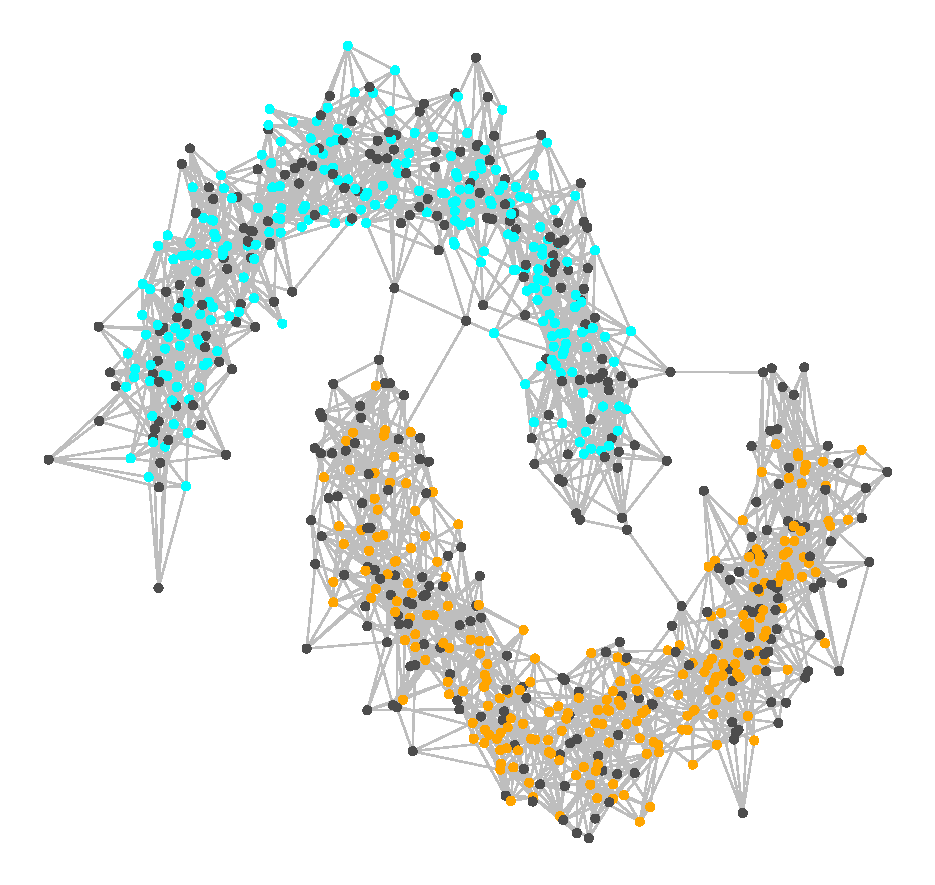
\includegraphics[width=\linewidth]{example2plots/row4_true_density_cluster}
			\caption{}
		\end{subfigure}
		\begin{subfigure}{.24\linewidth}
			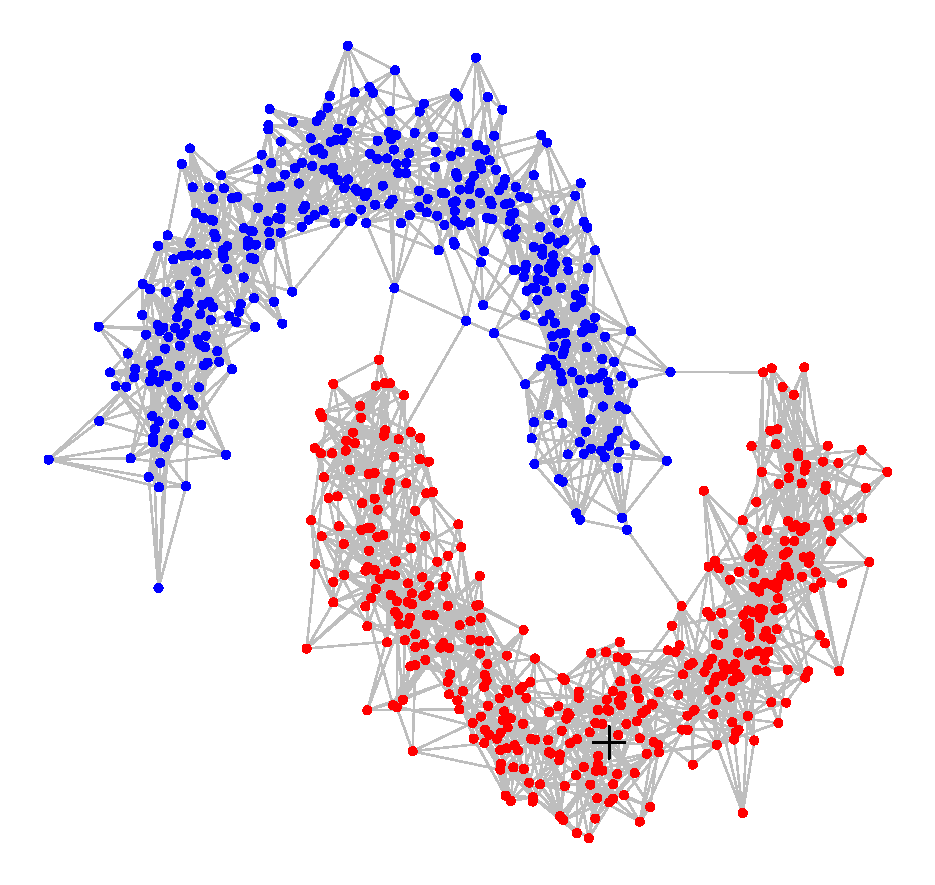
\includegraphics[width=\linewidth]{example2plots/row4_ppr_cluster}
			\caption{}
		\end{subfigure}
		\begin{subfigure}{.24\linewidth}
			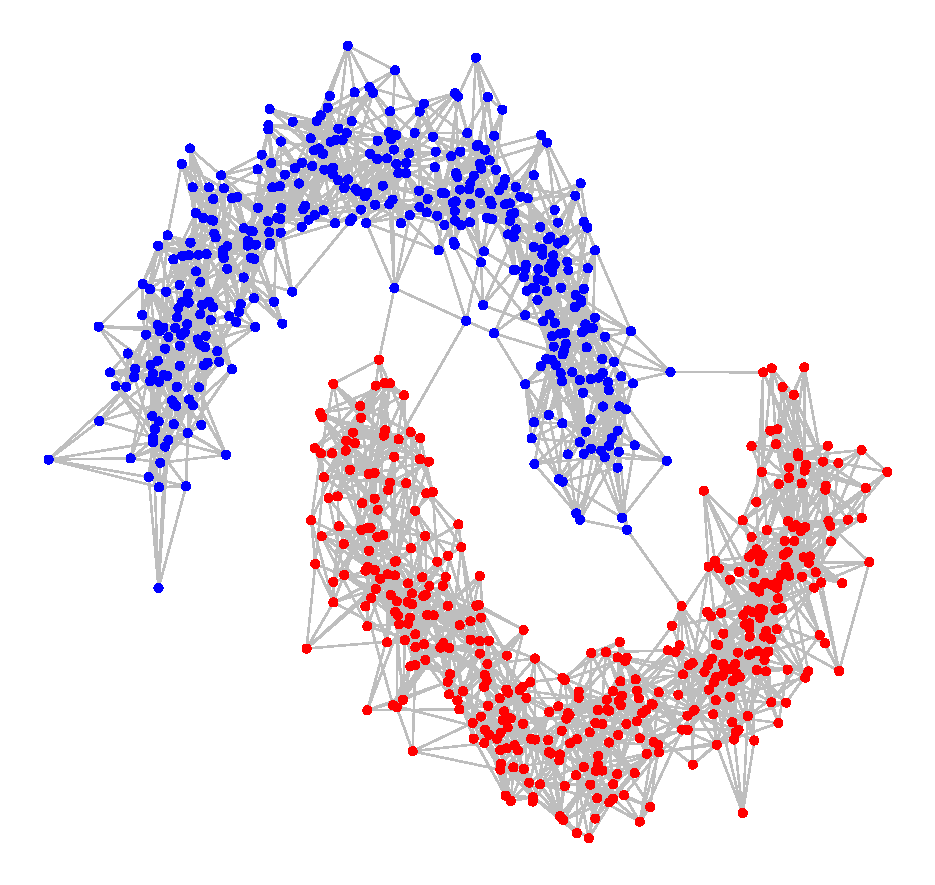
\includegraphics[width=\linewidth]{example2plots/row4_conductance_cluster}
			\caption{}
		\end{subfigure}
		\begin{subfigure}{.24\linewidth}
			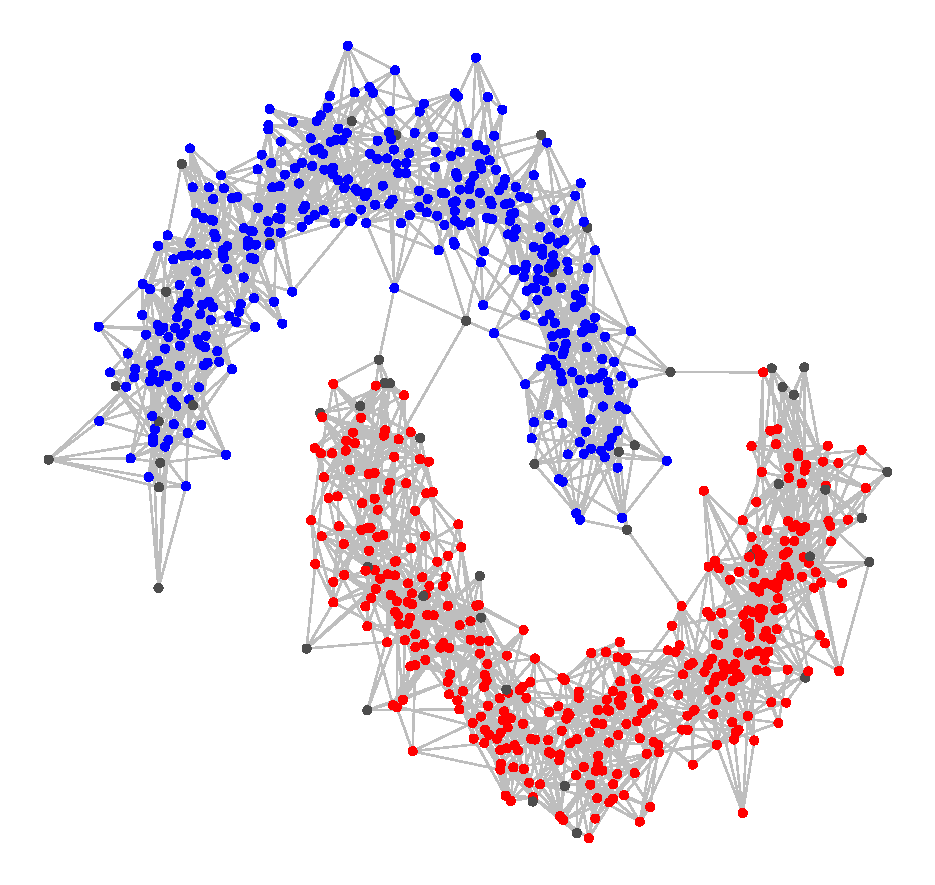
\includegraphics[width=\linewidth]{example2plots/row4_density_cluster}
			\caption{}
		\end{subfigure}
		\caption{}
		\label{fig:fig3}
	\end{adjustbox}
\end{figure}

\bibliographystyle{plainnat}
\bibliography{../local_spectral_bibliography}

\end{document}